
%\def\filepath{C:/Users/holden-lee/Dropbox/Math/templates}

\documentclass[12pt]{book}
\usepackage{etex}
%this prevents the "No room for a new \dimen" error that comes from loading too many packages (tikz+xy in particular)

%load geometry first (sets up page)
\usepackage[top=1.2in, bottom=1.2in, left=1in, right=1in]{geometry}

%main packages
\usepackage{amscd}
\usepackage{amsmath}
\usepackage{amssymb}
\usepackage{amsthm}
\usepackage{array}
\usepackage{bbm}
%\usepackage{asymptote}
\usepackage{cancel}
\usepackage{chemarrow}
\usepackage{cmap}
\usepackage{courier}
\usepackage[usenames,dvipsnames]{color}%%%
%\usepackage{color}
\usepackage{ctable}
\usepackage{enumerate}
\usepackage{enumitem}%resume lists
\usepackage{fancyhdr}
\usepackage{listings}
\lstset{
	basicstyle=\small\ttfamily,
	keywordstyle=\color{blue},
	language=python,
	xleftmargin=16pt,
}
\usepackage{makeidx}
%\usepackage{marvosym}%doesn't work
\usepackage{mathdots}%iddots: dots going northeast
\usepackage{mathtools}
\usepackage{mathrsfs}
%\usepackage{hyperref}
%\usepackage{sidecap}
\usepackage{stackrel}
\usepackage{stmaryrd}%\mapsfrom
\usepackage{tabularx}
\usepackage{tikz}
\usepackage{titlesec}
\usepackage{titletoc}
\usepackage{url}
\usepackage{verbatim}
\usepackage{wasysym}
\usepackage{wrapfig}
\usepackage{yhmath}
%\usepackage{yhmath}%arcs
\usepackage[all,cmtip]{xy}%Commutative diagrams
%\usepackage[usenames,dvipsnames]{xcolor}%tikz loads xcolor


\usepackage[usenames,dvipsnames]{color} % Required for specifying custom colors and referring to colors by name
\usepackage[pdftex]{hyperref} % For hyperlinks in the PDF
\hypersetup{
  colorlinks=true,
  linkcolor=MyBlue, 
  citecolor=MyRed,
  urlcolor= MyBlue
}

\definecolor{MyRed}{rgb}{0.99, 0.0, 0.0} 
\definecolor{MyGreen}{rgb}{0.0,0.4,0.0} 
\definecolor{MyBlue}{rgb}{0.0, 0.0, 0.6}

%load hyperref last
%\usepackage{hyperref}
%\usepackage{listings}
%\lstset{
%	basicstyle=\small\ttfamily,
%	keywordstyle=\color{blue},
%	language=python,
%	xleftmargin=16pt,
%}
%this causes an error. No idea why.

\usetikzlibrary{calc,trees,positioning,arrows,chains,shapes.geometric,%
    decorations.pathreplacing,decorations.pathmorphing,shapes,%
    matrix,shapes.symbols,shadows,fadings}

%\input xy
%\xyoption{all}

%http://www.simonsilk.com/content/simonsilk/2011-jun/latex-list-notations-nomenclature
\usepackage[refpage]{nomencl}
\renewcommand{\nomname}{List of Notations}
\renewcommand*{\pagedeclaration}[1]{\unskip\dotfill\hyperpage{#1}}
\makenomenclature
%The first line invokes the nomenclature package, and the option refpage means that the list will include, for each symbol in the list,  the page number on which you added it with the \nomenclature command. Leave it out to remove page numbers. The second line is the title at the top of the list of notations. The third line changes the page numbers in the list so they are right-justified with a line of dots connecting them back to the description of the symbol. By default, they follow the description after a comma and the word "page." The last line tells Latex you're using nomenclature so it will generate and look for the associated intermediate files during successive runs.

\makeindex

\setcounter{tocdepth}{3}
\setcounter{secnumdepth}{3}
%\pagenumbering{arabic}

%http://tex.stackexchange.com/questions/142982/how-to-get-the-current-chapter-name-section-name-subsection-name-etc?lq=1
\usepackage{etoolbox}
% Patch the sectioning commands to provide a hook to be used later
\preto{\chapter}{\def\leveltitle{\chaptertitle}}
\preto{\section}{\def\leveltitle{\sectiontitle}}
\preto{\subsection}{\def\leveltitle{\subsectiontitle}}
\preto{\subsubsection}{\def\leveltitle{\subsubsectiontitle}}

\makeatletter
% \@sect is called with normal sectioning commands
% Argument #8 to \@sect is the title
% Thus \section{Title} will do \gdef\sectiontitle{Title}
\pretocmd{\@sect}
  {\expandafter\gdef\leveltitle{#8}}
  {}{}
% \@ssect is called with *-sectioning commands
% Argument #5 to \@ssect is the title
\pretocmd{\@ssect}
  {\expandafter\gdef\leveltitle{#5}}
  {}{}
% \@chapter is called by \chapter (without *)
% Argument #2 to \@chapter is the title
\pretocmd{\@chapter}
  {\expandafter\gdef\leveltitle{#2}}
  {}{}
% \@schapter is called with \chapter*
% Argument #1 to \@schapter is the title
\pretocmd{\@schapter}
  {\expandafter\gdef\leveltitle{#1}}
  {}{}
\makeatother
%%%%%%%%%%%%%%%%%%%%%%%%%%%%%%%%%%%%%%%%%%%%%%%%%
%%%Theorem styles
\newtheoremstyle{norm}
{12pt}
{12pt}
{}
{}
{\bf}
{:}
{.5em}
{}

\newtheorem{thm}{Theorem}[section]
\newtheorem*{thm*}{Theorem}
\newtheorem{clm}[thm]{Claim}
\newtheorem*{clm*}{Claim}
\newtheorem{conj}[thm]{Conjecture}
\newtheorem*{conj*}{Conjecture}
%\newtheorem{cons}{Construction}
\newtheorem{cor}[thm]{Corollary}
\newtheorem{lem}[thm]{Lemma}
\newtheorem*{lem*}{Lemma}

\theoremstyle{norm}
\newtheorem{prb}[thm]{Problem}%[section]
\newtheorem*{prb*}{Problem}

\newtheorem{alg}[thm]{Algorithm}
\newtheorem{ax}[thm]{Axiom}
\newtheorem*{ax*}{Axiom}
\newtheorem{df}[thm]{Definition}
\newtheorem*{df*}{Definition}
\newtheorem{ex}[thm]{Example}
\newtheorem*{ex*}{Example}
\newtheorem{exr}[thm]{Exercise}
\newtheorem{expl}[thm]{Exploration}%prb
\newtheorem{fct}[thm]{Fact}
\newtheorem{mdl}[thm]{Model}
\newtheorem{pos}[thm]{Postulate}
\newtheorem*{pos*}{Postulate}
%\newtheorem{sprb}{Problem}%numbering for solutions
\newtheorem{pr}[thm]{Proposition}
\newtheorem*{pr*}{Proposition}
\newtheorem{qu}[thm]{Question}
\newtheorem*{qu*}{Question}
\newtheorem{rem}[thm]{Remark}
\newtheorem*{rem*}{Remark}

%%%%%%%%%%%%%%%%%%%%%%%%%%%%%%%%%%%%%%%%%%%%%%%%%

%%%%%%%%%%%%%%%%%%%%%%%%%%%%%%%%%%%%%%%%%%%%%%%%%
%%DEFINING BOX COMMANDS
\newcommand{\prbox}[1]{{
\noindent
\centering
\begin{tikzpicture}
\node [prbox] (box){
\begin{minipage}[l]{6in}
#1
\end{minipage}
};
\end{tikzpicture}\\%
}
}
\newcommand{\prbbox}[1]{\prbox{\begin{prob}#1\end{prob}}}
\newcommand{\expbox}[1]{\prbox{\begin{expl}#1\end{expl}}}
\newcommand{\sprbbox}[1]{\prbox{\begin{sprb}#1\end{sprb}}}

\newcommand{\thbox}[1]{{
\noindent
\centering
\begin{tikzpicture}
\node [thbox] (box){
\begin{minipage}[l]{6in}
#1
\end{minipage}
};
\end{tikzpicture}\\%
}}
%6.68

\newcommand{\thmbox}[1]{\thbox{\begin{theorem}#1\end{theorem}}}
\newcommand{\dfbox}[1]{\thbox{\begin{df*}#1\end{df*}}}

\newcommand{\grbox}[1]{{
\noindent
\centering
\begin{tikzpicture}
\node [cpbox] (box){
\begin{minipage}[l]{6in}
#1
\end{minipage}
};
\end{tikzpicture}\\%
}}
\newcommand{\cpbox}[1]{{
\noindent
\centering
\begin{tikzpicture}
\node [cpbox] (box){
\begin{minipage}[c]{.2in}
%\hspace{-.2in}
%\dbend
\includegraphics[scale=0.35]{\filepath/key}
\end{minipage}
\begin{minipage}[t]{6in}%6.25
#1
\end{minipage}
};
\end{tikzpicture}\\%
}}


\newcommand{\wrbox}[1]{{
\noindent
\centering
\begin{tikzpicture}
\node [wrbox] (box){
\begin{minipage}[c]{.2in}
%\hspace{-.2in}
%\dbend
{\Huge \bf !}
\end{minipage}
\begin{minipage}[t]{6in}%6.25
#1
\end{minipage}
};
\end{tikzpicture}\\%
}}
\newcommand{\hintbox}[1]{{
\noindent
\centering
\begin{tikzpicture}
\node [hnbox] (box){
\begin{minipage}[l]{6in}
\textbf{Hint:} {#1}
\end{minipage}
};
\end{tikzpicture}\\%
}
}
%white box
\newcommand{\whbox}[1]{{
\noindent
\centering
\begin{tikzpicture}
\node [hnbox] (box){
\begin{minipage}[l]{6in}
{#1}
\end{minipage}
};
\end{tikzpicture}\\%
}
}
%6.68
%END DEFINING BOX COMMANDS
%%%%%%%%%%%%%%%%%%%%%%%%%%%%%%%%%%%%%%%%%%%%%%%%%

%Box commands
%\thbox{...} makes a theorem box
%\thmbox{...} makes a theorem box labeled "Theorem"
%\prbox{...} makes a problem box
%\prbbox{...} makes a problem box labeled "Problem"
%\cpbox{...} makes a concept box labeled "Concept"
%\wrbox{...} makes a warning box.
%\dfbox{...} makes a definition box (same as problem box) labeled "> Definition"
%\sprbbox{...} makes a problem box labeled "Problem" (use this when you're making a copy of a previous problem box to put the solution afterwards; it has a numbering system separate from problems).

 
% for testing purposes only
\usepackage[english]{babel} 
\usepackage{blindtext} 
%%%%%%%%
%begin doc
%%%%%%%%
%%%%%%%%%%%%%%%%%%%%%%%%%%%%%%%%%%%%%%%%%%%%%%%%%
%DEFINING THE BOXES.
% Problem box (simple box, blue)
\tikzstyle{prbox} = [draw=black, fill=blue!20, very thick,
    rectangle, inner sep=10pt, inner ysep=10pt]
% Theorem box (double border, gray)
\tikzstyle{thbox} = [draw=black,double, fill=blue!10, very thick,
    rectangle, inner sep=10pt, inner ysep=10pt]
%\tikzstyle{fancytitle} =[fill=red, text=white]
% Concept box (shadowed, light green)
\tikzstyle{cpbox} = [drop shadow={
    shadow scale=1}, draw=black, fill=green!10, very thick,
    rectangle, inner sep=10pt, inner ysep=10pt]
\tikzstyle{wrbox} = [drop shadow={
    shadow scale=1}, draw=black, fill=yellow!10, very thick,
    rectangle, inner sep=10pt, inner ysep=10pt]
\tikzstyle{hnbox} = [draw=black, fill=white, very thick,
    rectangle, inner sep=10pt, inner ysep=10pt]
%END DEFINING BOXES
%%%%%%%%%%%%%%%%%%%%%%%%%%%%%%%%%%%%%%%%%%%%%%%%%


\renewcommand{\thesection}{\arabic{section}}
%% this file is for things that cannot go in the individual chapters, but only
%% in the main document

\newcommand{\rref}[1]{\cref{#1}}
\newcommand{\textnormal{}}[1]{\textnormal{#1}}

\renewcommand{\thethm}{\arabic{chapter}.\arabic{section}.\arabic{thm}}

\def\name{Mathematical Physics}


\pagestyle{fancy}
%\addtolength{\headwidth}{\marginparsep} %these change header-rule width
%\addtolength{\headwidth}{\marginparwidth}
\lhead{PHY521/MAT597}
\chead{} 
\rhead{Mathematical Physics} 
\lfoot{} 
\cfoot{\thepage} 
\rfoot{} % !! Remember to change the problem set number
\renewcommand{\headrulewidth}{.3pt} 
%\renewcommand{\footrulewidth}{.3pt}
\setlength\voffset{0in}
%\setlength\textheight{648pt}

\begin{document}
%\input{\filepath/titlepage.tex}
%\maketitle


\title{Mathematical Physics}
\author{Lectures by Professor Michael Aizenman \\ Scribes: Holden Lee and Kiran Vodrahalli}
% INCLUDE Scribes: Holden Lee & Kiran Vodrahalli
\maketitle

%\tableofcontents

\startcontents
\printcontents{ }{-1}{}

\chapter*{Introduction}
Notes from Michael Aizenman's class ``Mathematical Physics" at Princeton in Spring 2016. 

This class is of interest to both physicists and mathematicians. Several recent Fields medals are for work related to these topics.

%don't assume knowledge
I plan to cover the following topics. The focus is on \textbf{Topics in Mathematical Statistic Mechanics}.
\begin{enumerate}
\item
\textbf{The statistical mechanic perspective}: systems can be described at the microscopic level with many degrees of freedom. We observe their collective behavior and find emergent behavior.
\item
\textbf{Thermodynamics principles}:
%fasci
%macroscopic description of physical system 
Intellectually preceding statistical mechanics is thermodynamics, a field of physics which emerged through experimental and intellectual work trying to understand what is happening with the transfer of heat. A couple of principles emerged. This framework is more appropriate to the macroscopic description of physical systems.
In departure from mechanics, which cares about equalities like $F=ma, E=mc^2$, a unique thing about thermodynamics is that its key principle is in inequality: entropy increases.
\be
\Delta S\ge 0
\ee
%Entropy comes up as a emergent phenomenon from the statistical mechanics description of reality.
\item
\textbf{The emergence of thermodynamics from statistical mechanics via the equidistribution assumption and the ``large deviation theory"}. %vadhan - abel prize for large deviation theory.
I would like to discuss the emergence of thermodynamics from statistical mechanics. Mathematicians formalized the theory but the concepts were introduced earlier by physicists. These principles led Boltzmann to introduce these ideas and it took a while for physics to absorb the ideas.\footnote{This may have led to his premature death via suicide.}
\item 
\textbf{Phase transitions}: %Consider $H_2O$. You can control it by temperature and pressure. 
When you have a system, say $\text{H}_2\text{O}$, which you can control with temperature and pressure, you can induce changes in state. Continuous change in control parameters results in discrete jumps in the result. 

\item 
\textbf{Critical phenomena, critical exponents, universality classes}. Phase transitions are fascinating since there are interesting critical phenomena which are characterized by critical exponents, which turn out (this is one of the suprising discoveries experimentally) to result in universality classes of critical phenomena. Systems are macroscopically different, but the singularities you observe are given by the same power laws.
%Wilson.
\item
\textbf{Exact solution of the 2-D Ising model}. %From the perspective of physics. 
Mathematically, 3 is the hardest dimension to comprehend.
\begin{enumerate}
\item
1-D is solvable: correlations can be described by Markov chains, and can be computed. 
\item
In 2-D, the conformal group is very important. It gives many constraints on critical behavior, leading to a rich behavior. 
\item
In 3-D, this does not apply except for ongoing work finding consequences in 3-D from results in 2-D. 
\item
Anything with $\ge 4$ dimensions gets simpler. High dimensions are characterized by the fact that loop effects do not play a large role. In 1-D a simple random walk is recurrent. In sufficient high dimensions, a simple random walk is not recurrent.
The infinite-dimensional case reduces to models on trees; high dimensions exhibit the same behavior as infinite dimensions.
\end{enumerate}
In coding theory and discrete math people study phase transitions of different graphs and are interested in the same topics.

The 2D Ising model is usually a highly specialized topic, but we will do it in a way done a bit differently from normal. We would like to do this through ``graph zeta functions''. What I found fascinating about this topics is that there are a lot of connections to other topics. There are analogues of the Riemann zeta function on graphs, and there is a relationship. It is actually one of the simplest paths to tackle this proof by. 

\item
\textbf{Stochastic geometry behind correlation functions at criticality}: in the Ising model we have a collection of spin variables $\sigma_x=\pm1$ for $x\in \mathbb{Z}^d$. The spins are correlated in such a way that agreement among neighbors is encouraged. Thus there are correlations which spread through the system. 

It is interesting and powerful to represent this correlation between spins is via a ``shadow system'' in which you play the following game: decompose the collection of spins at random into connected clusters. You see spin values but you don't see who is connected to whom. %: But for each such decomposition the spins are connected on each cluster. 
An analogy is that students form cliques in class, and then each clique chooses what to do and votes unanimously. So if you just saw the voting pattern, you would see some cliques, but the nature of correlations among the votes become transparent if you know the clusters. 

The states for critical Ising models become larger, but also become fractal. Fractal geometric objects can be used to explain the structure. There is an interesting fractal geometry which tells us about correlation functions.

We will introduce all of this later in much detail from the ground up. This is related to percolation.

\item \textbf{Scaling limits}: Finally, if time permits, I would like to discuss scaling limits. You may want to know properties of a substance when you have something like a lattice that is very fine-grained, a statistic mechanical system which macroscopically is described by a myriad of variables. There are techniques of describing the relevant quantities from the macroscopic perspective, and this becomes relevant for describing the critical state. This provides a fascinating link between statistical mechanics and field theory. It's related to quantum field theory, except we are now in the Euclidean regime. There are some related results for quantum spin systems. 


\end{enumerate}
%random operators
%weekly packages

In a way we have a mouthful here, and one could probably give a full course on each of these topics. I will try not to be exhaustive, as we may not progress far. Previously I gave a course on random operators. Each week would cover some area of this subject, saying enough so you have a glimpse of the essence and get some comfort, and then moving on. It's now in a book format, and I would count it as a success if out of these lectures, something similar would emerge. The idea is not to be exhaustive, but to give enough key results. There is much more to be said, but I do not suppose to cover it all.

There is a broad spectrum of references, none of which I'll follow exclusively. 
\begin{itemize}
\item
Sacha Friedli and Yvan Velenik's online book project (on mathematical statistical mechanics) at \url{http://www.unige.ch/math/folks/velenik/smbook/index.html}. I recommend this for people totally new to the subject.
\item
David Ruelle formulated models and basic results mathematically (late 70's). His book helped physicists organize their thoughts. It became outdated quickly, but remains a good starting point and reference for the formalism.
\end{itemize}



%\setcounter{chapter}{-1}

\chapter{Introduction to statistical mechanics}

{\color{blue}2-2-16}

\section{Canonical Ensembles for the Lattice Gas}
\subsection{Configurations and ensembles}
One way to start is with the axioms of statistical mechanics. Instead I'll take a simple problem, see how it works, and present results in that context. There are simple problems that teach us a lot. (``The elementary problems are the most precious, once you absorb them they are part of your makeup.") The simplest is a lattice gas.

\begin{definition}[Lattice gas]
A \index{lattice gas}\textbf{lattice gas} is a substrate where at each lattice site there may or may not be a particle. This model has been used to describe alloys where you have a substrate which you can draw as a simple lattice (in particular, we will use $\mathbb{Z}^d$ for simplicity). Each point may have a particle of a certain type.

The \index{configuration}\textbf{configuration} is a function $n:\mathbb{Z}^d\to \{0,1\}$:
\be
n_x=\begin{cases}
1,&\text{$x$ is occupied},\\
0,&\text{$x$ is vacant}.
\end{cases}
\ee
For now let us ignore energy conservation. Let us suppose the system is neutral, or at some infinite temperature; energy is not an issue. 

I'll use $L$ to denote the size of the box we are considering, and $\Lambda\subset \mathbb{Z}^d$ to be a region (subset of the system) and we have $m$ particles. The \textbf{configuration space} is the space of possible $n$'s, $\Omega = \{0,1\}^{\Lambda}$.

If you have a finite system and energy does not play a role, but there is conservation of the number of particles, if you shake the box the state may change. Essentially each configuration gets equal weight, and particles do not overlap. 
\end{definition}


\begin{definition}[\index{Equidistribution assumption}\textbf{Equidistribution assumption}]
All particle configurations which have an equal number of particles have equal probability.
\end{definition}

This gives rise to the notion of ensembles. 
\begin{definition}[Ensemble]
An \textbf{ensemble} is a probability measure with respect to which you do averages over the configuration space $\Omega$. 
\end{definition} 
First, we define some notation.
\begin{definition}[Indicator function]
\be
\mathds{1}[\text{cond}] := \begin{cases}
1,&\text{condition satisfied}\\
0,&\text{else}
\end{cases}
\ee
\end{definition}
Now we define two specific ensembles, the \index{microcanonical ensemble}\textbf{microcanonical ensemble} and the \index{grand canonical ensemble}\textbf{grand canonical ensemble}. 

\begin{definition}[Microcanonical ensemble]
In the microcanonical ensemble,
\be
\mathbb{P}(n_{\Omega})= \frac{\mathds{1}[\sum_{x\in \Omega}n_x=N]}{Z}
\ee
where $Z$ is a normalization constant.

For every function $f:\Omega\to \mathbb{R}$ assigning a real number to each configuration, define the \index{microcanonical ensemble average}\textbf{microcanonical ensemble average} by
\be
\left\langle {f}\right\rangle_{N,n}^{\text{Can}} = \frac{\sum_{n\in \Omega} \mathds{1}[n_x=N] f(n)}{\sum_{n\in \Omega} \mathds{1}[\sum n_x=N]}.
\ee
\end{definition}
The ensemble we will focus on for this course is the grand canonical ensemble. 

\begin{definition}[Grand canonical ensemble]
The \index{grand canonical ensemble average}\textbf{grand canonical ensemble average} is defined as
\be
\left\langle {f}\right\rangle_{\mu, \Lambda}^{\text{Gr.C}} = \frac{\sum_{n\in \Omega} e^{-\mu  \sum_{x\in \Lambda}n_x}f(n)}{\sum_{n\in \Omega}e^{-\mu \sum_{x\in \Lambda} n_x}}
\ee
(Later on we will omit superscripts where it is clear.)
\end{definition}

We can relate these two notions with the \index{equivalence principle}\textbf{equivalence principle}. 

\begin{definition}[Equivalence principle]
Loosely, the equivalence principle says that for any ``local function", the microcanonical average is approximately the grand canonical ensemble average
\be
\left\langle {f}\right\rangle_{N,\Lambda}^{\text{Can}}\approx \left\langle {f}\right\rangle_{\mu, \Lambda}^{\text{Gr.C}}
\ee 
when we take $\mu = \frac{N}{|\Lambda|}$.
%at suitable $\mu=\mu\pf{N}{n}$.
\end{definition}


\subsection{The equivalence principle}

Consider functions which depend only on a system $\Lambda\subset \widetilde{\Lambda}$ of much smaller volume, $|\Lambda|\ll |\widetilde{\Lambda}|$. This is the sense in which the averages match up.

%sociological interest. 
We can think of the difference as the difference between two socities. One is draconian. The first is highly centralized control economy. If you don't fit the build, you get weight $0$ and you're thrown out. In the grand canonical, everything goes. Some contribute more than others, and the contributions depend on the parameter $\mu$ which is adjustable. The density of particles depends on $\mu$. And there is a value of $\mu$ for which the density is equal to $N/|\tilde{\Lambda}|$. Here, the average of the draconian system is equal to the average of the lackadaiscal system, asymptotically. 

The micro-canonical ensemble is draconian: the number of particles is prescribed, all other configurations get weight 0. %if don't fit bill get weight 0. 
In the grand canonical ensemble, each configuration contributes. There is a value of $\mu$ where the density is the same; at that value the local average of the draconian system is asymptotically the same at that of the more relaxed system. This $\approx$ becomes $=$ when you take the thermodynamic limit,
\begin{align*}
\widetilde{\Lambda} & \to \mathbb{Z}^d\\
N & \to \infty\\
\frac{N}{|\widetilde{\Lambda}|} & \to \rho.
\end{align*}

%If all that matters it the number of particles in $\La$, then we care about the induced distribution on $\La$. %What is the probability distribution 
Now let us see where this comes from. What is the induced distribution of the micro-canonical ensemble on $\Lambda$? If all you care about is the number of particles in the average you care about, you just care about getting a small system. If the whole system has a large number of particles, then it does not matter if you focus on a much smaller box since you can trade particles very easily, if the larger volume has a ton of particles. Under the microcanonical ensemble, the probability that $n_{|\Lambda}$ ($n$ restricted to $\Lambda$) takes a particular value depends only on one quantity, which is the number of particles the configuration has ($\sum_{\Lambda} n_x = k$ in the big box). This expression is equal to the cardinality (number) of configurations in the rest of the big box ($n_{|\Lambda^c}$, $\Lambda$ complement) such that the total number of points in $\Lambda^c$ is equal to $N - k$. And that of course must be normalized. Now we come to the question of how many configurations there are in the complement of $\Lambda$.

%n_{\Ga_n}
 %If you specify a configuration in $\L$
We count the number of ways to complete the configuration in $\Lambda^c=\widetilde{\Lambda}\backslash \Lambda$:
\begin{align*}
\frac{|\left\{{n_{\Lambda^c}}:{\sum_{x\in \Lambda^c}n_x=N-k}\right\}|}{Z}
\end{align*}
where $Z$ is a normalization constant.

The number of configurations of $M$ particles in volume $V$ is $\binom{V}{M} = \frac{V!}{M!(V-M)!}$. Using Stirling's approximation
\be
\ln (M!) = M(\ln M-1)(1+o(1)),
\ee
%gymnastics of elementary type.
%Boltzmann grade in Vienna
%entropy
After some gymnastics of an elementary nature, there is a fundamental formula. The logarithm of the number of configurations is of tremendous important. Ludwig Boltzmann's grave has the formula which opened people's eyes to what this mysterious \index{entropy}\textbf{entropy} $S$ truly is: the logarithm of the number of configurations. 

\begin{lemma}[Entropy]
Defining
\be
s(\rho) = -[\rho \ln \rho + (1-\rho)\ln (1-\rho)],
\ee
we have
\be
\binom{V}{M} = \frac{V!}{M!(V-M)!} 
=: e^{S(M,V)}
\approx e^{Vs(\rho)}
\ee
where density $\rho = m/V$ and $s(p) = -p\ln(p) - (1- p)\ln(1 - p)$. 

The ratio $\rho$ varies between $0$ and $1$. $s(\rho)$ is concave and attains maximum of $\ln 2$ at $\frac{1}{2}$ where it has quadratic behavior.
\end{lemma}
\begin{proof}
Please do this exercise once in your life; it's good to do it once but not too often.
\end{proof}
Shannon also found such a formula for entropy.

The implication is that if you slightly change the density, the number of configurations changes drastically. In physical substances $V$ may be $10^{23}$. The change would then be $e^{10^{23}\Delta s}$. In any average over configurations, only those at the peak contribute: ``winner takes all."

What is the probability of observing $k$ particles in the small box given $n$ in the big box?
\begin{align*}
\mathbb{P}(n_{\Lambda}) &\approx \frac{e^{|\Lambda^c|s\left( {\frac{N-k}{|\widetilde{\Lambda}| - |\Lambda|}} \right)}}{Z} %\quad \rh=\fc{N}{|\wt{\La}|}
\end{align*}
where $Z$ is a normalizing constant. The probability is propotional in exponent to the volume of the complement multiplied times the entropy of the density, which we saw in the exercise above. Then we re-write the density of the small box in terms of the overall density: 
\begin{align*}
\frac{N-k}{|\widetilde{\Lambda}|-|\Lambda|}&=\rho - \underbrace{\left( {\rho - \frac{N}{|\widetilde{\Lambda} | - |\Lambda|}} \right)}_{\to 0 \text{ independent of $k$}} -
\frac{k}{|\widetilde{\Lambda}|-|\Lambda|}
\end{align*}
The entropy is infinitely differentiable except at the endpoints, so we can just expand. Whatever you see inside affects the number outside, but does not effect the density outside. This explains why we only have a tiny correction to $\rho$. Thus 
\begin{align*}
s\left( {\frac{N-k}{|\widetilde{\Lambda}|-|\Lambda|}} \right) & \approx s(\rho) - s'(\rho)\frac{k}{|\Lambda^c|}
%particles here is small fraction of number of outside.
\end{align*}
Changing $k$ by a little bit affects how many particles are outside but not so much the density outside: the correction term is small. Hence for $\sum_{x\in \Lambda}n_x$,
\be
\mathbb{P}(n_\Lambda) \approx \frac{e^{|\Lambda^c|s(\rho)}e^{-s'(\rho)k}}{Z}.
\ee
$e^{|\Lambda^c|s(\rho)}$ is a huge factor but it does not vary with $k$ so we can omit it. Writing out $Z$ as the sum of the numerators over all $n_\Lambda$,  and letting $\mu = s'(\rho)$, we get that this equals
\be
=\frac{e^{-\mu k}}{\sum_{n'\in \Omega_{\Lambda}}e^{-\mu\sum_{x\in \Lambda} n'_x}},
\ee
which is the grand canonical ensemble average.
So all you have to do is be sure to pick $\mu$ as the derivative of the thermodynamic function at the correct density. That is how we derive the canonical ensemble in this case. 
The rest of the system acts on the small system as a ``particle (heat) bath."
%\begin{theorem}[Equivalence principle]
%Let $f:\Om \to \R$ be a function depending 
%\end{theorem}

Here we used very explicit machinery, namely, the Stirling formula. We want a general expression that doesn't rely on the Stirling formula because in more complicated models, we will not have the luxury of using the Stirling approximation. We'll do this in the next section.

%Note we can also apply this method 
Then we will be able to consider models where there are more energy constraints. The general procedure is first make a list of energy constraint. There is a generalization of the equivalence principle where 
\begin{itemize}
\item
in the micro-canonical ensemble we average over configurations where the constraints have prescribed values. (We considered the special case where just the number of particles was prescribed.) %meet the constraint. All of them get equal weight.
\item 
in the grand canonical ensemble, we add an energy term to the exponential: $e^{-\mu N(n) - \beta\mathcal{E}(n)}$ where $N(n)$ is the number of particles, $-\mu N(n)$ is the Gibbs factor, and $\mathcal{E}(n)$ the energy.
\end{itemize}
%Functions which depend on a small region, can be computed with Gibbs factors, $e^{-\mu N(n) - \be\cal E(n)}$ where $N(n)$ is the number of particles, $-\mu N(n)$ is the Gibbs factor, and $\cal E(n)$ the energy.

How can we construct an alternative method without the Stirling formula?



{\color{blue}2-4-16}

%Lattice gas
%$\La, M$ particles
%$n:\La\to \{0,1\}$
%Configuration space $\Om=\bit^{\La}$.
%Study particles within region. The fact that the total number of particles is fixed is less visible in a small region.
%For the grand canonical ensemble, we have independence.
%Can: $\Pj(n) = \fc{\one[N(n)=M]}{C}$, 
%The grand canonical ensemble $\fc{e^{-\mu N(n)}}{Z_\La(\mu)}$.
%we can compute using the entropy.
%how without stirling.
\subsection{Generalizing Ensemble Analysis to Harder Cases}

Previously we used very specific machinery to derive the grand canonical ensemble for the lattice gas; how might we derive similar expressions for more complicated systems?  We would like to avoid using the Stirling formula, which only happened to work in the simple case. 
To derive the entropy bypassing Stirling's approximation, you may proceed by analyzing partition functions. 

Define the \index{partition function}\textbf{partition function} for the grand canonical ensemble as the (unnormalized) sum of the likelihoods over all configurations. At each site there are 2 possibilities and they are independent, so the sum factors into a product.\footnote{Note that $\Lambda$ in the last section is the micro-canonical ensemble, but here it is the grand canonical ensemble.}
\begin{align}
\nonumber
Z_\Lambda & = \sum_{n\in \Omega} e^{-\mu N(n)} \\
\nonumber
&=\sum_{n\in \Omega} \prod_{x\in \Lambda} e^{-\mu \mathds{1}[n_x=1]}\\
\nonumber
&=\prod_{x\in \widetilde{\Lambda}}(1+e^{-\mu})\\
\nonumber
&= (1+e^{-\mu})^{|\Lambda|}\\
\frac{1}{|\Lambda|} \ln Z_{\Lambda} &= 1+e^{-\mu}
\label{eq:z1}\text{{\color{red}\tiny eq:z1}}
\end{align}

So what does this have to do with entropy? We can calculate $Z_\Lambda$ a different way, as follows.
Note that the only thing that matters in the summand is the number of particles in $n$, so let's group the summands by this. Letting $\rho=\frac{N}{|\Lambda|}$, and using the fact that the number of states with density $\rho$ is $e^{|\Lambda|s(\rho)}$,\footnote{Rather than getting this with $s(\rho)=-[\rho\ln(\rho) - (1-\rho) \ln (1-\rho)]$ by the Stirling approximation in the last section, we can take this as the \emph{definition} of $s$ here, and use it to solve for $s$.}
\begin{align}
\nonumber
Z_\Lambda&=\sum_{n\in \Omega} e^{-\mu N(n)}\\
\nonumber
& \approx \sum_{\rho \in \frac{1}{|\Lambda|}\mathbb{Z}} e^{-\mu N(n)} e^{|\Lambda|s(\rho)}\\
\nonumber
& =\sum_{\rho \in \frac{1}{|\Lambda|}\mathbb{Z}} e^{|\Lambda|[s(\rho)-\mu \rho]}\\
%concave modified by a linear function.
%for each $\mu$ there is some maximum.
%when you look at contribution of points $\ep$ away, it changes by a factor of the volume. 2
%all terms which are $\ep$ away contribute a negligible amount.
\label{eq:z2}\text{{\color{red}\tiny eq:z2}}
&\approx e^{|\Lambda|\max_{\rho\in [0,1]}[s(\rho)-\mu\rho]}.
\end{align}
%The multiplicity is the exponential of the volume $|\La|$ times the entropy $s(\rh)$.
%Should we should multiply by the range . 
To get the last step, note that the error we are making by focusing on the maximal point rather than counting with multiplicity the near-maximal value is at most a factor equal to the volume, since we can upper bound our error by taking all points in $\Lambda$ instead of merely an $\varepsilon$-ball around the maximum. ``In analysis, it often pays to avoid being excessively generous.'' Since $\frac{1}{|\Lambda|}\ln |\Lambda|\to 0$, this term is negligible. %details to follow
%excessively meticulous.
The expression $\max_{\rho\in [0,1]}[s(\rho)-\mu\rho]$ is called the \index{Legendre transform}\textbf{Legendre transform} of the entropy and denoted by $s^*(\rho)$. 

Matching~\eqref{eq:z1} and~\eqref{eq:z2}, we find
\be
s^*(\mu):= \max_{0\le \rho\le 1} [s(\rho) - \mu\rho] = \ln (1+e^{-\mu})
\ee
%this isn't a definition.
%can define 
%\begin{definition} Legendre entropy. \\
%\beq{eq:s-leg}
%s^*(\mu):= \max_{0\le \rh\le 1} [s(\rh) - \mu\rh] = \ln (1+e^{-\mu})
%\eeq
%\end{definition}

%The maximal value of $\fc KV$ takes it all: this is

Using this, we can derive the expression the formula for $s(\rho)$, using the inverse Legendre transform.

To check that taking the maximum in~\eqref{eq:z2} was legit, note that\footnote{Mathematicians are paranoid, so we use $\sup$ instead of $\max$. For many practical purposes they are the same.}
\begin{align*}%\llabel
\max_{\rho}[s(\rho) - \mu \rho] &\le \frac{1}{|\Lambda|}\ln Z_{\Lambda} \le \max_\rho [s(\rho)-\mu \rho] + \underbrace{\frac{1}{|\Lambda|}\ln |\Lambda|}_{\to 0}\\
\implies
\lim_{|\Lambda|\to \infty} \frac{1}{|\Lambda|}\ln Z_{\Lambda} &= \sup_{0\le \rho\le 1} [s(\rho) - \rho \mu].
\end{align*}
%We know this is true because 
%from the partition function we can extract the entropy.
%consistent with Stirling formula? Can we do without? Yes.

%comment: This is essentially the same as the series of equations~\eqref{eq:s2}.
%Now why is this equation true? It's a very fundamental point. This is true since we applied Stirling to the counting function, which comes from the fact that when you compute the partition function, it's the sum over all allowed configurations: $Z_N = \sum_{m \in \Omega} e^{-\mu N(m)}$. Let's classify these terms according to the value of $N$. Recall density $\rho$ is just number of particles per volume: $N/ |\Lambda|$. Let's write $N(m) = \rho\cdot |\Lambda|$. Thus we can rewrite $Z_N = \sum_{\rho_{1/|\Lambda|}} e^{-\mu \rho |\Lambda|}e^{|\Lambda|s(\rho)} = \sum_{\rho_{1/|\Lambda|}} e^{|\Lambda|(s(\rho) - \mu \rho)}$. $\rho \in [0, 1]$ and we discretize over $1/|\Lambda|$. As we saw before, we use the maximum because when we deviate a small amount from the maximum, a \textbf{slight drop}, all terms which are $\epsilon$ away, contribute an entirely negligible amount. 
%Hence 
%\be
%\max_{0\le \rh\le 1}[s(\rh) - \mu\rh] = 1+e^{-\mu}
%\ee
%This is essentially Legendre transform. It is in particular invertible.
%Stirling's approximation gave us the answer for the entropy. Any other model: you will not have the luxury of the Stirling approx argument. 

We can verify that  $s(\rho) = -[\rho\ln \rho +(1-\rho) \ln (1-\rho)]$
does indeed make~\eqref{eq:s-leg} hold. We find the maximum (critical point) or $s(\rho)-\mu \rho$ by setting the derivative to 0.\footnote{Don't differentiate in public.} 
We use the trick 
\be[x(\ln x-1)]'=\ln x.\ee We can subtract 1 from each of the logs changing the expression by a constant. Thus
\be
s'(\rho) = -\ln \rho +\ln (1-\rho) - \mu \implies \frac{\rho}{1-\rho}=e^{-\mu}.
\ee
We can use this to solve for $\rho$ and find $s^*(\mu)$ (do this yourself).
%Solving gives $\fc{\rh}{1-\rh}=e^{-\mu}$. 

In general, a micro-canonical ensemble specifies all the conserved quantities: Particles, energies, and whatever else there is. The grand canonical ensemble also generalizes by changing the factor to $e^{-\mu N} e^{\beta H}$.
Such factors are referred to as \index{Gibbs factors}\textbf{Gibbs factors} %states
or Gibbs measures.
%variational characterization of those.
%Our next topics are:
%\begin{itemize}
%\item
%Legendre transform
%\item
%Convexity/concavity
%\item A variational characterization of Gibbs states
%\item First order phase transitions (thermodynamics and statistical mechanics perspectives)
%\end{itemize}

\section{Concavity and the Legendre transform}

\subsection{Basic concavity results}

\begin{definition}
A function on $\mathbb{R}^k$ is \index{concave}\textbf{concave} if for any $x_0,x_1\in \mathbb{R}^k$, $0\le \lambda \le 1$,
\be
F(\lambda x_1+(1-\lambda)x_0)\geq \lambda F(x_1)+(1-\lambda) F(x_0).
\ee
For a \index{convex}\textbf{convex} function, the same inequality with the sign flipped holds. A negative convex function is concave. 
Concavity (convexity) means if you draw a chord between two points, it will lie below (above) the curve.\footnote{``As Richard Feynmann pointed out, getting the sign right is the hardest thing.''}
\end{definition}
%A concave curve frowns.

%useful for variational principle
For a strictly concave function, a maximum, whenever it exists, is unique.
%Feynman: getting the sign right is the hardest thing.

\begin{theorem}
For any concave function on $\mathbb{R}$, 
\begin{enumerate}
\item
The directional derivatives $F'(x\pm0)$ exist at all $x\in \mathbb{R}$. The \index{directional derivative}\textbf{directional derivative} is defined as
\begin{align*}
F'(x+0)&=\lim_{\varepsilon\to 0^+} \frac{F(x+\varepsilon)-F(x)}{\varepsilon}\\
F'(x-0)&=\lim_{\varepsilon\to 0^-} \frac{F(x+\varepsilon)-F(x)}{\varepsilon}.
\end{align*}
\item $F'(x-0)\ge F'(x+0)$ and $F'(x\pm 0)$ are decreasing.
\item For all but countably many values $x\in \mathbb{R}$, $F'(x-0)=F'(x+0)$, i.e., $F$ is differentiable at $x$.
\item Let $F_n$ be a sequence of concave functions which converge pointwise: for all $x$, $\lim_{N\to \infty} F_N(x)=:\widetilde{F}(x)$ exists. 
Then
\begin{enumerate}
\item
 $\widetilde{F}$ is concave.
\item
At points of differentiability of $\widetilde{F}$, the derivatives also converge,\footnote{Finite energy functions are always smooth, but %as a baby's face
their limit can have discontinuous derivative.
%Converge pointwise without derivative converging.
}
\be
F'(x\pm 0) \to \widetilde{F}'(x).
\ee
\end{enumerate}
\end{enumerate}
\end{theorem}

\begin{center}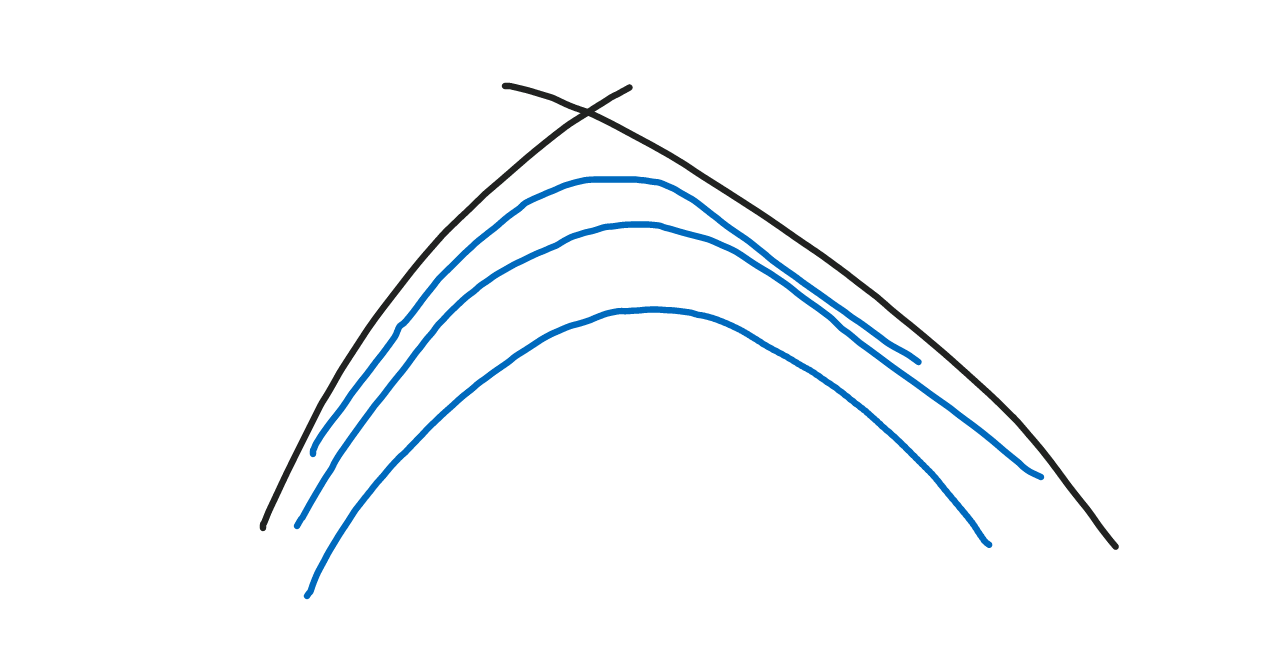
\includegraphics[scale=.25]{images/2-3}\end{center}

Much of this generalizes to directional derivatives in $n$ dimensions.
\begin{proof}
For (1) note that concavity implies that the slope of the line between $x,x+\varepsilon$ is increasing as $\varepsilon\to 0^+$.

\begin{center}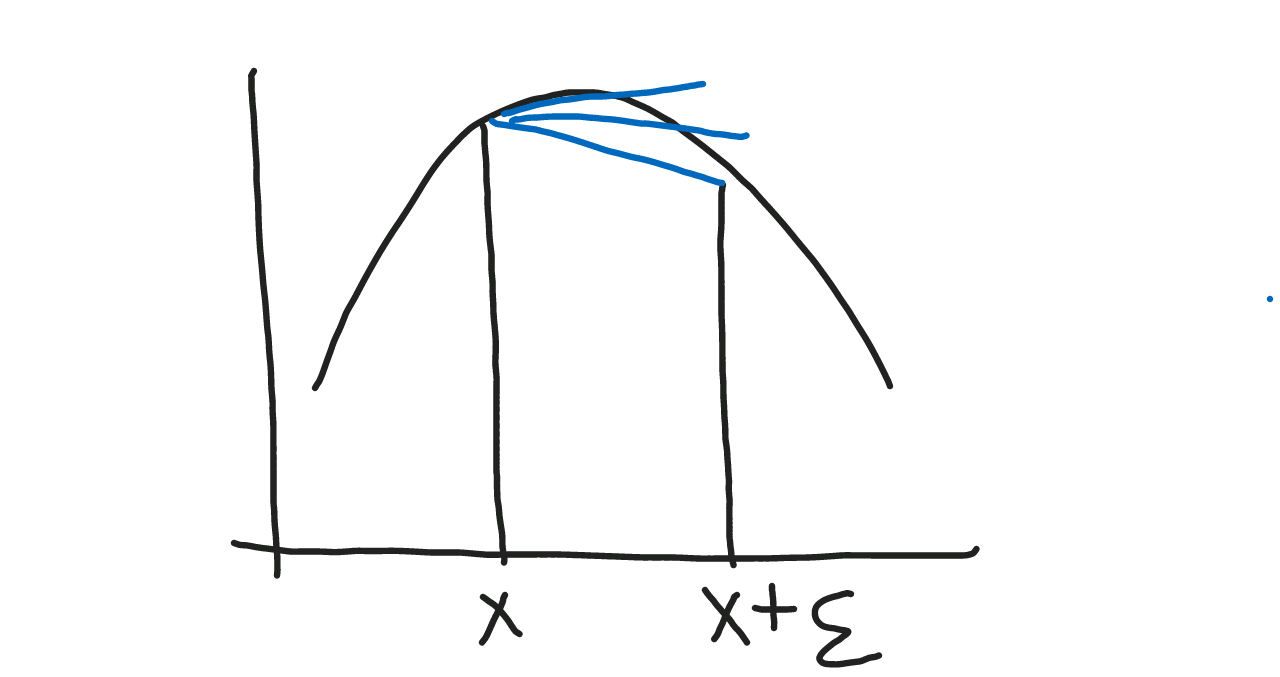
\includegraphics[scale=.25]{images/2-1}\end{center}

%The slope of the line between $x,x-\ep$ is decreasing as $\ep\to 0^-$.
To prove (3), consider the graph of the derivative $F'(x + 0)$. It's a monotone decreasing function: it starts somewhere and goes down. 
%Rewrite
At points where $F'(x+0)$ is continuous, we have $F'(x+0)=F'(x-0)$. The discontinuities, or ``steps," are the points where $F'(x+0)\ne F'(x-0)$. Now we use the fact that the sum of any uncountable collection of nonzero numbers is $\infty$. 
Applying this to the steps, we find that the number of steps is countable, i.e., the total collection of discontinuity points has to be countable.\footnote{More rigorously, for every nonzero interval $[F'(x+0),F'(x-0)]$, we can associate with it a rational number. Then note $\mathbb{Q}$ is countable.}
%Hence, if you have a function which decreases by steps, the total collection of discontinuity points has to be countable.
%It may actually decrease by steps. A nice thing about monotone steps is that a sum of any uncountable collection of nonzero numbers is $\infty$.\footnote{More rigorously, for every nonzero interval $[F'(x+0),F'(x-0)]$, we can associate with it a rational number. Then note $\Q$ is countable. } If you have a function which decreases by steps, the total collection of discontinuity points has to be countable. %The total sum of the drops is finite, which implies that the number of drops is actually finite. 
%This is FALSE: it can be countable.
%At points where there is a continuity, they agree. They only disagree at points of discontinuity. Since we have summable jumps, the collection of points of discontinuity is at most countable.
\footnote{The set of discontinuities can still be devilishly dense, ex. all the rational numbers. In physics it used to be thought that weird functions with Cantor-like sets of discontinuties could not occur, but there are materials whose free energy discontinuities are dense in certain areas.}

\begin{center}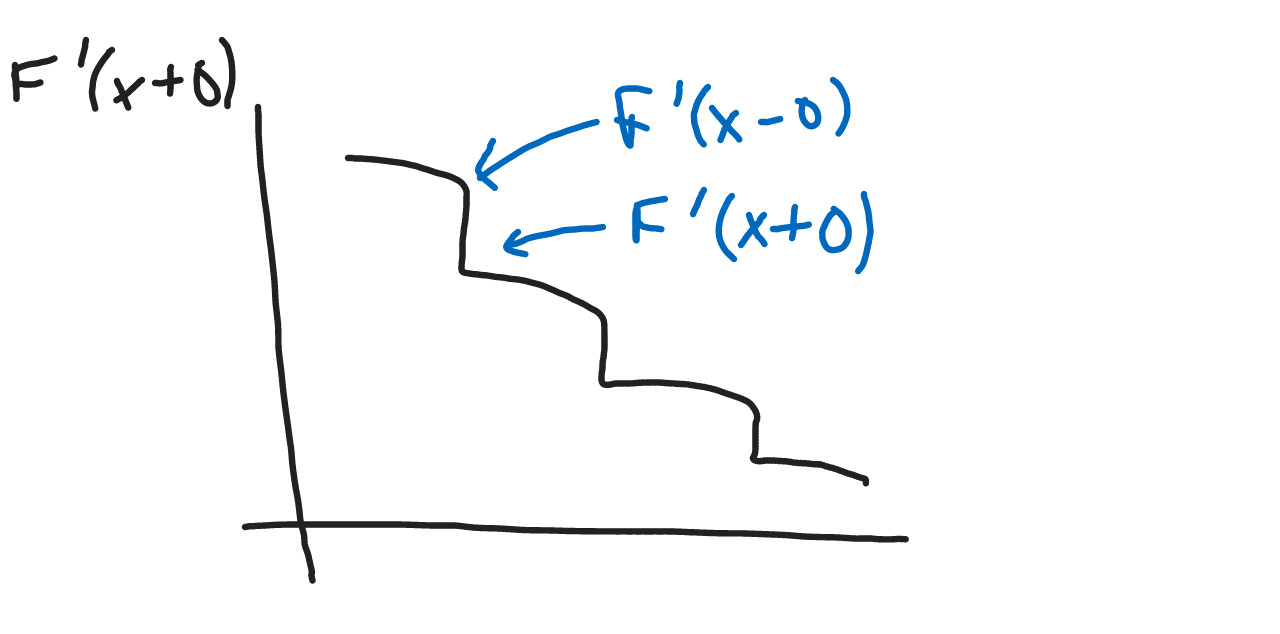
\includegraphics[scale=.25]{images/2-2}\end{center}
\end{proof}

\subsection{Concave properties of the Legendre transform}

\begin{definition}
The \index{Legendre transform}\textbf{Legendre transform} of a function is defined as
\be
(TG)(y) = \inf_x [y\cdot x - G(x)] = - \sup_x [G(x) - y\cdot x]
\ee
\end{definition}
\begin{theorem}
For any function $G$, $TG$ is concave.
\end{theorem}
%You can futz with $\ep$, but from a certain angle this is immediate.
\begin{proof}
An efficient way to think about this is the following: for each value of the parameter $x$, as a function of $y$ this is a linear function. For each $x$ we get a linear function. Define the transform by taking the infimum over that. 

Take 2 points and draw the chord between them. For each linear function the chord lies below it.\footnote{I.e., we use the following : Let $\mathcal{F}$ be a collection of concave (e.g. linear) functions. Then $\inf_{f\in \mathcal{F}}f(x)$ is concave.} 

\begin{center}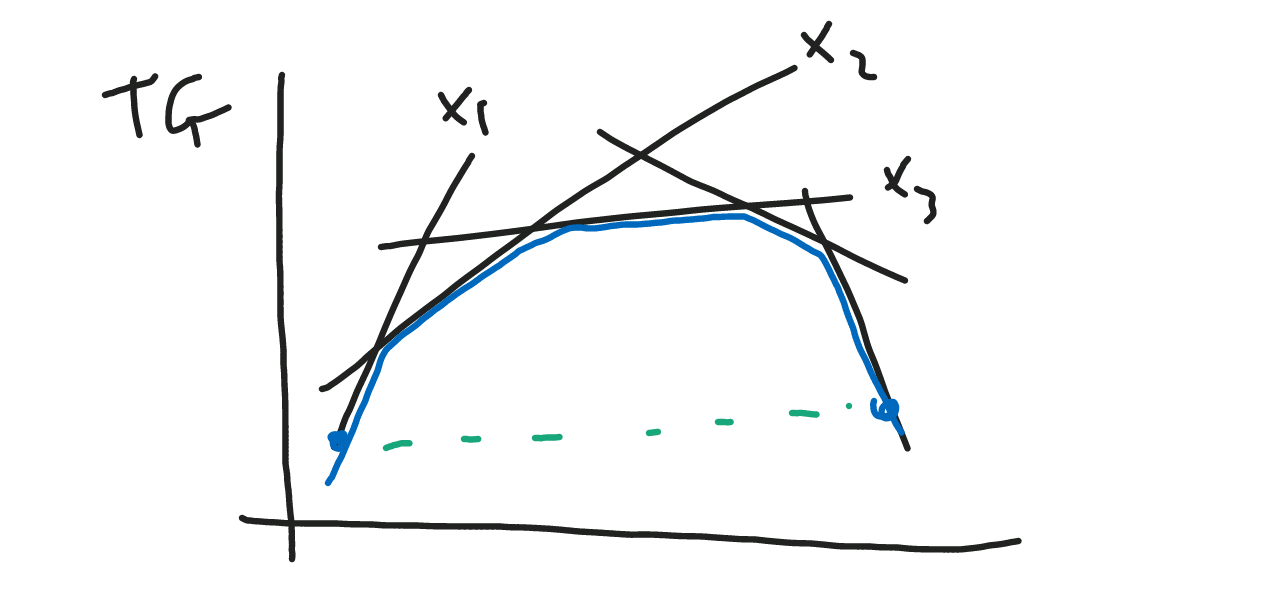
\includegraphics[scale=.25]{images/2-4}\end{center}
\end{proof}
\begin{definition}
The \index{concave hull}\textbf{concave hull} $\widetilde{G}$ of $G$ is defined as the smallest concave function that is at least the function value at every point:
\be
\widetilde{G}(x)=\inf \left\{{F(x)}:{F\text{ concave, }\forall u, \,F(u)\ge G(u)}\right\}.
\ee
%look at all functions that are concave and dominate it.
\end{definition}

\begin{center}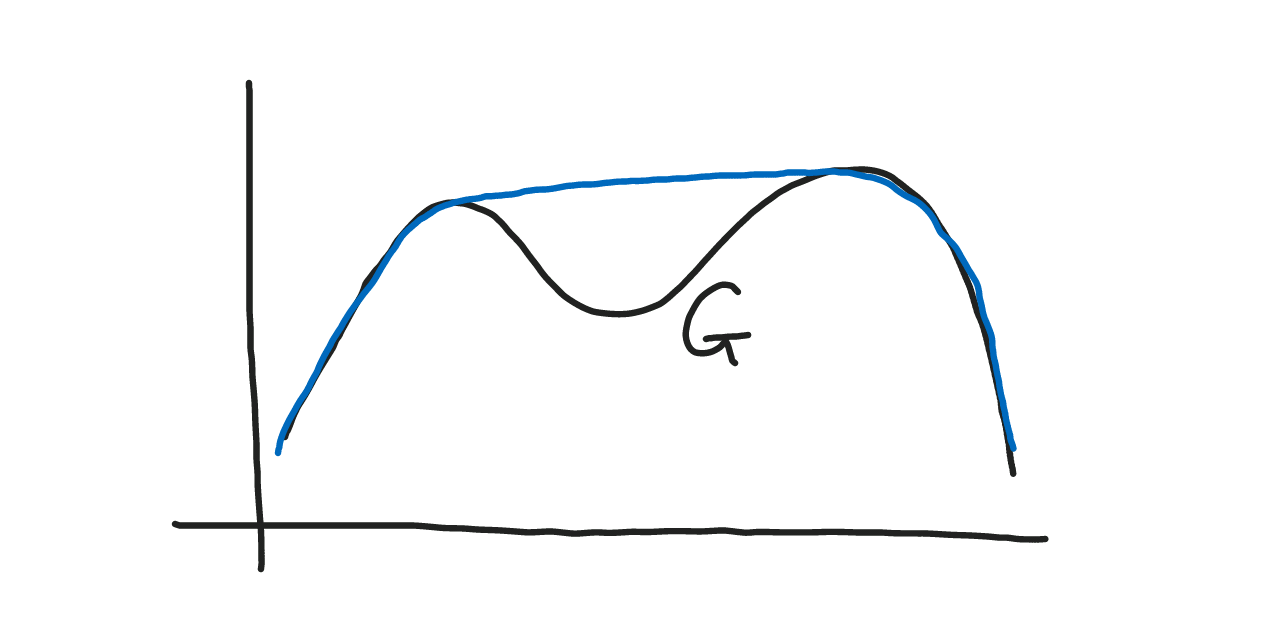
\includegraphics[scale=.25]{images/2-5}\end{center}

\begin{theorem}
For \emph{concave} $G$,
\be
T(TG)=G.
\ee
In general, $T(TG)$ is the concave hull of $G$. 
\end{theorem}
\begin{proof}[Proof for $G$ differentiable]
Use the fact that if $G$ is differentiable, then
\be
\inf_x [y\cdot x - G(x)]
\ee
occurs at $y=G'(x)$. %learn about function in discontinuous fashion. exactly what happens in 1st order phase transitions.
\end{proof}

Note that we plotted the function and the dual function on the same graph. However, they have inverse units, for example, energy and inverse temperature. You get a lot of insights into physics if you keep track of the units.
%energy and inverse temperature. You get a lot of insights into physics if you keep track of the units. Note $x,y$ have inverse units.


Recall $\rho=\frac{N}{|\Lambda|}$. %prob within configurations of observing something.
If all $2^{|\Lambda|}$ configurations are given equal weight, the typical value or $\rho$, the particles per unit volume is $\frac{1}{2}$. The Law of Large Numbers says that with probability 1 the ratio tends to $\frac{1}{2}$. Is it possible that the density is $\frac{1}{3}$? Yes, but the probability of such a density is given by the entropy: it's exponentially small, $e^{|\Lambda|[s\left( {\frac{1}{3}} \right) -\ln 2]}$. Anything other than $\frac{1}{2}$ is a large deviation; they occur with exponentially small probability. We want to quantify the probability of large deviation events. Here is a language that people found useful.
\begin{definition}\label{df:ldp}\text{{\color{red}\tiny df:ldp}}
A sequence of probability measures on $\mathbb{R}$ is said to satisfy a \index{large deviation principle}\textbf{large deviation principle} with speed $\{a_N\}$, and rate function $I(x)$ if for each $x\in \mathbb{R}$, $\varepsilon>0$,
%raghu vadhan
\be
-\inf_{|u-x|<\varepsilon} I(u)\le 
\varliminf_{N\to \infty}\frac{1}{a_N} \ln \mathbb{P}_N((x-\varepsilon,x+\varepsilon]) \le \varlimsup_{N\to \infty} \frac{1}{a_N} \ln \mathbb{P}_N((x-\varepsilon,x+\varepsilon]) \le 
-\inf_{|x-u|\le \varepsilon} I(u)
\ee
%much more complicated situations
\end{definition}
For us, $I(x)=\ln 2 - s(x)$.
%This definition generalizes the situation where the previous applies.



{\color{blue}2-9-16: Today we'll talk about Gibbs states: definition, variational principle, and relations to thermodynamic foundations.}

\begin{theorem}[Jensen's inequality]
\index{Jensen's inequality}
Let $\rho(dx)$ be a probability measure on $\mathbb{R}$ ($\mathbb{R}^d$) with finite expectation $\int |X| \rho(dx)<\infty$, and let $F:\mathbb{R}\to \mathbb{R}$ be a concave function. Then
\be
\int F(X)\rho(dx) \le F\left( {\int X\rho(dx)} \right).
\ee
\end{theorem}
To remember this, draw a picture. Consider the case where the measure is concentrated on two points. The interpolated value $\int F$ is less than the function value $F(\int)$. (In the case of two points, this is the definition of Jensen.)

\begin{center}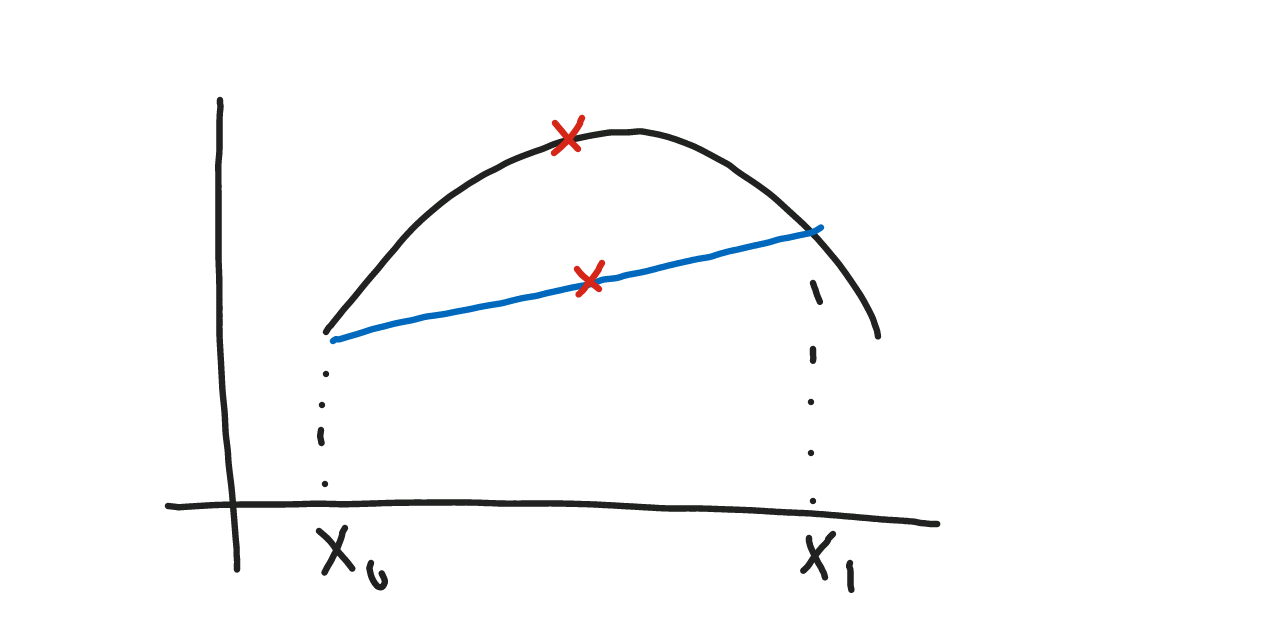
\includegraphics[scale=.25]{images/3-1}\end{center}

\begin{proof}
Let $\left\langle {X}\right\rangle = \int X\rho(dx)$. Take any tangent to $F$ at $\left\langle {X}\right\rangle$. 
Note that $F$ may not be differentiable, so take the line to have slope $F'(\left\langle {X}\right\rangle+0)$.
%Note that $F$ may not be differentiable, so by this we mean take a line passing through $(\an{X},F(\an{X}))$ with slope
%\be
%F'(\an{X}+0) \le \mu \le F'(\an{X}-0).
%\ee
%Then for all $x$, $F(x)$
The first inequality~\eqref{eq:jensen1} follows from concavity.
\begin{center}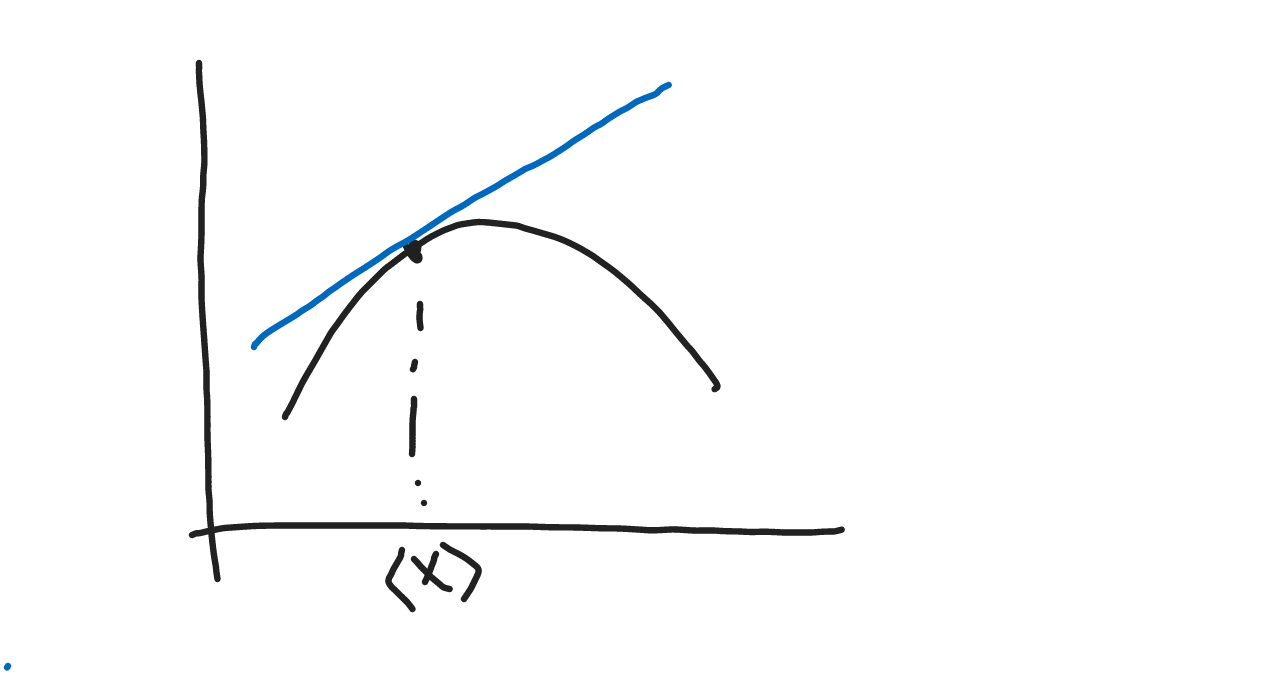
\includegraphics[scale=.25]{images/3-2}\end{center}
Integrate and note that $F(\left\langle {X}\right\rangle)$ is constant to get~\eqref{eq:jensen2}.
\begin{align}
\label{eq:jensen1}\text{{\color{red}\tiny eq:jensen1}}
F(X) &\le F(\left\langle {X}\right\rangle) + (X-\left\langle {X}\right\rangle) F'(\left\langle {X}\right\rangle+0)\\
\label{eq:jensen2}\text{{\color{red}\tiny eq:jensen2}}
\int F(X)\rho(dx)& \le \underbrace{F(\left\langle {X}\right\rangle)}_{\int \rho(dx)=1} + \underbrace{0}_{\int [X-\left\langle {X}\right\rangle]\,\rho(dx)=0}.
\end{align}
\end{proof}
This theorem is elementary but very useful. 

\section{Basic setup for statistical mechanics}
%The basic setup for statistical mechanics is as follows. 

The basic setup consists of... 

\begin{enumerate}
\item
A \textbf{lattice or a homogeneous graph} like $\mathbb{Z}^d$. %Often I'll use this as an example.
It will be important that for $\Lambda_L=[-L,L]^d$, 
\begin{equation}\label{eq:bdary-ratio}\text{{\color{red}\tiny eq:bdary-ratio}}
\frac{|\partial \Lambda_L|}{|\Lambda_L|} \xrightarrow{L\to \infty} 0.
\end{equation}

Here $|\cdot|$ means the size in terms of number of points (it doesn't matter much how you count---e.g. whether you count just the points on the edge, or adjacent too, etc.). \eqref{eq:bdary-ration} says when you chop space into regions, the boundary plays a small role. This is good becase we should be talking about extensive quantities.
\item
\textbf{Collection of local variables} like $\{n_x\}$ taking values in 0, 1, or $\{\sigma_x\}$ taking values in $\pm1$, magnetizations, etc.
%magnetization, other value of interest
\item
An extensive \index{energy function}\textbf{energy function}, defined on finite subsets. 
%interesting things happen in the infinite limit.
%Associate energy with finite subsets. 
For example, 
\be
H_{\Lambda}(\sigma)=-\sum_{(x,y)\subset \Lambda, |x-y|\le r}%\int_{x-y} 
\sigma_x\sigma_y - h\sum_{x\in \Lambda} \sigma_x.
%HL: not sure about this.
\ee
This is over a finite range; we can also consider unbounded ranges with some decay.

Here there are only pairwise interactions, but more generally, there can be interactions between more variables: 3, 4... Typically the interactions are translation invariant. The general equation is
\be
H_{\Lambda}(\sigma) = \sum_{A\subset \mathbb{Z}^d, \operatorname{diam}(A)\le R} K_A(\sigma),
\ee
where $K_A(\sigma)$ depends on $\sigma_{\upharpoonright A}$ ($\sigma$ restricted to $A$), and are shift covariant.

%finite range.
\item
%reference probability distribution.
A \textbf{reference a-priori (probability) measure} $\rho_0(d\sigma)$ (a probability distribution with respect to which we integrate) on the configuration space $\Omega_\Lambda$ ($=\{-1,+1\}^{\mathbb{Z}^d}$).

For example, $\rho_0(d\sigma)$ could be the product measure where $\{\sigma_x\}$ are iid variables. (Think of a system at high temperature.)\footnote{Note that it makes sense to talk about e.g. an infinite number of coin flips. There is such a thing as an infinite product of probability measures. In an infinite product space, the result of any finite collection is independent.  Any single value has probability 0.}\footnote{How does the Declaration of Independence go? ``We hold these truths to be self-evident... inalienable rights..." The definition of person is time-dependent. But there is a reference measure, individuals are treated equally. That's how we start in statistical mechanics. E.g. Every spin configuration gives equal value. If the spins are continuous, what would be a good starting point? Perhaps they are independently distributed on the sphere.}

We will also allow measures which are not probability measures---normalization may be ``part of the game."

Particle configurations are given by specifying locations and momenta. We can chop space into boxes, and specify the number of particles in each box, and their positions and momenta. The starting point is the Liouville measure, which is invariant under time evolution by the Hamiltonian.
\end{enumerate}

\subsection{Gibbs equilibrium measure}
\begin{definition}\label{df:gibbs-eq}\text{{\color{red}\tiny df:gibbs-eq}}
The finite-volume \index{Gibbs equilibrium measure}\textbf{Gibbs equilibrium measure} at temperature $T=\beta^{-1}$ is 
\begin{equation}\label{eq:gibbs-eq}\text{{\color{red}\tiny eq:gibbs-eq}}
\text{Prob}(d\sigma) = \frac{e^{-\beta H_{\Lambda}(\sigma)}}{Z_\Lambda} \rho_0(d\sigma_{\Lambda}).
\end{equation}
Here $Z_{\Lambda}$ is the normalizing (partition) function
\begin{equation}\label{eq:zla}\text{{\color{red}\tiny eq:zla}}
Z_{\Lambda}(\beta) = \int e^{-\beta H_\Lambda(\sigma_\Lambda)} \rho_0(d\sigma_A).
\end{equation}
\end{definition}
This is a \index{generating function}\textbf{generating function} because taking the derivatives we can learn about the distribution of the random variable.

The Gibbs equilibrium measure is the uniform measure %by tilting it with 
multiplied by the Gibbs factor. Here, $\beta$ is a factor corresponding to the inverse of the \index{temperature}\textbf{temperature}.

\begin{itemize}
\item
When $\beta=0$, local variables are independently distributed. We have chaos; all states are equally likely.
\item
When $\beta$ cranked up, i.e., temperature is lowered, the probability distribution becomes more concentrated (near the ``ground state"). When $\beta=\infty$, the distribution becomes concentrated on configurations which minimize the energy.
\end{itemize}•
We will see that the Gibbs equilibrium measure is the distribution of a system at thermal equilibrium at temperature $T$. Why is that so and what is the relation to microcanonical ensemble?

We will try to understand the structure of these measures and the phase transition they manifest.

\subsection{Introduction to the Ising model}

In biology, they study Drosophila, the fruit fly. Studying this simple organism tells us a lot.
The Ising model is the Drosophila of statistical physics. What you learn from it extrapolates to many other systems, but not everything.

%At low configurations, the configurations settle close to the ground state. 

Consider the \index{Ising model}\textbf{Ising model} on $\mathbb{Z}^d$,
\be
H_\Lambda(\sigma) = -\frac{1}{2}\sum_{|x-y|=1} J \sigma_x\sigma_y - h\sum_{x\in \Lambda} \sigma_x, \qquad J\ge 0.
\ee
At $T=0,\beta=\infty$, the state with all $+$'s and the state with all $-$'s are equally likely.
There is no continuous way to go from all spins $+$ to all spins $-$.
%analytic in finite volume may have nonanalytic limits.
%Nontrivial statement that the Gibbs function is analytic in $x$ for $h$ nonzero. Another statement, one of the general things you learn in statistical mechanics, is that for $H=0$ this is an analytic function even after you take the infinite limit. 
For nonzero, analytic even after take infinite limit.


However, the analyticity would fail, and in fact you would find a line of first order transitions at $H=0$ up to some temperature $T_c$. 
What happens is a natural extension at zero temperature and infinite $\beta$. You go from configuration that is all $+$ to all $-$ going through a discontinuity. 
The Gibbs state---the trivial distribution at this temperature---comes in 2 flavors (at least, other possibilities can hold): The state would remember whether the magnetic field $H$ was turned to 0 from the positive or negative side. This is a beautiful example of what you observe in magnets. 

The floor under the Atlantic ocean has ferromagnetic rocks. It was detected that the direction of magnetization changes. When you cool a ferromagnet (ferromagnets develops magnetic moments), which way it points is affected by the prevalent external field. According to prevailing wisdom, as the sea floor was expanding, the Earth's magnetic moment flipped. The rocks have encoded in them the direction of magnetization when they were cooled past this critical temperature. This phenomenon is called residual magnetization.
%There is a phenomenon of residual magnetization which remembers how it got to this state.. 
This phenomenon is eliminated when you raise to high enough temperature; then the state becomes the analytic. 
%infinite volume measure. 
We will discuss more about this phase transition, including behavior near the critical point, later.

This refers to the infinite volume limit of such measures. In finite volume, everything is analytic. 
At 0 temperature the configuration is all $+$, but at small temperature, thermal fluctuations occur. Unlike when $\beta=\infty$, when $\beta$ is finite, every local configuration gets some nonzero weight. Even thoguht there is a preference for agreement, the system exhibits fluctuations. Among the $+$'s there will be islands of minority spins. As temperature increase, minority fluctutions increase to a point where each spin tries to agree both with its neighbors and with magnetic field. When there is a lot of fluctuation among its neighbors, the effect of magnetic field is not so significant. That's how this discontinuity evaporates when you increase temperature.

\subsection{Entropy, energy, and free energy}
\begin{definition}
Let $\rho_0$ be a reference measure.
\begin{enumerate}
\item
For any probability measure $\mu$ on $\Omega_{\Lambda}$\footnote{that is absolutely continuous with respect to $\rho_0$}, we can write it in terms of $\rho_0$,
\be
\mu(d\sigma_\Lambda) = g(\sigma) \rho_0(d\sigma_\Lambda).
%ratio of the measures
\ee
The function $g(\sigma)$, the ``ratio" of the measures, is called the \index{Radon-Nikodym derivative}\textbf{Radon-Nikodym derivative}, and denoted by
\be
g(\sigma) = \frac{\delta\mu}{\delta\rho_0}.
\ee
%trace of density times log of density.
%canonical symbol is Radon-Nikodym derivative.
\item
Define the \textbf{entropy} of $\mu$ as
\be
S_\Lambda(\mu|\rho_0) = -\int g(\sigma_\Lambda)\ln g(\sigma_\Lambda) \rho_0(d\sigma_\Lambda).
\ee
\item Define the \index{energy content}\textbf{energy content} of $\mu$ as 
\be
E(\mu) = \int H_{\Lambda}(\sigma_{\Lambda}) \underbrace{g(\sigma_{\Lambda})\rho_0 (d\sigma_\Lambda)}_{\mu(d\sigma_A)}.
\ee

\end{enumerate}•
\end{definition}
%expected value of energy with respect to measure, entropy
\begin{theorem}\label{thm:gibbs-eq}\text{{\color{red}\tiny thm:gibbs-eq}}
For each $\beta\in [0,\infty)$, the Gibbs equilibrium measure~\eqref{eq:gibbs-eq} is the unique minimizer of 
\be
\beta F_\Lambda(\mu) := \beta E_{\Lambda}(\mu) - S_\Lambda(\mu|\rho_0),
\ee
equivalently, the unique maximizer of $S_{\Lambda}(\mu|\rho_0) - \beta E_{\Lambda}(\mu)$.
%negative temperature?
\end{theorem}
\begin{definition}
The quantity $\beta F_{\Lambda}(\mu)$ is called the \textbf{free energy}.
\end{definition}
We'll keep $\beta$ positive, but we can make sense of some of the theory when $\beta$ is negative. Sometimes we can even talk about $\beta$ complex!
%temperature is positive, otherwise call a doctor.

The second law of thermodynamics says that nature ``maximizes entropy under constraints." %Except at the thermal size, 
Here we're maximizing entropy minus energy. How to reconcile this? 
%it's constrainted in the microcanonical ensemble, not constrained in the grand canonical ensemble. 
There is some reservoir where the system trades with the entropy. As it trades off energy with the reservoir, the energy of the reservoir is affected. It is the effect of the entropy of the reservoir that the system has energy $E$. What the system is really maximizing is the entropy of the \emph{system and reservoir}.
%nice to think in terms of entropy

The free energy $\beta F_{\Lambda}(\mu)$ is the energy you get from the system when in thermal contact.\footnote{It's funny to talk about the energy crisis: we never run out of energy. The problem is that we have too little \emph{free} energy, we have too much entropy.}

%\begin{proof}[Proof of Theorem~\ref{thm:gibbs-eq}]
%Let $\rh_\be (d\si) = e^{-\be  H_\La(\si)}{Z_\La(\Ga)} \rh_0(d\si)$. Let $\psi(x)=-x\ln x$  which looks like the following.
%\ig{images/3-3}{.1}
%We bound the entropy using Jensen's inequality with $X= \fc{\de\mu}{\de \rh_\be}$,
%\bal
%S(\mu|\rh_0)&=-\int \fc{\de\mu}{\de\rh_\be} \ln \pf{\de\mu}{\de\rh_\be} \,\rh_\be (d\si_\La)\\
%& =\int \psi\pa{\fc{\de\mu}{\de\rh_\be}(\si_\La)}\rh_\be(d\si_\La)\\
%& \le \psi\pa{\an{\fc{\de\mu}{\de\rh_\be}}}=\psi(1)=0
%\end{align*}
%%average of concave function is below function at the midpoint
%%using $\an{X} = \int \fc{\de\mu}{\de \rh_\be}$, $\int \mu(d\si_\La)=1$, with 
%Equality holds if and only if 
%\be
%\fc{\de\mu}{\de\rh_\be} = \an{\fc{\de\mu}{\de\rh_\be} }= 1
%%evaluate what this means you end up with this expression.
%\ee
%where 
%\be
%\fc{\de\mu}{\de\rh_\be} = \fc{\de \mu}{\de \rh_0} \fc{Z_\La(\be)}{e^{-\be H_\la(\be)}}
%\stackrel{\text{claim}}= S(\La)(\mu|\rh_0)-\be E_{\La}(\mu).
%\ee
%%take the log
%To see the claim, note that the LHS is
%\bal
%&=\int \fc{\de\mu}{\de\rh_\be} \ln \pf{\de\mu}{\de\rh_0} \rh_\be(d\si)
%+ \ln Z_\La(\be) \ub{\int \fc{\de\mu}{\de\rh_\be}\rh_\be(d\si)}{=1} - \be \ub{\int \fc{\de\mu}{\de\rh_\be}H_{\La}(\si) \rh_\be (d\si)}{H_\La(\si) \mu(d\si_\La)}
%%energy function, last \de/\de. same as 
%%changes of notation, need experience.
%\end{align*}
%\fixme{This isn't quite right. I will post a complete derivation later. Change of variables?}
%\end{proof}
%By Jensen's inequality, the entropy is maximized when $S_{\La}(\mu|\rh_c)$. %, so it's uniquely maximized when equal to thermal state. 

What is the consequence? The thermal states are the states which maximize the difference. This allows to quantify the difference. When $\beta$ is small, the energy plays a minor role. The states maximize the entropy. As the temperature descreases and $\beta$ increases, $\beta E_\Lambda(\mu)$ in the variational principle plays an increasing role; the energy has to be low; $\beta$ controls how low it has to be. 

What's coming next? We'll pay attention to the factor $\ln Z_\Lambda(\beta)$. (Recall $Z_\Lambda(\beta)$ was defined in~\eqref{eq:zla}.) We will calculate 
\be\lim_{\Lambda \nearrow\mathbb{Z}^d} \frac{1}{|\Lambda_L|} \ln Z_{\Lambda}(\beta).\ee
%This ($S-\be E$) would be
%\be
%Z_{\La}(\be) = \int e^{-\be H_\La(\si)} \rh_0(\de).
%\ee
The relevant contribution comes only from configurations which are at an energy where the entropy is maximized. 

Entropy appears in many guises. We talked about entropy over a measure, but you can also talk about the entropy function of energy; the contribution from those particles would be $e^{S(E)}e^{-\beta E}$. Now it's just a function of the energy. This function picks up the Legendre transform of the entropy.
%It picks up the Legendre transform... as a function of energy. 

 %the contribution comes is $e^{-\

In the Ising model, there is a discontinuity in the nature of the states. Differentiability of the free energy function breaks down across the line. There is an interplay between convexity properties of thermodynamic functions. The left and right derivative---the mean values of the magnetization---corresponds to 2 different limiting values, that are the two different magnetizations depending on which way you arrive. %Concave functions of parameters.

Statistical mechanics translates into the nonuniqueness of Gibbs equilibriums state. Statistical mechanics provides much more information because it looks at the joint distribution of all these variables, whereas thermodynamics just fixes attention on a few relevant parameters. We will clarify this relation. 
We will clarify this and then discuss techniques to find the phase transitions.
%\section{A variational characterization of Gibbs States} 

%\section{First order phase transitions}



{\color{blue}2-11-16: I started a couple of lines of discussion involving entropy; I would like to tie up a few of those loose ends. Just to remind you, please do not hesitate to ask questions about notation and the like; we have a very mixed audience and it's good to be reminded of elementary questions.}

\begin{remark}
%Just a word about the configuration space for a finite system, perhaps 
Let $\Omega_0$ be the possible states (e.g., $\{-1, +1\}$ for spin states) for a single particle, and $\Omega = \Omega_0^G$ where $G$ is the lattice graph. Any $\sigma \in \Omega$ is in the form $\sigma = \{\sigma_x\}_{x \in G}$, where $\sigma_x \in \Omega_0$. 
%are something like the spin states ($\pm 1$). 
In the discrete case ($\Omega_0$ and $G$ are finite), the probability of configuration $\sigma$ is $\rho(\sigma) = \rho(\{\sigma\})$.
%For probability measures, with the discrete case it's given by $p(\{\sigma\})$. We might denote expectation for a finite space as 
The expectation in the discrete case is a sum,
\be
\mathbb{E}_{\rho}(f) = \sum_{\sigma \in \Omega} f(\sigma) \rho(\sigma).
\ee
%More generally, we would write this as an integral
In general, the expectation is an integral,
\be
\int f(\sigma) \rho(d\sigma).
\ee

Note that the sum is just integration respect to a discrete measure. The integral notation is more flexible because it adapts to non-discrete cases, for instance, when $\Omega_0 = S$ takes values on the sphere. 
\end{remark}


We talked about relative entropy, and entropy entered the situation different times in different ways. Entropy appears in many different areas, and they are all either related by precise relations or analogy. 

\begin{definition} 
%For a pair of probability measures $\rho, \mu$ with
Let $\rho,\mu$ be probability measures such that $\mu$ is absolutely continuous with respect to $\rho$. Let $\mu = G(\sigma)d\sigma$, i.e., $G=\frac{\delta\mu}{\delta\rho}$ is the Radon-Nikodym derivative with respect to $\rho$. 
The \textbf{relative entropy} is 
\be
S(\mu | \rho) = -\int G(\sigma) \ln(G(\sigma))\rho(d\sigma) = - \int \ln G(\sigma) \mu(d\sigma)
\ee
%Think of the cause where $\mu(d\sigma)$ is \vocab{absolutely continuous} with respect to $\rho$. This is denoted as the \vocab{Radon-Nikodym derivative} with respect to $\rho$ ($\frac{\delta\mu}{\delta\rho})$. 
\end{definition}

Before we talk about the Gibbs measure and the variational principle, let us give a useful lemma.

\begin{lemma} For any pair of probability measures, %(on a finite set, though this holds more generally) 
\be
S(\mu | \rho) \leq 0
\ee
with equality iff $\mu = \rho$ (as measures).
\end{lemma}
%We give this proof in essence, using Jensen's inequality.
%seems to just follow from concavity of $x\ln x$...
\begin{proof}
Take $\psi(x) = -x\ln(x)$. Look at the tangent line $(1 - x)$ intersecting the $x$-axis (see photo) and see that the function is less: 
\begin{align}
%\begin{split}
-x \ln(x) &\leq 1 - x
\label{eq:2-11-1}
\\
\nonumber
S(\mu | \rho) &= 
\int  \psi\left( {\frac{\delta\mu}{\delta\rho}} \right) \rho(d\sigma)\\
\nonumber
&=\int \left[ \psi\left( {\frac{\delta\mu}{\delta\rho}} \right) - \left( {1 - \frac{\delta\mu}{\delta\rho}} \right)\right]\rho(d\sigma)\\
\nonumber &\leq 0
%\end{split}
\end{align}
where we used the fact that the derivative of $\rho$ against the Radon-Nikodym derivative with respect to $\rho$ is just $1$, \be\int \left(\frac{\delta \mu}{\delta \rho} \right) \rho (d\sigma )= \int \mu (d\sigma) = 1,\ee 
so that $1-\frac{\delta\mu}{\delta\rho}$ integrates to $0$. We added this term order to use~\eqref{eq:2-11-1}. 
%Note that the 
\end{proof}
Hence, this is a variational principle for entropy. 

\begin{remark}
For cases where things are not absolutely continuous, we define the relative entropy to be $-\infty$, since things will blow up. 
\end{remark}

Now, we derive a useful relation for  $\rho_{\beta}(d\sigma)  = \frac{e^{-\beta H(\sigma)}}{Z} \rho_0 (d\sigma)$:
\begin{equation}\label{eq:2-11-2}\text{{\color{red}\tiny eq:2-11-2}}
S(\mu | \rho_0) - \beta \int H(\sigma) \mu d(\sigma) = \ln(Z) + S(\mu | \rho_{\beta})
\end{equation}
With a bit of political license, you may refer to this as the amount of free energy: It's $\beta$ times the entropy. %We mean energy in that particular state. 
%FIXME
\begin{proof}
%The LHS $- \ln(Z) =$
We have
\be
\left( {S(\mu | \rho_0) - \beta \int H(\sigma) \mu d(\sigma)} \right) - \ln (Z)=
-\int \ln\left(\frac{\delta\mu}{\delta\rho}\cdot \frac{Z}{e^{-\beta H(s)}}\right) \mu (d\sigma )
\ee
Now we must show this is the same thing as $S(\mu | \rho_{\beta})$. We can look at it slighlty differently, as though we are modifying the Radon-Nikodym derivative with respect to the modified measure. The above equals
\be
= -\int \ln\left(\frac{\delta\mu}{\delta\rho_{\beta}}\right) \mu d\sigma = S(\mu|\rho_{\beta})
\ee
by definition. 
\end{proof}
This is rather cool: It says a thermodynamic flavored quantity is equal to the relative entropy with respect to the Gibbs-measure plus a positive constant. %Equality holds only when we take entropy with respect to the Gibbs state. %FIXME

So with this we have proof of what we said last time.

\begin{thm*}[Theorem~\ref{thm:gibbs-eq}]
The (finite volume) \textbf{Gibbs equilibrium} measure $\rho_{\beta}(d\sigma)$ is the unique maximum of 
\be
-\beta F(\mu) := S(\mu|\rho_0) - \beta \int H(\sigma) \mu (d\sigma)
\ee
\end{thm*}
\begin{proof}[Proof of Theorem~\ref{thm:gibbs-eq}]
By \eqref{eq:2-11-2}, this equals $\ln Z + S(\mu|\rho_\beta)$. $S(\mu|\rho_\beta)$ is maximized for $\mu=\rho_\beta$.
\end{proof}

The point was to show that this measure would be dominated by the Gibbs state. It's useful to know when things are maximum. 

%This correction factor, which is very typical in thermodynamics, in situations where you have conservative dynamics, the energy of a measure in a given state is changed only due to interaction with a heat path, some other large system at some fixed temperature which can exchange energy.
This kind of correction factor is typical in thermodynamics. It appears in dynamics with some kind of conservation law, where the energy changes only due to interaction with a heat path or some other large system at some fixed temperature which can exchange energy. 
Then the fluctuations of the system energy are affectedby fluctuations in the reservoir. This second term corresponds to the state of the universe if your state is at state $\mu$. The fact that the Gibbs state is where this is maximal is a reflection of the second law of thermodynamics. The fact is that the measure $\rho_0$ is not just any measure; it's a natural notion of an \textit{a priori} measure which is what the system typically does. 

You may want to think of the statistical mechanics of a regular system like a lattice. We can specify the dynamics by specifying the number of particles in each box, and let everything flow freely. What would be a natural measure $\rho_0$? We want a probability measure of the system that is invariant with respect to state. You could just take the product $\frac{1}{N!}\prod dq_i \cdots dq_j$: This is the classical measure which is stationary under any Hamiltonian evolution regardless of the state function. Of course, people working in probability theory are aware of the Bayesian approach to probability, where some notion of what \text{a priori} measure is is fundamental. 


\section{Large deviation theory}

We've touched on \textbf{large deviation theory} (Definition~\ref{df:ldp}). For instance, consider spin states: 
\be
\sigma_x = 
\begin{cases}
+1, & w.p.\, \frac{1}{2} \\
-1 & w.p.\,\frac{1}{2}.
\end{cases}
\ee
Let's take a space $\Lambda$ with some finite volume. The empirical average spin is $\frac{1}{|\Lambda|} \sum_{x \in \Lambda} \sigma_x$. The Law of Large Numbers says 
\be
\mathbb{P}\left(\left|\frac{1}{|\Lambda|} \sum_{x \in \Lambda} \sigma_x - \langle \sigma \rangle \right| > \varepsilon \right) \to 0
\ee
as $|\Lambda| \to \infty$. Significant deviation from the mean $\langle \sigma \rangle$ tends to zero. So we might ask now: what id the probability that the empirical average is close to any other value $m$ is close to $0$? 
\be
\mathbb{P}\left(\left|\frac{1}{|\Lambda|} \sum_{x \in \Lambda} \sigma_x - m\right| \leq \varepsilon \right) \approx e^{-a_n I(m)}
\ee
In this situation, $a_n = |\Lambda_n|$, where we are taking a sequence of increasing volumes. I am a bit ambiguous here, since for our purposes, these constants will be proportional to the volume. A book on large deviation theory would formulate things in a more general way. It goes without saying the volume is very large in the limit we are discussing, so this is a very tiny probability. What we mean by approximate is also a little ambiguous here: it means when you take a log of the RHS, you'll get the exponent in the probability. For us, the $I(m)$ is nothing more than the entropy corrected by a constant. Again, we use the $I$ notation to agree with large deviation books. 

You never ask for a precise value of $m$ since the probability is typically $0$, unless it's a multiple of $|\Lambda|$, instead you have some tolerance level $\varepsilon$. Now how to prove this? In the first lecture we used the Stirling formula, and derived it by hand. But I would now like to present a method to conclude this kind of result. These variables are not independent variables, they might be correlated like spin states. 

The validity of a \textbf{large-deviation principle} can often be deduced using the following theorem: 
\begin{theorem}[G{\"a}rtner-Ellis]
Assume that for a sequence of random variables $E$, the limit
\be
Q(\lambda) = \lim_{n \to \infty}\frac{1}{a_n} \ln \mathbb{E}\left(e^{\lambda E}\right)
\ee
exists and is finite for all $\lambda$ (here, $a_n$ is the volume).
We will also use more generally $X$ as a vector of random variables, in which case define
\be
Q(\lambda) = \lim_{n \to \infty}\frac{1}{a_n} \ln \mathbb{E}\left(e^{\lambda \cdot X}\right).
\ee
Then for any closed set $F$ and open set $G$: 
\begin{align*}
\lim_{n \to \infty} \frac{1}{a_n} \ln\mathbb{P}(E \in F) &\leq -\inf_{x \in F} Q^*(x)\\
\lim_{n \to \infty} \frac{1}{a_n} \ln\mathbb{P}(E \in G) &\geq -\inf_{x \in G'} Q^*(x)
\end{align*}
%check this
with $Q^*(x) = \text{sup}_x \left[\lambda x - Q(\lambda)\right]$ and $G'$ is the set of \index{exposed points}\textbf{exposed points} of $Q^*$. 
\end{theorem}

We would like to consider systems of large volume. Let the number of points be $a_n = |\Lambda_n|$. Let $E_n$ be  %something like 
the total energy of configuration $\sigma$ in the volume $\Lambda_n$ , 
\beE_n = H_{\Lambda_n}(\sigma).\ee 
Alternatively, we can take the total energy in the box and break it down as the volume times the energy per volume, 
$E_n = a_n \cdot x$, where $x = \frac{E_n}{a_n}$ is the energy density. We will calculate the mean value of the total energy in the $n^{th}$ box, and estimate how large it should be should a large deviation principle apply. 
\be
\mathbb{E} \left(e^{\lambda E_n}\right) = \int e^{\lambda x a_n} \mathbb{P}(E_n \in a_n dx)
\ee 
We want to reflect the fact that this probability is ridiculously small, as we saw before in large deviation principle: $\mathbb{P}(E_n \in a_ndx) = e^{-a_nI(x)}$. Combining these factors, you get the following integral: 
\be
\int e^{a_n\left[ \lambda x - I(x)\right]}a_n dx
\ee
In effect we are integrating $x$ over the exponential of a volume times some reasonable quantity. So when you take the logarithm of that and divide by the volume, 
\be\frac{1}{a_n}\ln(\mathbb{E}(e^{\lambda E_n})) \approx \max_x [\lambda x - I(x)].\ee Seeing this, you say, ``Ah, I know what this is---this is the Legendre transform of the rate function!''. What you're really doing is taking the Legendre trasnform which is sensitive to the convex hull of the rate function. 

Suppose there is a certain interval where there are few configurations in a fallen entropy. What would contribute to the expected value? In that situation, there will be competition between situations: The volume may decompose into situations where you have a small energy density for part of the volume and large energy density for the rest of the volume. So it averages to something larger: Thus the expected value of the partition function gives you information about the Legendre transform. This theorem tells you that if you want to learn about the function, you need to do the inverse Legendre transform. The Legendre transform has the property that you can recover the points of $I(x)$ on the convex hull of $I(x)$. 

Now what are ``exposed points of $Q^*(x)$''? Exposed points are points on the intersection of the convex hull and the original function. 

We can learn about the thermodynamics of the system $\frac{1}{|\Lambda_n|}\ln(Z(\beta))$. Notions of convexity carry very nicely from the real line to general affine spaces. In that case, what you want to do for spin systems like this, is to ask more detailed questions, like ``What is the probability that the energy for unit volume is in some area $dE$, and the sum of the magnetization is in some interval $dm$?''. Such things are typically governed by large deviation principles. 
In order to answer these kinds of questions, you can just take the partition function as $Z_n = \mathbb{E}(e^{-\lambda \cdot X})$ where $X$ is the quantities you are interested in, and then you can just apply the multidimensional version of the theorem we just stated. 

{\color{blue}I would also post some homework about using the calculation we derived here instead of the Stirling inequality. }
%At some point we will have to get a bit more formal about probability measures of products. 





{\color{blue}2-16-16}

\section{Free energy}

We now discuss free energy. 

Let us first start with a finite system. Consider a finite subset $\Lambda$ of the grid $\mathbb{Z}^d$. In particular, consider $\Lambda_L = [-L, L]^d$, a cube of size $2L$ in each dimension. The configuration space is $\Omega_{\Lambda}$, which is the space of $\sigma=\{\sigma_x\}_{x \in \Lambda}$ with 
\begin{itemize}
\item
$\sigma_x \in \{\pm 1\}$ for the Ising model, or 
\item $\sigma_x\in \{1, \cdots, Q\}$ for the Potts model. 
\end{itemize}
There are other possibilities as well. 

We have the a priori probability measure $\rho_0(d\sigma) = \bigotimes_x \rho_(d\sigma_x)$. 

First we define free energy. Recall the  partition function
\begin{equation}\label{eq:zla}\text{{\color{red}\tiny eq:zla}}
Z_{\Lambda} = \int_{\Omega_\Lambda} e^{-\beta H_{\Lambda}(\sigma_{\Lambda})}\rho_0(d\sigma_\Lambda)
\end{equation}
where the integral is over the spins in the cube with respect to the product measure, and 
\be
H_{\Lambda}(\sigma_{\Lambda}) = \sum_{A \subset \Lambda, \textnormal{diam} A \leq R} J_A \Phi_{A}(\sigma_A)
\ee
where $\Phi$ is a translation invariant function and $J_A$ is a coupling constant.  

For instance, in the Ising model, 
\begin{equation}\label{eq:ising-h}\text{{\color{red}\tiny eq:ising-h}}
H_{\Lambda} = -\sum_{x, y, |x - y| = 1} J \sigma_x\sigma_y - h\sum_x \sigma_x
\end{equation} 
(we sum over neighbors). This is an example of a formula in the type given above. Here $J$ is a coupling constant, and for single sites, the translation invariant coupling constant is $h$.  

\begin{definition}[Free energy]
%We can write free energy as follows
The free energy is defined as 
\be
F(\beta, \Phi) = -\frac{1}{\beta}\ln(Z_\Lambda)
\ee
where $Z_{\Lambda}$ is defined in~\eqref{eq:zla}.
\end{definition}
Here $\Phi$ can in general be complicated and $\beta = \frac{1}{k_{B}T}$, where $k_{B}$ is the Boltzman constant (in the following, choose units so $k_B=1$). For simplicity, given a specific model, we could just write $(J, h)$ instead of $\Phi$. 


\subsection{Basic Properties}

When we formulate the following models, we assume that $\max_{\sigma_A} |\phi_A(\sigma_A)| < \infty$. 

\begin{enumerate}
 
\item Assume the system obeys a large deviation principle with an entropy function $S(E) $ where $E$ denotes the energy per unit volume. Using $E = \frac{H_{\Lambda}(\sigma_{\Lambda})}{|\Lambda|}$, we calculate
\be
Z_{\Lambda} = \int e^{-\beta H_{\Lambda}(\sigma)}\rho_0(d\sigma) \approx \int e^{-\beta|\Lambda|\cdot E} e^{|\Lambda|s(E)} ``dE\text{''}
\ee
where $dE$ is kind of notation abuse: The number of values the energy can take is essentially integer values over volume units, and this gives you essentially an integral. %So recall if you take the logarithm and divide by the volume, the $dE$ factor is not too
The integral is dominated by the energy that gives the maximal exponent, and the fact that the integral is an approximation is not too important.
\be
\int e^{|\Lambda|\max_E(s(E) - \beta E)}``dE\text{''}
\ee
Then we can write the free energy as ($T=\frac{1}{\beta}$)
\be
F(\beta) = - \frac{1}{\beta} \max_E(s(E) - \beta E) = \textnormal{inf}_E\{E - Ts(E)\}
\ee
This is why it's called the free energy: It's the energy term corrected by $Ts(E)$ and is related to the Legendre transform.\footnote{I would love it if energy was written in terms of entropy. Somehow, mankind discovered ``energy'' before ``entropy'', so we are continuously having to change notation between energy and entropy.} The free energy is as much energy you can extract from the system when it's in contact with a thermal reservoir, and this is limited. 

Recalling that energy is conserved, if you have a finite but huge system and let the system evolve under whatever dynamics it has, it is reasonable to assume that all states are equally likely (as in the microcanonical ensemble). If you look at a sub-system, however, then energy fluctuates. The bulk of the system serves as a reservoir for sub-systems. 

At what temperature is this reservoir? Through the large deviation principle for entropy, you are led to realize that even if in this entire universe the energy is fixed, for subsystems, the energy is not constrained, and the distribution within the subsystem is given by $e^{-\beta H}$, suitably normalized. 

Hence, systems serve as the reservoir for the subsystems. 

\item The free energy function is a generating function. The Gibbs state average energy per volume is 
\be
\frac{\langle H \rangle}{|\Lambda|} = \frac{1}{|\Lambda|} \int H_{\Lambda}(\sigma_{\Lambda}) \frac{e^{-\beta H_{\Lambda}(\sigma_{\Lambda})} \rho_0(d\sigma_{\Lambda})}{Z_{\Lambda}} = \frac{\partial}{\partial\beta}\left[\beta F(\beta)\right]
\ee

We have $\beta F(\beta) = -\frac{1}{|\Lambda|}\textnormal{ln}(Z_{\Lambda})$. 

Suppose you want to know the total value of the Ising model magnetization,  $\left\langle { \frac{1}{|\Lambda|} \sum_{x \in \Lambda} \sigma_x }\right\rangle$. 
Here, $H_\Lambda$ is given by~\eqref{eq:ising-h}. To find $\left\langle { \frac{1}{|\Lambda|} \sum_{x \in \Lambda} \sigma_x }\right\rangle$,  
differentiate with respect to $h$, 
\be\frac{\partial}{\partial h}\textnormal{ln}(Z_{\Lambda}) = \frac{\beta}{|\Lambda|} \int (\sum_{x \in \Lambda} \sigma_x) \frac{e^{-\beta H_{\Lambda}(\sigma)}}{Z} \rho_0(d\sigma_{\Lambda}).\ee 
In general, derivatives of the log of the partition function generate the averages you desire. For instance, if you are somewhat sensitive to sums over triangles, then differentiating the free energy with respect to this parameter would give you the average value of that. 

\item Variance of $H_{\Lambda}$: To find the variance of $H_{\Lambda}$, differentiate with respect to $\beta$ again. We have 
\begin{equation}\label{eq:var-h}\text{{\color{red}\tiny eq:var-h}}
- \frac{\partial^2}{\partial\beta^2} \beta F(\beta) = - \frac{\partial}{\partial\beta} \int \frac{H_\Lambda}{|\Lambda|} \frac{e^{-\beta H_{\Lambda}}}{Z_{\Lambda}(\beta)} \rho_0(d\sigma) = \left\langle { \frac{H^2}{|\Lambda|} }\right\rangle- \frac{\langle H \rangle^2}{|\Lambda|} = \frac{\langle (H - \langle H \rangle)^2\rangle}{|\Lambda|},
\end{equation}
which is the fluctuation, or variance, in the total energy. 

What is the difference between the bulk (average) energy and the minimum energy? Assuming the free energy is twice differentiable, how big would the fluctuation of the total energy minus its mean be? It's going to be big (we're talking about energy in a big universe). 

\eqref{eq:var-h} is of order $1$, so $\langle (H - \langle H \rangle)^2\rangle$ is on the order of $\sqrt{|\Lambda|}$ which is reminiscent of independence of random variables. 
The Central Limit Theorem says that if you have a sum of random variables, the fluctuation is  $O\left( {\sqrt{|\Lambda|}} \right)$. We can prove an analogue of the CLT if the function is twice differentiable, but this requires more work. 

Note $F(\beta)$ is convex in $\beta$ since it's a supremum of linear functions in $\beta$ {\color{red}(?)}, and we just proved that $\beta F(\beta)$ is concave. Concavity immediately implies differentiability with the possible exception of some countable set of points\footnote{which could even be dense, this set of points can be of extreme interest: they are first order phase transitions}. In infinite systems, there is more to be said, but for most sets, the second derivative is finite. Hence for Lesbegue almost every value of $\beta$, $\beta F(\beta)$ is differentiable in $\beta$ and has a finite and bounded second derivative. 

\end{enumerate}

Our next goal is the following two theorems.

\begin{theorem} 
For any translation invariant system as described previously, the following limit exists: 
\be
\lim_{L \to \infty} \frac{1}{|\Lambda_L|} \textnormal{ln}(Z_{\Lambda}(\beta)) = -\frac{1}{\beta}F(\beta)
\ee
\end{theorem}
The limiting function is concave in $\beta$ because the limit of concave functions is concave. 
The theorem says that the finite volume free energies converge (the limit is infinite dimensional). 

If the system is not translation invariant, the limit need not exist: if you set coupling constant to new values as you go along, in that case, there's no consistency between different scales and the limit will not exist. However, translation invariance is a very rigid statement: ``Whatever was will be''. This general principle can be relaxed a bit, and it requires that the system is stochastically invariant: It looks similar at different places. 


\begin{theorem}
If the infinite volume free energy $F$ is differentiable at $\beta$,
\begin{enumerate}

\item 
\be
\langle E \rangle_{L, \beta} = \langle \frac{H_{\Lambda_L}}{|\Lambda_L|}_{\Lambda_L, \beta} \rangle \to \frac{\partial}{\partial \beta} \left[\beta F(\beta)\right]
\ee


\item For any $\epsilon > 0$, then 
\be
\mathbb{P}_{\Lambda_L; \beta}\left(\left|\frac{1}{|\Lambda_L|}H_{\Lambda_L}(\sigma_{\Lambda_L}) - \langle E \rangle_{\Lambda_L, \beta} \right| \geq \epsilon \right) \to^{L \to \infty} 0
\ee
the probability is with respect to the Gibbs measure $\rho_{\Lambda, \beta}$. 

\end{enumerate}
\end{theorem}
To explain part 1, we know the energy density in the finite volume is given by the finite volume free energy. But what do the derivatives of finite volume functions have to do with derivatives of limiting functions? There are functions which converge pointwise but whose derivatives do not! So the first statement gives us a nontrivial fact. However, derivatives of convex functions converge pointwise as well if a function converges pointwise, so we get a bit extra. 

Now, not only is the mean energy given in the limit, but we get part 2 above. Part 2 says that if we consider a gorwing sequence of finite boxes of size $L$, the empirical average of the energy per volume is predictable. 

In case of independent random variables, the weak law of large numbers says exactly this. But we're in the domain of \textbf{correlated} systems, and it is still true. All you need to know is that the free energy is differentiable at a point. 

Next we will prove this theorem and the full spelling out of this argument will be left to you (Hint: Use Chebyshev bounds). 








{\color{blue}2-18}

%Thermodynamics limit

Good references include David Ruelle and Friedli-Velenik (see the introduction).

What is a thermodynamic limit? We would like to discuss systems of large volumes.
%make more sense after we complete it.
\begin{definition}
Let $\Lambda(a) = \left\{{x\in \mathbb{R}^d}:{0\le x_j\le a}\right\}$. (When we talk about the lattice, replace $\mathbb{R}^d$ with $\mathbb{Z}^d$.) Let $\Lambda_n (a) = \Lambda(a)+na$ where $n\in \mathbb{Z}^d$. (The shifts tile space by boxes of size $a$.)

For any $\Lambda\subset \mathbb{R}^d$, let 
\begin{align*}
N_a^+(\Lambda) &= \left| {\left\{{n\in\mathbb{Z}^d}:{\Lambda_n(a) \cap \Lambda \ne \phi}\right\}} \right|\\
N_a^-(\Lambda)&=  \left| {\left\{{n\in\mathbb{Z}^d}:{\Lambda_n(a) \subseteq \Lambda}\right\}} \right|.
\end{align*}
They are the number of cells needed to cover $\Lambda$ and the number of cells completely inside $\Lambda$, respectively.
\end{definition}
%eventually every point is covered
\begin{definition}
A sequence $\Lambda_k$ converges to $\mathbb{Z}^d$ in the \index{van Hove}\textbf{van Hove} sense if for all $0<a<\infty$,\footnote{Careful: we use subscripts here in a different sense than in the previous definition.}
\begin{enumerate}
\item
$\Lambda_k\to \mathbb{Z}^d$,
\item
$N_a^-(\Lambda_k) \to \infty$,
\item
$\frac{N_a^+(\Lambda_k)}{N_a^-(\Lambda_k)}\to 1$ as $k\to \infty$. (This is equivalent to the surface-to-volume ratio $\frac{|\partial \Lambda_k|}{|\Lambda_k|}\to 0$.)
\end{enumerate}
\end{definition}
An example of a sequence violating (3) is a sequence of boxes with many ``arms." The arms have volume proportional to the whole volume; in the arms, the distance to the boundary is $O(1)$. We don't want shapes whose boundaries are on the order of the volume.

%coast of britain
%measure in terms of lattice units, not more than the total number of points. 
It is important that the conditions hold for all $a$. %Thermodynamic limit.
We will compute the free energy in regular cubes, and see that whatever we prove for regular cubes is valid for a sequence converging in the van Hove sense.
%all volumes

Define the partition function in a box $\Lambda$ as 
\be
Z_{\Lambda}^{\#}(\beta,h) = \int_{\Omega(\Lambda)} e^{-\beta H^{\#}_\Lambda(\sigma_\Lambda)}\rho_0(d\sigma_\Lambda)
\ee
where the $\#$ means we take into account the boundary conditions,
\be
H_{\Lambda}^{\#}(\sigma_\Lambda) = \sum_{A\subseteq \Lambda} \phi_A(\sigma_A) + \sum_{\scriptsize \begin{array}{c}{B\cap \partial \Lambda\ne \phi}\\{\text{periodic terms}}\end{array}} \phi^{\#}_B(\sigma_A)
\ee
Here, 
\begin{itemize}
\item
we allow finite-range interactions at the boundary. 
\item
we also allow periodic (wrap-around) boundary conditions, e.g. a term to depend on a pair of one point on the far left and a point on the far right.
%finite range
\end{itemize}
We define the \index{pressure}\textbf{pressure} in $\Lambda$ as
\be
\psi_{\Lambda}(\beta, h,\ldots) = \frac{1}{|\Lambda|}\ln Z_{\Lambda}
\ee
(last time we defined this as $-\beta F$).

\begin{theorem}
For any Hamiltonian with a finite range translation invariant interaction,
\be
\lim_{k\to \infty}\psi_{\Lambda_k}(\beta, h) = \psi(\beta, h)
\ee
exists for any van Hove sequence $\Lambda_k\to \mathbb{Z}^d$ and is independent of the boundary conditions.
\end{theorem}
\begin{proof}
Consider first $\Lambda_k = \Lambda(ka)$ where
\be
H_{\Lambda(ka)} = \sum_{n, 0\le n_j< k} H_{\Lambda_n(a)} + R_k
\ee
where the sum gives the interactions within boxes, and the second term gives interactions at the boundary of the boxes.
%R_k$ are interactions between boxes.
We bound the total effect of the $R_k$ (the boundary corridors) to estimate $Z(ka)$. Here $r$ is the radius of interactions (the width of the corridors),
\begin{align*}
\left\Vert {R_k}\right\Vert_{\infty} & \le C_r|\partial \Lambda(a)| k^d\\
Z_{\Lambda(ka)} &= \int e^{-\beta H_{\Lambda(ka)}} \rho(d\sigma_{\Lambda(ka)})\\
(Z_{\Lambda(a)})^{k^n}  e^{-C|\partial \Lambda(a)|h^d}\le Z(ka)&\le Z_{\Lambda(a)}^{k^n} e^{C|\partial \Lambda(a)|k^d}\\
%Z(ka)& \ge \\
\frac{1}{\Lambda(ka)} \ln Z(ka) & = \frac{1}{|\Lambda(a)|}\frac{1}{k^d} \ln Z(ka)\\
\frac{\ln Z(a)}{\Lambda(a)} - C_r \frac{|\partial \Lambda(a)|}{|\Lambda(a)|} \le 
\frac{1}{\Lambda(ka)} \ln Z(ka) & \le \frac{\ln Z(a)}{\Lambda(a)} + C_r \frac{|\partial \Lambda(a)|}{|\Lambda(a)|}
%
\end{align*}
($C_r\propto r$, but the exact dependence is not so important.)
%split - factorizes
%Each cube contributes
The log of the main term is proportional to the number of boxes. Dividing by the number of boxes, we are left with the following estimate.
\be
\left| {\frac{1}{|\Lambda(ka)|} \ln Z(ka) - \frac{1}{|\Lambda(a)|} \ln Z(a)} \right|\le C_r \frac{|\partial \Lambda(a)|}{\left| {\Lambda(a)} \right|}.
\ee
(The partition function in the larger box, up to small error, is equal to the partition function in the smaller box.)
For any $\varepsilon>0$, choose $a$ such that $C_r \left| {\frac{|\partial \Lambda(a)|}{|\Lambda(a)|}} \right|\le\varepsilon$.  Then for all $k_1,k_2\in \mathbb{N}$, 
%using this as a yarstick to approximate the free enegy of lager volumes. The free energy per volume 
%this is a cauchy sequence
\be
\left| {
\frac{\ln Z(k_1,a)}{|\Lambda(k_1,a)|} - \frac{\ln Z(k_2,a)}{|\Lambda(k_2,a)|}
} \right|\le 2\varepsilon.
\ee
This says that $\frac{\ln Z(k_1,a)}{|\Lambda(k_1,a)|}$ forms a Cauchy sequence for $k\nearrow \infty$.
%dependence of $C$ on $r$? $r$ is the range of the interaction.

\begin{clm}
For all $a$,
\begin{align*}
\limsup_{m\to\infty} \frac{1}{|\Lambda(m)|}\ln Z(\Lambda(m))& \le \frac{\ln \Lambda(a)}{\Lambda(n)} + C_r\frac{|\partial \Lambda(a)|}{|\Lambda(a)|}\\
\limsup_{m\to\infty} \frac{1}{|\Lambda(m)|}\ln Z(\Lambda(m)) & \ge \frac{\ln \Lambda(a)}{\Lambda(n)} - C_r\frac{|\partial \Lambda(a)|}{|\Lambda(a)|}\\
\end{align*}
\end{clm}
Using tiling of boxes of length $a$, for large cubes you the free energy is approximately what you get from the boxes of length $a$. 
The lim sup and lim inf are close up to small error.
\be
\psi_{\Lambda(a)}-C_r \frac{|\partial \Lambda (a)|}{|\Lambda(a)|}
\le
\liminf_{m\to \infty} \psi_{\Lambda(m)}\le \limsup_{m\to \infty} \psi_{\Lambda(m)} 
\le 
\psi_{\Lambda(a)}+C_r \frac{|\partial \Lambda (a)|}{|\Lambda(a)|}
\ee
The interval is of width $C_r \frac{|\partial \Lambda (a)|}{|\Lambda(a)|}\to 0$. We have to take the 2 limits in the right order:
\be
\lim_{a\to \infty}\lim_{m\to \infty}.
\ee
%a/m, correction drops out.
%lim sup is bounded by finite volume plus error.
\end{proof}
%when you go to the van Hove sequence, tilefor large functions, and esimate difference between log partition function of those, estimate effect of imperfections, a similar estimate shows it's similarly small.

It's of interest to extend this theorem (of fundamental importance in physics, free energy exists independent of boundary conditions) to (decaying) long-range interactions; what is the cutoff at which the argument breaks? The analogy is that analysts first prove for the nicest (smooth) functions, and then estimate, for what range of slowly decaying functions does this still work?
{\color{blue}2-23: Make great reference to Prof. Aizenman's other notes. Some of this stuff will be added and corrected by Aizenman soon, for next class.}

Refer to the notes given by hand as a basis for the discussion today. 

We are discussing the first major result of the subject, which is the free energy. For an extensive system, a useful form for Hamiltonian is an extensive function in finite volume, and $H_{\Lambda}(\sigma)$ refers to a sum over spin configurations, where $\Lambda \subset \mathbb{Z}{}^d$ is a subset of a lattice or more generally a homogenous graph. We can write 
\be
H_{\Lambda}(\sigma) = \sum_{A \subset \Lambda} \phi_A(\sigma) = \sum_{x \in \Lambda}\left[\sum_{x \in A} \frac{1}{|A|}\phi_A(\sigma_A)\right]
\ee
This is true by summation by parts.  Now why is this useful? This collection includes the sum of those terms which affect the spin at $x$. It's convenient to define as $\| \phi \| = \sum_{0 \in A} \frac{1}{|A|} \textnormal{sup}_{\sigma} |\psi_A(\sigma)|$. What are spins in Ising models? For Ising, there are two types of interactions: Pairs of spins, so we sum over $\|\phi_{Ising}\| = \frac{1}{2}\sum_{u \neq 0} |J_{0, u}| + h$, where $h$ comes from the external field. What is the range of interactions tolerated by the formalism? Well, the norm must be finite, so the interactions must be summable. 
Also note that this expression is good for translation invariant actions (see Eq. $1.12$). 

The basic theorem we are after is in on pg. $32$ of the notes. Let us discuss boundary conditions: If you have a system, it's open to effects outside of the system, which we denote via the $\#$ symbol. Sometimes we like to put periodic boundary conditions. When I was student, it took me a while to figure out why people talk about periodic boundary conditions (we're effectively saying the boundary is neighbors). The reason is for very large systems, you see emergent system invariants, and locally, often, things look similar in different places. So by adding interactions across boundaries, you encourage this directly and it's very mathematically convenient. Thus we have equation $1.18$. In fact, in the infinite volume limit, if you had a tiny bit of external field which is moved, the resulting state may or may not depend on it. The argument can tolerate this extra term, as long as it's $ \|\frac{\phi_{\Lambda}^{\#}(\sigma)}{|\Lambda|}\| \to 0$ (this part is more important). (See Eq. $1.20$). 

Now the strategy for the more general theorem is on page $32$ (see Thm $1.4.4$). Assuming $\phi$ is translation invariant, we can just assume that $\|\phi\| < \infty$ is finite, and the extra boundary terms are $o(|\Lambda|)$, the quantity $\frac{1}{|\Lambda|}\txt{ln}(Z_{\Lambda}^{\#}) \to 4(\beta, \phi)$. For any van-Hove sequence, $\Lambda_n \to \mathbb{Z}{}^d$ (approaches the lattice) and asymptotically covers the graph, and the boundary over the volume tends to $0$ ($\frac{|\partial N}{|\Lambda|} \to 0$), where you measure it in terms of a discretized system. If you take the volume and pack it by large cubes, then first pick the size of the cube you're using for packing, measure the boundary by the number of cubes which overlap, and the volume by the number of cubes which fit inside, then the fraction goes to $0$ no matter what size of box you used. 

Now this is called the \textbf{pressure}. The boundary conditions you add do not effect the pressure. This is the physical notion of pressure. To explain this we will have to go into thermodynamics, so we will postpone that. 

I would like to discuss the strategy, since it is an example of how analysts approach problems. You were trying to analyze a system with in principle, a potentially unbounded range of interactions. It seems the energy per volume is dominated by the norm of the interaction. Remember the norm of the interaction is defined in such a way as $|H_{\Lambda}(\sigma)| \leq \left|\sum_{x \in \Lambda} \left[\sum_{x \in A} \frac{1}{|\Lambda|} \phi_A(\sigma)\right] \right|$. So now the question to ask is how can I trim to get the system to get something similar. Now as long as the norm is finite, as long as you chop diameters with terms larger than $R$, you're not making much of a dent in the volume. For every $\epsilon > 0$, there exists $R_{\epsilon}$ which is finite such that $|H_{\Lambda}(\sigma) - H_{\Lambda}^{R_{\epsilon}}(\sigma) | \leq \epsilon |\Lambda|$. So you are shifting the energy per density by a small amount. After all, we are interested in the logartihm of the partition function. We have $Z = \int e^{-\beta H(\sigma)} \rho_0(d\sigma_{\Lambda})$.  The effect of terms which are that small leads us to bound $Z$ by a factor at most exponential. Then $|\frac{1}{|\Lambda|} \textnormal{ln}(Z) - \frac{1}{|\Lambda|} \textnormal{ln} Z_{\Lambda}^{R_{\epsilon}}| \leq \epsilon$ to prove it converges.  

Now, let us divide up the space of size $n \times n$ into squares of size $m \times m$ with $n >> m$. Now there may be some boundary layer around the space which includes no $m$ inside. Now how much is the partition function affected by turning off the boundary, and terms which involve different boxes. These terms can be estimated by removing thin rectangles of size $R_{\epsilon}$ (call these of terms of type $1$). What is effect of the energy of this on these terms on one over the volume on the partition in this box. The right question to ask is how much energy can you pack into the rectangle. We don't care about constants since this is analysis. 


Each box contributes a corridor of order $R_{\epsilon}$, so we have 
\be
|\frac{1}{|\Lambda_m|}\textnormal{ln}(Z_{\Lambda_m}^{R_{\epsilon}})  - \frac{1}{|\Lambda_m|}\textnormal{ln}(Z_{\Lambda_m})| \leq d\beta \|\phi\| \left[ \frac{R}{m} + \frac{m}{n} \right]
\ee

Here's a cool way to prove this works: For $n$ fixed, the limit when $n \to \infty$ yields (if it exists, however, just take the lim sup if this is the case), you learn $|\textnormal{lim sup}_{n \to \infty}  |\frac{1}{|\Lambda_m|}\textnormal{ln}(Z_{\Lambda_m}^{R_{\epsilon}})  - \frac{1}{|\Lambda_m|}\textnormal{ln}(Z_{\Lambda_m})| \leq d\beta \|\phi\| \left[ \frac{R}{m} + \frac{m}{n} \right] \to \frac{R}{m}\|\phi\|d\beta$. So now we see that $\frac{1}{|\Lambda_m|}\textnormal{ln}(Z_{\Lambda_m}^{R_{\epsilon}})$ is a number. We learn that the finite volume partition functions are close to that number, with distance at most $1/m$. Taking $m \to \infty$, we see that the upper bound goes to $0$, and therefore $\frac{1}{|\Lambda_m|}\textnormal{ln}(Z_{\Lambda_m}) \to \frac{1}{|\Lambda_m|}\textnormal{ln}(Z_{\Lambda_m}^{R_{\epsilon}})$. This is very typical argument in analysis. If you now have an unbounded interaction, you just use a norm estimate. That's the proof outlined in the notes. Later today I'll upload the full proof using all approximations. 

Now what is this free energy/pressure used for? We have $\psi(\beta, \phi)$  or $\psi(\beta, h)$. Finite volume Gibbs equilibrium states are $\rho_{\beta}$ are measures in the volume on spin configurations (in discrete case, this amounts to $\delta$-measure where weights add up to $1$), and the measure is defined as $\rho_{\beta, \Lambda}^{\#}(\sigma_{\Lambda}) = \frac{e^{-\beta H_{\Lambda}^{\#}}\rho_0(d\sigma_{\Lambda})}{Z_{\Lambda}^{\#}}$ where $\beta = 1/T$. 

In thermodynamics, you take about extensive quantities, temperature, density, etc. In statistical mechanics, you want to know the joint distribution of states in multitude of local variables in Gibbs equilibrium. How does this inform you? It tells you some information, but not everything. All of this is not complicated once you understand it, but let's talk about probability referring to $\rho$. Now consider $\frac{1}{|\Lambda|} \textnormal{ln}(Z_{\Lambda}^{\#}(\beta + \Delta \beta)) = \frac{1}{|\Lambda|} \textnormal{ln}(Z_{\Lambda}^{\#}(\beta))$. Then 
\be
\frac{1}{|\Lambda|} \textnormal{ln} \int e^{-(\Delta\beta)H_{\Lambda}(\sigma) \rho_{\beta}(d\sigma_{\Lambda})}
\ee

So we write 
\be
Z_{\Lambda}(\beta + \Delta \beta) = \int e^{-(\beta + \Delta \beta)H_{\Lambda}}\rho_0(d\sigma) = Z_{\Lambda}(\beta) \mathbb{E}_{\beta}(e^{-(\Delta \beta H_{\Lambda})})
\ee

We basically split up the exponent, and divided by the normalizing factor, pulling it outside the integral. The resulting integral is no more than $e^{-(\Delta\beta)H_{\Lambda}}$ averaged with respect to an average measure. 
Thus we have 
\be
\mathbb{E}_{\beta, \Lambda}(e^{-(\Delta\beta)H_{\Lambda}}) = \frac{Z_{\Lambda}(\beta + \Delta\beta)}{Z_{\Lambda}(\beta)} \geq e^{-\Delta\beta E}\mathbb{P}_{\beta}(H_{\Lambda} < E)
\ee
This is exponentially small. Hence, for $\Delta\beta < 0$, we learn that $\mathbb{P}_{\beta}(H_{\Lambda} < E) \leq e^{E\Delta \beta} \frac{Z_{\Lambda}(\beta + \Delta \beta)}{Z(\beta)}$. Now divide by the volume to get

\be
\frac{1}{|\Lambda|} \textnormal{ln}(\mathbb{P}_{\beta}(H_{\Lambda} < E)) \leq \Delta\beta \frac{E}{|\Lambda|}\left[ \psi(\beta + \Delta\beta - \psi(\beta)\right]
\ee

Let me just stop and give a picture and see the organized notes. Let's just explain what's going on: Convex functions have directional derivatives exists, this means that as you move along $\psi$ (image) and $\beta$ (domain), the pressure along $\beta$ gives the mean value of the energy. What does this tell you about actual values? We want to extract that the energy deviates by $\epsilon$ is a probability distribution, we can get it by studying the way the function behaves, the main idea is that the slope of the function gives you mean energy, and if you want to study energy which differs from slope, look at the free energy function. If you move by slope different from tangent, you reach right above it. Then the biggest gap you can create is a gap of exponential decay which is how much probability there is between yourself and the mean. 

At those temperatures where the pressure is differentiable, then the energy density is equal to the thermodynamic value and is exponentially small in the volume. Each of the Hamiltonian terms will get its own shift-invariant coefficient. Functions which are jointly convex in a finite number of parameters are differentiable almost everywhere. You can then read the expected values of the energy, the quantity related to $H$ (magnetization), and various other local variables, can all be read off of this thermodynamic function $\psi$, and if you want more parameters, just add those. So you capture parameters which are existing where pressure is differentiable. People who study statistical mechanics not where everything is smooth, but where the pressure is not differentiable. What happens at such points? The Gibbs equilibrium states behave as if the slope of the function is the same at the point according to higher up, it's like there is one state. From the other side, you get a different energy density. It's very similar to phase transitions (solid $\to$ liquid $\to$ gas). 

%We have using Chebyshev 
%\be
%\mathbb{P}_{\beta, \Lambda}^{\#}\left(|H_{\Lambda}^{\#}(\sigma) - \langle H_{\Lambda}^{\#}(\sigma)\rangle \leq -\epsilon |\Lambda|\right) \leq
%\ee%

%Recall that Chebyshev inequality says let's look at $\mathbb{E}(e^{tX})$. This is $\geq e^{t y}\mathbb{P}(X > y)$, from which you get $\mathbb{P}(X > y) \leq e^{-ty}\mathbb{E}(t^X)$ to get a moment generating function. 












{\color{blue}2-25} %We continue the discussion of convexity of pressure.}

\subsection{Convexity of the pressure and its implications}

\begin{theorem}[H\"older inequality]
For any pair of functions $f,g:\Omega\to \mathbb{R}$ on a (positive) measure space, for $\frac{1}{p}+ \frac{1}{q}=1$,
%use different symbols, but that's life.
\be
\left| {\int f(\omega) g(\omega) \,d\mu(\omega)} \right| \le \int \left[ {\int |f|^p \,d \mu} \right]^{\frac{1}{p}} \left[ {\int |g|^q\,d\mu} \right]^{\frac{1}{q}}.
\ee
\end{theorem}
This can be proved using Jensen's inequality.

\begin{theorem}
For any function $\phi:\Omega\to \mathbb{R}$, 
\be
P(h) = \ln \int e^{h\phi(\omega)}\,d\mu(\omega)
\ee
is convex in $h$.
%good to see another proof
\end{theorem}
\begin{proof}[Proof 1]
Differentiate:
\begin{align*}
P'(h) &=\left\langle {\phi}\right\rangle_h\\
P''(h)&=\left\langle {(\phi-\left\langle {\phi_h}\right\rangle)^2}\right\rangle_h\ge 0.
\end{align*}
\end{proof}
\begin{proof}[Proof 2]
Let $h_t=th_0+(1-t)h_1$. Then
\begin{align*}
\int e^{h_t\phi} \,d\mu &= \int (e^{h_0\phi})^t (e^{h_1\phi})^{1-t}\,d\mu \\
&\le \left( {\int e^{h_0}\,d\mu} \right)^t \left( {\int e^{h_1}\,d\mu} \right)^{1-t}.
\end{align*}
Hence 
\be
P(h_t) \le tP(h_0) + (1-t) P(h_1).
\ee
%regardless of differentiability properties. Never assume differentiability of $\phi$.
\end{proof}
Note the proof doesn't assume differentiability of $\phi$.
%The pressure is differentiable in its arguments. 

We used the density for fluctution estimates. %not complicated, but prepare.

Our goal is to estimate 
\begin{align*}
\mathbb{P}(H(\sigma)\le \left\langle {H}\right\rangle_\beta - \varepsilon |\Lambda|)
&=\int_{\Omega_\Lambda} \mathbbm{1}[H(\sigma)\le \left\langle {H}\right\rangle_\beta - \varepsilon |\Lambda|] \frac{e^{-\beta H_\Lambda(\sigma)}\,\rho_0(d\sigma)}{Z_{\Lambda}(\beta)}.
\end{align*}
We use the bound 
\be
\mathbbm{1}[H\le \left\langle {H}\right\rangle-\varepsilon |\Lambda|] \le e^{-tH} e^{t\left\langle {H}\right\rangle - \varepsilon|\Lambda|}.
\ee
Then 
\begin{align*}
\mathbb{P}(H(\sigma)\le \left\langle {H}\right\rangle_\beta - \varepsilon |\Lambda|)
&\le \left[ {\int_{\Omega_\Lambda} e^{-tH}\rho_{\beta}(\sigma)} \right] e^{t(\left\langle {H}\right\rangle-\varepsilon|\Lambda|)}\\
&= \frac{Z(\beta+t)}{Z(\beta)}e^{t(\left\langle {H}\right\rangle-\varepsilon|\Lambda|)};
\end{align*}
we got the partition temperature at shifted temperature.
The partition function is a generating function: its derivative up to sign gives energy,
\begin{align*}
\psi(\beta) &= \frac{1}{|\Lambda|}\ln \underbrace{\left[ { \int e^{-\beta H_\Lambda} \rho_0(d\sigma)} \right]}_{Z_{\Lambda}(\beta)}\\
\left\langle {H}\right\rangle_\beta &= -\psi_A'(\beta) |\Lambda|.
\end{align*}
Using this, we get
\begin{align*}
\mathbb{P}(H(\sigma)\le \left\langle {H}\right\rangle_\beta - \varepsilon |\Lambda|)&\le 
\frac{Z(\beta+t)}{Z(\beta)}e^{-t[\psi'(\beta)+\varepsilon]|\Lambda|}\\
&\le \frac{e^{\psi(\beta+t)|\Lambda|}}{e^{(\psi(\beta) + [\psi'(\beta) + \varepsilon]t)|\Lambda|}}.%how to get this step?
\end{align*}
%pressure as function of inverse temperature is convex.
Thinking of $\psi$ as a function of inverse temperature $\beta$, $\psi$ is convex. The slope at a point is $\psi'(\beta)$. In the denominator is a linear function which is equal to $\psi(\beta)$ at $\beta$ but increases a bit faster than the tangent line.

By convexity, for all $\varepsilon>0$, $t>0$ small enough, % there exists $t(\ep), \de(\ep)>0$ such that
\be
\psi(\beta) + t_\varepsilon [\psi'(\beta) + \varepsilon] - \psi(\beta+t) \ge 0
\ee
Pick $t$ to maximize this difference. Denoting $\delta(\varepsilon)=\sup_{t>0}\delta(t)$ we have
\be
\mathbb{P}_\beta (H_\Lambda\le \left\langle {H_{\Lambda}}\right\rangle - \varepsilon|\Lambda|) \le e^{-\delta (\varepsilon)|\Lambda|}.
\ee

\begin{center}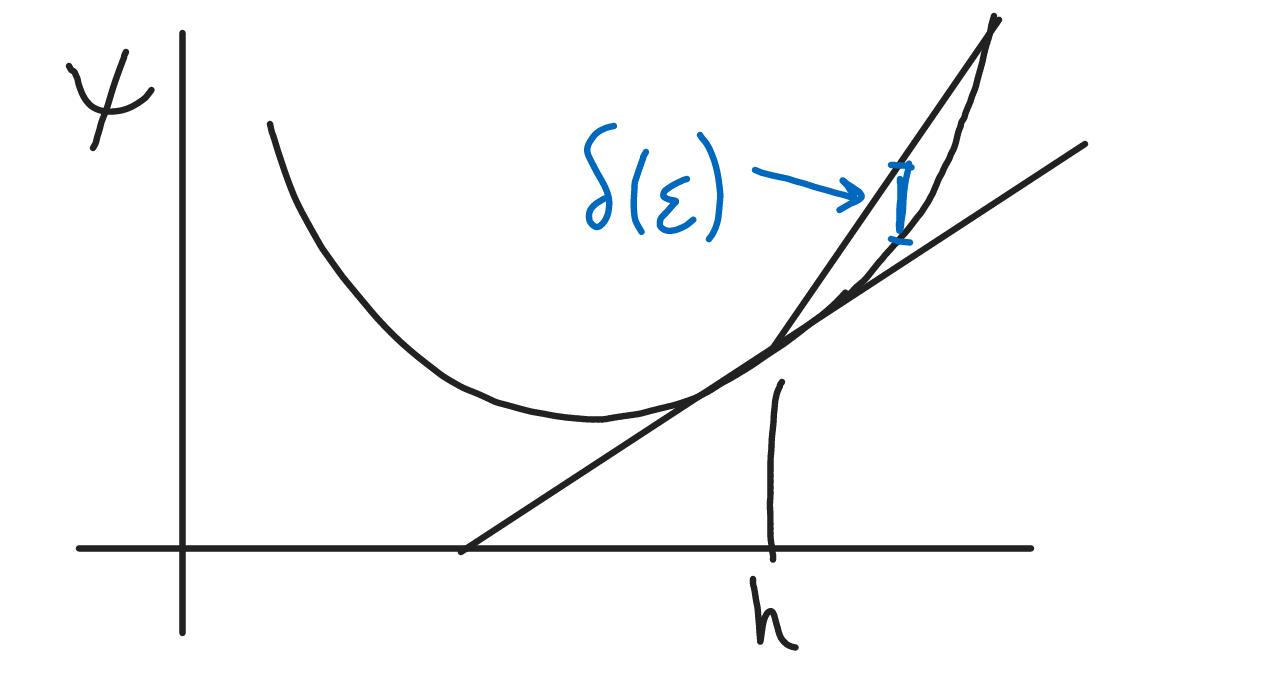
\includegraphics[scale=.25]{images/9-1}\end{center}

The probability that the energy density falls by $\varepsilon$ below its mean decays exponentially. This is the kind of decay we were talking about with large deviation principles.
Similarly we can show 
\be
\mathbb{P}_\beta (H\ge \left\langle {H}\right\rangle + \varepsilon|\Lambda|) \le e^{-\delta_+ (\varepsilon)|\Lambda|}.
\ee
%kettle on the floor.
%kettle on the table
This is left as an argument. 
We can repeat the argument, or apply what we proved to a system where the Hamiltonian is the negative.

The convex functions converge to a convex function. %Since $f$ converges pointwise, we can conclude from the convexity of the limiting function, 
%finite vs. infinite systems not so obvious. 
In the infinite volume limit, the function may not be differentiable, but the left and right derivatives exist. Our argument is really comparing with the slope of the function coming from above; for the other inequality, compare with the slope of the function from below.

Since the pressure converges, 
%REC
you can conclude that given a van Hove sequence, for $\Lambda$ large enough, you can conclude the bounds (not optimally) with $\delta/2$. 

\subsection{Large deviation principle for van Hove sequences}

\begin{theorem}
Assume that the infinite volume pressure $\psi$ is differentiable at $\beta_0$. Then for all $\Lambda_n\uparrow \mathbb{Z}^d$ (in the van Hove sense). %don't have to be cubes. suface-to-volume goes to 0.
Then for any $\varepsilon$, there is $N<\infty$ such that for all $n\ge N$, 
\be
\mathbb{P}_{\beta, \Lambda_n}\left( {\left| {\frac{1}{|\Lambda|}H_\Lambda(\sigma) + \psi'(\beta)} \right|\ge \varepsilon} \right)\le e^{-\frac{\delta(\varepsilon)}{2}|\Lambda|}.
\ee
\end{theorem}
If the infinite volume pressure is differentiable at a particular $\beta$, then in large enough finite volume, then the fluctuations per volume is small. with high probability. 
%corridor of small width, eventually finite volume pressures with $\ep$ of that. Half of that gap is realized. $\de(\ep)$ is read from the infinite value limit function. 
Look at the infinite volume function; for every $\varepsilon$, ask when we move right (left) at $\varepsilon$ greater (less) than the slope, how far we move to have the largest discrepancy. Wait for the gap between the infinite and finite volume case function to be less than half. 

So far we studied the distribution of the energy. But you may want to know the distribution of other quantities such as magnetization, spin, and number of clusters of a certain class. These are covered by the same analysis except you consider the dependence of the free energy. 

{\color{red}TODO: edit}
What is the physical implication for a lattice model? If you know the pressure as a function of inverse temperature. Pressure is a thermodynamic function. We are interested in sysm of deg ... tell us something... typical range of values of the energy of this configuration. At places where the energy is differentiable, the total energy per unit volume does not fluctuate much. We expect $\sqrt{}$ volume of fluctuations. This is like CLT for nonindependent variables.
%tiny $\ep$ times the volume. 
%REC


What happens if the pressure is not differentiable?
Without assuming differentiability of $\psi(\beta)$, we have 
\begin{align*}
\mathbb{P}_{\beta,\Lambda} \left( {\frac{1}{|\Lambda|} H \ge \psi'(\beta+0) + \varepsilon} \right)&\le e^{-\frac{\delta(\varepsilon)}{2}|\Lambda|}\\
\mathbb{P}_{\beta,\Lambda} \left( {\frac{1}{|\Lambda|} H \le  \psi'(\beta-0) -\varepsilon} \right) &\le e^{-\frac{\delta(\varepsilon)}{2}|\Lambda|}.
\end{align*}
(Note $\psi'(\beta-0)\le \psi'(\beta+0)$.) To extend to the densities of other local observables,
\be
H(\sigma) = \sum_{A\subseteq \mathbb{Z}^d} J_A \phi_A(\sigma)
\ee
with $J_A = J_{S_n}A$ for all shifts $S_n$. 
(The proper way to do this is to introduce coupling constants depending on the equivalence class of terms modulo translation. For example, Ising coupling has 2 parameters corresponding to nearest neighbor coupling and external field.)

For a collection of translation-invariant interactions, we denote 
\be
\psi(\beta,J) = \lim_{\lambda \uparrow \mathbb{Z}^d} \frac{1}{|\Lambda|} \ln Z_{\Lambda}(J,\phi).
\ee
\begin{theorem}\label{thm:j-limit}
For any translation-invariant interaction with $\left\Vert {J}\right\Vert<\infty$, %$\phi$ with $\ve{\phi}<\iy$, 
the limit 
$
\psi(\beta, J) 
$
exists and is a convex function of $J$ (it is jointly convex in all parameters). 
\end{theorem}
We think of pressure as a function of both the temperature and parameters such as the magnetic field.
%notation is not consistent.
%Banach space notation...
For example, for $H=-J\sum_{\{x,y\},|x-y|=1} \sigma_x\sigma_y - h\sum_x \sigma_x$, %infinitely many terms but 2 paramters. 
$\psi$ is a function $\psi(\beta, J,h)$. We have
\be
\frac{\partial \psi_{\Lambda}}{\partial h} = \beta\left\langle { \frac{1}{|\Lambda|}\sum_{x\in A} \sigma_x}\right\rangle.
\ee
and
\begin{align*}
\psi_{\Lambda}(\beta, J, h) &= \frac{1}{|\Lambda|} \ln \int e^{\beta(J\sum_{\left\langle {x,y}\right\rangle} \sigma_x\sigma_y+ h\sum_{x\in A} \sigma_x)}\rho_0(d\sigma)\\
\psi(\beta,J) &= \lim_{\Lambda\uparrow \mathbb{Z}^d} \frac{1}{|\Lambda|}\ln Z_{\Lambda}(J\phi)
\end{align*}
%jointly convex is almost everywhere diffble
%regardless whether continuous, can sandwich typical values within the left and right derivatives. 
%\begin{theorem}
%For any $\phi$ with $\ve{\phi}<\iy$, $\psi(\be,J)$ is jointly convex in $J$.
%\end{theorem}
Introduce as many parameters as you think are relevant.

In the homework, you will look at the simplest system, ideal gas. There are no interactions. We introduce something akin to the magnetization. Compute the pressure for an ideal gas and use this to compute the entropy of the system. The Legendre transform allows you to read the ... from the free energy. You'll learn how to arrive at this celebrated formula 
\be
-\rho\ln \rho + (1-\rho)\ln (1-\rho).
\ee
It becomes a challenge to evaluate partition functions and find their singularities. Ising calculated the partition function for the 1-D model; you will do the calculation too. He said it has no singularity. If you move to 2 dimensions, it does exhibit a phase transition. %Initial people we wrong.
The 2-D model is solvable by other techniques.
{\color{blue}3-1: First, notational adjustments}

Let
\begin{align*}
H_\Lambda(\sigma)&=\sum_{A\subseteq \Lambda} J_A\phi_A(\sigma)
\end{align*}
and assume $\phi$ is normalized so that 
\be
\sup_\sigma |\phi_A(\sigma)|  = 1
\ee
(if it is not identically 0). For $J=\{1_A\}$, define 
\be
\left\Vert {J}\right\Vert = \sum_{A\ni 0} \frac{1}{|A|} |J_A|.
\ee
\begin{definition}
$H$ is translation invariant if for all $A\subseteq \Lambda$,
\begin{enumerate}
\item
(Coupling is translation covariant)
$\phi_{A+u}(\sigma) = \phi_A(S_u\sigma)$, where $(S_u\sigma)_x = \sigma_{x+u}$. 
\item
$J_A=J_{A+u}$.
\end{enumerate}
\end{definition}
Note that $\phi$ is really ``shift covariant" whereas $H$ is ``shift invariant", i.e. $H(S_n\sigma) = H(\sigma)$ (formally). This is a formal expression because for an infinite system, the energy is infinite. (There are various ways to make sense of this mathematically. For example, you can look at a finite system with periodic bounary conditions, and we can talk about shift invariance there.)

For translation invariant Hamiltonians,
\begin{align*}
\psi(\beta, J) &=\lim_{\Lambda \uparrow \mathbb{Z}^d} \frac{1}{|\Lambda|} \ln Z_{\Lambda} (\beta, J))
%a priori measure
%try to stick to prob measures
%product measure
\end{align*}
where $Z_{\Lambda}(\beta, J) = \int_{\Omega_\Lambda} e^{-\beta H_{\Lambda}(\beta)}\rho_0(d\sigma_{\Lambda})$.

We proved 2 theorems, Theorem~\ref{thm:j-limit} and the following.
Let $h$ be one of the parameters of $J=\{J_\Lambda\}$ and $M$ be the conjugate quantity 
\beM_\Lambda(\sigma) = -\frac{\partial}{\partial h} H_{\Lambda}(\beta, J).\ee
\beM_\Lambda(\sigma) = -\frac{\partial}{\partial h} H_{\Lambda}(\beta, J).\ee
The example to keep in mind is the following.
%when you differentiate the hamiltonian

\begin{example}
The Ising model is $H_{\Lambda}(\sigma) =\sum_{\{x,y\}} J_{x-y}\sigma_x\sigma_u - h\sum_{x\in \Lambda }\sigma_x$.
Here, 
\be
-\frac{\partial}{\partial H_\Lambda(\sigma)}{\partial h} = \sigma_{x\in \Lambda}\sigma_x\equiv M.
\ee
\end{example}
We have $\frac{1}{|\Lambda|} \mathbb{E}(M_{\Lambda}) = \frac{1}{\beta} \frac{\partial}{\partial h} \psi$.
\begin{theorem}
For any $(\beta, J)$, for $\varepsilon>0$, there exists $\delta(\varepsilon)>0$ such that for any van Hove sequence, 
\be\lim_{\Lambda \uparrow \mathbb{Z}^d} \frac{1}{|\Lambda|}
\ln \mathbb{P}_{\Lambda}
\begin{pmatrix}
{
\frac{1}{|\Lambda|} M_{\Lambda}(\sigma) \ge \frac{1}{\beta} \left.\frac{\partial}{\partial h} \psi\right|_{+0} + \varepsilon\text{ or}
}\\
{
\frac{1}{|\Lambda|} M_{\Lambda}(\sigma) \le \frac{1}{\beta} \left.\frac{\partial}{\partial h} \psi\right|_{-0} -\varepsilon
}
\end{pmatrix}\le -\delta(\varepsilon)
\ee
\end{theorem}

This says that
%usually diffble
\be
\mathbb{P}_{\Lambda} \left( {\frac{1}{|\Lambda|}M_{\Lambda} \ge \frac{\partial}{\partial \psi}h + \varepsilon} \right) \approx e^{-\delta(\varepsilon)|\Lambda|}.
\ee
%max depth of belly is $\de(\ep)$. High $\ep$, high belly.

\section{1-D Ising model}
Consider the 1-D Ising model. The spins are $\sigma_n=\pm 1$; the energy is
\be
H(\sigma) = -J\sum_{n} \sigma_n\sigma_{n+1} - h\sum \sigma_n.
\ee
The first term encourages neighbors the agree, and the second term encourages the spins to agree with the applied field.
%solvable if limit to nearest neighbors

(Here we just have nearest-neighbor interactions. In general we can have interactions between longer distances, which complicates the calculations. When there are long-range interactions (following a power law), there can be a phase transition.)
%large - phase transition. power law, decay not too fast.
\begin{theorem}
Let $\widehat{h} = \beta h$. Then
\be
\psi(\beta, h):= \lim_{N\to \infty} \frac{1}{N} \ln Z_N = \ln [e^{\beta J} \cosh \widehat{h} + (e^{2\beta J} \sinh^2 \widehat{h} + e^{-2\beta})^{\frac{1}{2}}]
\ee
\end{theorem}
The particular form of the formula is not so important; what's important is that it is explicit. As a corollary, $\psi$ is differentiable at all $\beta \ge 0$, $h\in \mathbb{R}$ with 
\be
m(\beta, h):=\frac{\partial \psi}{\partial h} =  \frac{e^{\beta}\sinh \widehat{h}}{[e^{2\beta }\sinh^2 \widehat{h} + e^{-2\beta}]^{\frac{1}{2}}}
\ee
%arg of log is nonzero.
In particular, 
\be
\lim_{\beta\to \infty} m(\beta, h) = \begin{cases}
1,&h>0\\
0,&h=0\\
-1,&h<0.
\end{cases}
\ee
%story of the dog. did you notice strange behavior of dog. did not do anything, that's the point.
Note that we do not see the signature of a first-order phase transition, that the energy is discontinuous. The derivative is discontinuous, but the energy is not. We observe something like this only at infinite $\beta$. This is a general feature of 1-D statistical mechanical models: there is no symmetry breaking unless the model has very long-range interactions.

\begin{center}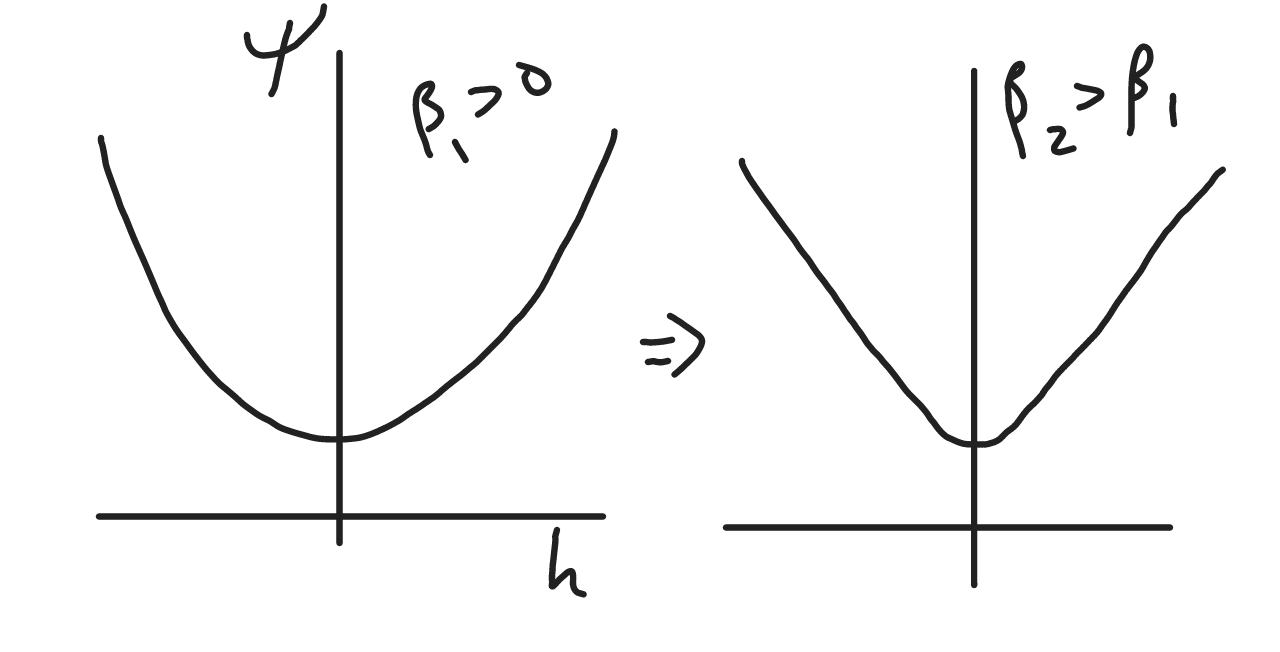
\includegraphics[scale=.25]{images/9-2}\end{center}

\begin{center}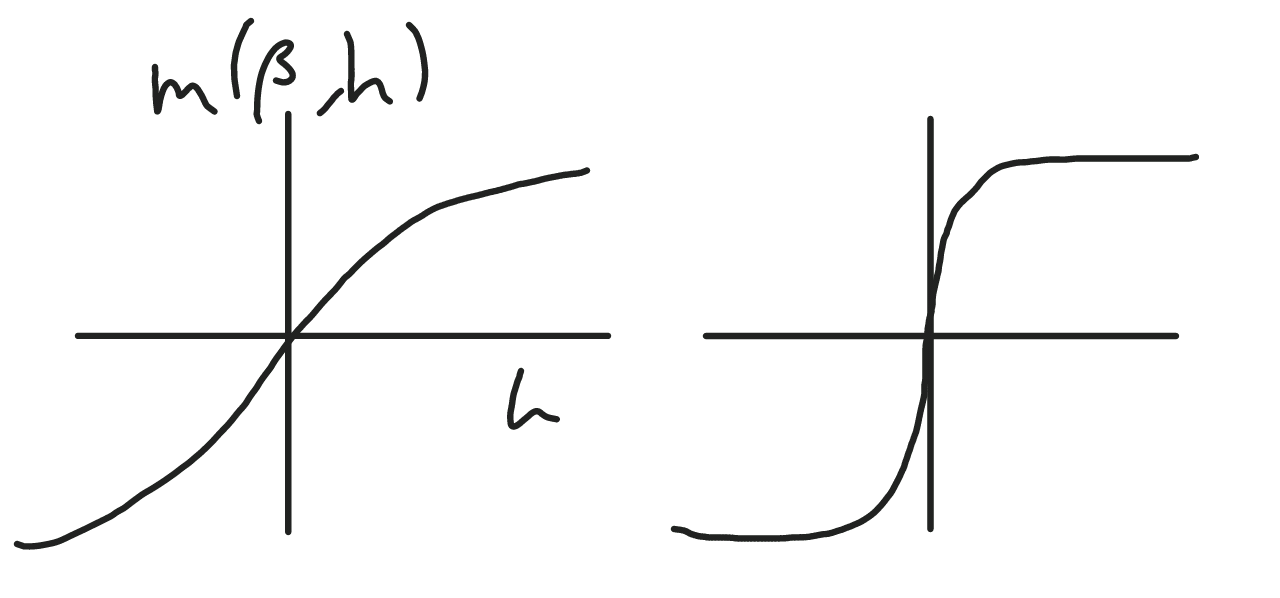
\includegraphics[scale=.25]{images/9-3}\end{center}

\begin{proof}
Take an Ising model with periodic boundary conditions $\sigma_L=\sigma_0$.
%sometimes parity matters sometimes not. Here it doesn't. 
Then (it helps to symmetrize the sum)
\begin{align*}
Z_{[0,L]}^{\text{per}} &= \sum_{\scriptsize \begin{array}{c}{\sigma_j=\pm 1}\\{\sigma_0=\sigma_L}\end{array}} e^{\beta \sum_{m=1}^L \sigma_m\sigma_{m+1} + \widehat{h} \sum_{1=1}^{L} \frac{\sigma_n+\sigma_{n+1}}{2}}\\
&=\text{tr} (A^L)
\end{align*}
where 
\be
A = 
\begin{pmatrix}
{A_{++}}&{A_{+-}}\\
{A_{-+}}&{A_{--}}
\end{pmatrix}
 = 
\begin{pmatrix}
{e^{\beta + \widehat{h}}}&{e^{-\beta}}\\
{e^{-\beta}}&{e^{\beta - \widehat{h}}}
\end{pmatrix}
.
\ee
Recall that 
\be
\text{tr}(A^L) = \sum_{\sigma_0=\sigma_L\in \pm 1} (A^L)_{\sigma_0\sigma_L} = \sum_{\scriptsize \begin{array}{c}{\sigma_i=\pm 1}\\{\sigma_0=\sigma_L}\end{array}} A_{\sigma_0,\sigma_1}A_{\sigma_1,\sigma_2}\cdots A_{\sigma_{L-1},\sigma_0}.
\ee
Since $A$ is self-adjoint, $A$ is diagonalizable. The eigenvalues have different modulus, $|\lambda_1|>|\lambda_2|$, and
\begin{align*}
\text{Tr}(A^L) &= \lambda_1^L +\lambda_2^L = \lambda_1^L\left[ {1+\left( {\frac{\lambda_2}{\lambda_1}} \right)^L} \right]\\
\frac{1}{L} \ln Z_L &= \ln \lambda_1 + \underbrace{\frac{1}{L} \ln \left[ {1+\left( {\frac{\lambda_2}{\lambda_1}} \right)^L} \right]}_{\approx \frac{1}{L}\left( {\frac{\lambda_2}{\lambda_1}} \right)^L}&\text{using }\ln (1+\varepsilon)\approx \varepsilon.\\
\lim_{L\to \infty} \frac{1}{L} \ln Z_L &=\ln \lambda_1 
%goes to 0 exp fast
\end{align*}
%if same, then identity. In modulus are not the same.
%$\la_2$ positive?

The matrix $A$ is a \index{transfer matrix}\textbf{transfer matrix} (as in a Markov chain). 
%pressure independent of boundary conditions. 
Fixing the boundary conditions $\sigma_0,\sigma_L$, we have
\be
Z_L^{b.c.} = \sum A_{\sigma_0\sigma_1}A_{\sigma_1\sigma_2}\cdots A_{\sigma_{L-1}\sigma_L} = (A^L)_{\sigma_0\sigma_L}
\ee
(Exercise: write this in terms of the eigenvalues.)
%hit on head for disagreement
\end{proof}
Consider $Z_L^{++},Z_L^{+-},Z_L^{-+},Z_L^{--}$.
Assuming the magnetic field is positive ($h>0$), the maximum is $Z_L^{++}$; if $h<0$ then the maximum is $Z_L^{--}$. We have
\be
\left| {\frac{Z^{++}-Z^{--}}{Z^{++}}} \right| \le \left| {\frac{\lambda_2}{\lambda_1}} \right|^L
\ee

%if open-ended boundary conditions, can ask the following.
With open-ended boundary conditions, the spins are an array of variables with the Markov property. If you specify a spin, then the distribution of the future does not depend on the past beyond the value of the previous spin. Thus the values form a Markov chain, and the transfer matrix is familiar from the theory of Markov chains. 

What happens beyond 1 dimension? Then the Markov property re-emerges in an interesting way. When you talk about the distribution of a finite system, it's sufficient to give the spins at the boundary. 
There is a multidimensional Markov property, specified by boundary spins. %Limiting boundary distribution,
We will arrive at the theory of Gibbs states.
%what can you learn from therm dyn pressure from Gibbs states
{\color{blue}3-3-16}

\subsection{Transfer matrix method}

This method applies to any finite model in 1 dimension. Suppose the individual states are $\sigma=\pm1$, $\{\sigma_i\}_{i=0}^L$
%observing particular configurtion.
The probability of observing a particular configuration is %boundar configuration $\si=(\si_0,\si_L)$ can be factorized as follows, %(having boundary conditions means we specify $\si_0,\si_L$),
\begin{align}
\mathbb{P}_\beta^{b.c.}(\{\sigma_{\Lambda_L}\}) &= \frac{e^{-\beta H_L^{bc}(\sigma)}}{Z_L^{br}(\beta)}\mathds{1}[\sigma_0,\sigma_L\text{ satisfy boundary conditions}]\\
\mathbb{P}_\beta(\sigma\text{ has boundary conditions } \sigma_0,\sigma_L)&=(T^L)_{\sigma_0,\sigma_L} \\
&= \sum_{\sigma =\{-1,1\}^{[1,L-1]}} T_{\sigma_0,\sigma_1}\cdots T_{\sigma_{L-1}\sigma_L}.
%how take matrix products.
\end{align}
Here, 
\begin{align}
T_{\sigma,\sigma'} &= e^{-\left[ {\beta J \sigma\sigma' + \widehat{h}\left( {\frac{\sigma+\sigma'}{2}} \right)} \right]}\\
&= e^{-\beta H(\sigma)} e^{\widehat{h}\left( {\frac{\sigma_0+\sigma_L}{2}} \right)}.
\end{align}
The product of these is
\be
e^{-\beta H(\sigma)} = e^{-\beta \sum_{j=0}^{L-1}\sigma_j\sigma_{j+1} - \widehat{h} \sum_{j=0}^L \sigma_j}.
\ee
%sum for each contraction?
%attractive nature, fluctuating spins which tend to be on the positive side. $\pm$ make a transition from one to another. 

%From $\si',\si$
%multiply get exactly Gibbs factor.
%pay attention to individual terms.
Another natural boundary condition is the periodic boundary conditions: we only allow states where $\sigma_0=\sigma_L$, so 
\be
Z_L^{\text{per}} = Z_L^{+,+}+Z_L^{-,-} = \text{Tr} (T^L).
\ee

\subsection{Markov chains}

We summarize some basic facts about Markov chains.
\begin{definition}
A $Q$-state \index{Markov chain}\textbf{Markov chain} is a collection of random variables $\{w_n\}$ with values in $[Q]=\{1,\ldots, Q\}$. Let $\Psi_n = 
\begin{pmatrix}
{P_n(1)}\\
{\vdots}\\
{P_n(Q)}
\end{pmatrix}
$ where $P_n(k) = \mathbb{P}(\omega_n=k)$.

$\Psi_1$ is in a given initial state\footnote{Probabilists use ``state" to mean the value of the random variable; physicists use ``states" to correspond to probability measure. (In quantum physics, not all variables have concrete values.)}, i.e., the probability distribution of $\omega_1$, and 
\be
\Psi_{n+1} = A\Psi_n
\ee
where $A_{ij}=\mathbb{P}(\omega_{n+1}|\omega_n=j)$ is \index{doubly stochastic}\textbf{doubly stochastic} $\sum_{j}A_{ij} = 1 = \sum_i A_{ij}$, $A_{ij}\ge 0$.\footnote{The LHS equality says that the Markov chain is reversible.}
\end{definition}
Think of $n$ as the discrete time.
Taking powers, we have
\be
\Psi_{n+1} = A^n \Psi_1.
\ee
%start with initial configuration and is propagated by a transition matrix.

Markov chains have finite memory; the effect of the initial value decays exponentially.
Nice Markov chains have a ``destiny" (equilibrium distribution). 
%arrow of time.
\footnote{The basic laws of physics seem reversible; how to explain the arrow of time? Consider colliding molecules; the impact parameters seem to be coming without precise aim in an uncorrelated way (Boltzmann's hypothesis), which isn't true if it is played in reverse. Entropy keeps increasing. Is there a moment when the entropy starts decreasing; does the arrow of time reverse?}
%arrow of time where 

A 1-D finite system looks like a Markov chain; boundary conditions are equivalent to specifying initial and final states.

\begin{theorem}[Perron-Frobenius]
Let $A=(a_{ij})$ be a $Q\times Q$ positive matrix $a_{ij}\ge 0$. 
\begin{enumerate}
\item
There is a positive eigenvalue $r$ (the Perron-Frobenius eigenvalue) such that the spectral radius of $A$ is $\rho(A)=r$ and $A$ has no other eigenvalue with $|\alpha|=r$.
\item
This eigenvalue is simple, and the corresponding eigenvector is positive.
\item Letting $|{v}\rangle$, $\langle{w}|$ be the left and right eigenvectors of $A$ corresponding to the largest eigenvalue, $A|{v}\rangle=r|{v}\rangle, \langle{w}| = r \langle{w}|$,
\footnote{We use Dirac's notation $|{v}\rangle=v^T$, $\langle{w}|=w$.}
\be
\lim_{L\to \infty} \frac{1}{r^L}A^L = |{v}\rangle\langle{w}|
\ee
\end{enumerate}
\end{theorem}
In other words, there is $S$ such that 
\beS^{-1}AS\approx r^L\begin{pmatrix}
1&0&\cdots\\
0&0&\cdots\\
\vdots &\vdots &\ddots
\end{pmatrix}.\ee
Applying this to the 1-D Ising model,
\begin{align}
Z^{\text{per}} &=
\sum_{j=1}^{Q} \lambda_j^L\\
& \approx \lambda_{\max}^L \left( {1+\left| {\frac{\lambda_2}{\lambda_1}} \right|^L +\cdots} \right)
%if you take the ising model, in the infinite volume limit the state exhibits exponential decay of correlations.
\end{align}
where 
\be
1>\left| {\frac{\lambda_2}{\lambda_1}} \right| = e^{-\delta}
\ee
where $\delta\lambda>0$ is the spectral gap, the gap between $\lambda_{\max}$ and the next smaller eigenvalue (in absolute value).
Using this, it is an exercise to show that in the Ising model, in the infinite volume limit the state exhibits exponential decay of correlations,
\be
\lim_{L\to \infty} \left| {\left\langle {\sigma_x,\sigma_y}\right\rangle_{[-L,L]}} \right| \le Ae^{-\delta |x-y|},
\ee
where $\left\langle {A,B}\right\rangle=\left\langle {AB}\right\rangle-\left\langle {A}\right\rangle\left\langle {B}\right\rangle$ is the covariance.
In the 1-D Ising model,
\be
\Psi(\beta,h)=\lim_{L\to \infty} \frac{1}{L}Z_L= \ln \lambda_{\max},
\ee
where $\lambda_{\max}$ is the Perron-Frobenius eigenvalue of $T=
\begin{pmatrix}
{e^{\beta+\widehat{h}}}&{e^{-\beta}}\\
{e^{-\beta}}&{e^{\beta-\widehat{h}}}
\end{pmatrix}
$.

The matrix elements are analytic. Can we conclude from this the analyticity of eigenvalues? They are when they don't bump into each other. When they do, funny things can happen. But here, Perron-Frobenius tells us that eigenvalues will not be equal (all entries in $T$ are positive). Thus the eigenvalues will be differentiable in $\beta,h$ and there is no phase transition.

\section{2-D Ising model}

Studying the transfer matrix going up, certain models are integrable; you can get a formula for the partition function. We'll present a different method which is culturally very important.
%early on in their career see solution of 3d 
%many careers were lost.
There is no closed-form solution in 3-D.

In contrast to the 1-dimensional case, in 2 dimensions, the free energy is not differentiable. 

Next we will show that for the 2D Ising model, for $\beta$ large enough ($\beta>\beta_c$) there exists $m(\beta)>0$ such that 
\begin{align}
\mathbb{P}_{\beta,k=0}^+\left( {\frac{1}{|\Lambda_L|}\sum_{x\in \Lambda_L} \sigma_x m\ge\frac{m}{2}} \right)&\to 1\\
\mathbb{P}_{\beta,k=0}^-\left( {\frac{1}{|\Lambda_L|}\sum_{x\in \Lambda_L} \sigma_x m\le \frac{m}{2}} \right)&\to 1
\end{align}
as $L\to \infty$. This indicates a phase transition. 
The signature of a phase transition is that when you take $\beta>\beta_c$, $h=0$ (so the Hamiltonian is invariant under spin-flip).
%in principle, true.

The Hamiltonian is $H=-\sum_{x,y\text{ neighbors}} \sigma_x\sigma_y$.
With $+$ boundary conditions, the spins are overwhelmingly positive. With $-$ boundary conditions, the spins are overwhelmingly negative. The system deep inside remembers the boundary conditions. 
Locally, there is symmetry; globally we have symmetry breaking.

What if we take symmetric boundary conditions, with $+$'s and $-$'s? Since it is invariant under a reflection, the probability of observing $\ge \frac{m}{2}+\varepsilon$ vanishes exponentially. The system organizes itself as follows: close to the $+/-$ boundary there is mostly $+/-$ with islands of $-/+$; in between there is an interface.

%There is a discontinuity
%We show that $\an{\si_x}$ is sandwiched between the left and right derivatives, $\an{\si_x}=-\pdd{h}\Psi$.

We will see Peiech's argument (?).


{\color{blue}3-8}

Peiech showed that these models can exhibit symmetry breaking.

In the 2-D Ising model, 
\be
H=-J\sum_{\{x,y\}} \sigma_x\sigma_y - h\sum_x \sigma_x.
\ee
\begin{theorem}[Peiech]
For the 2D nonnegative Ising model, there exists $\beta_0<\infty$ such that for $\beta>\beta_0$, at $h=0$,
\begin{align*}
\left\langle {\sigma_x}\right\rangle_{\Lambda,\beta,0}^+ &\ge m(\beta)\\
\left\langle {\sigma_x}\right\rangle_{\Lambda,\beta,0}^- & \le -m(\beta).
\end{align*}
with some $m(\beta)>0$. 
\end{theorem}
Why is this ``symmetry breaking"? If you take the model at external field $h=0$ (so that the measure is invariant under global spin flip), the expected value of any anti-symmetric quantity like spin is 0. If you put $+$ boundary conditions all around, then you expect there to be more $+$'s.  
More surprisingly, if you fix \emph{any} spin, even if the spins are far away, the bias persists.
%The place where you are furthest is 0, so it suffices to prove for that.

The theorem implies by linearity
\be
\left\langle {\frac{1}{|\Lambda|} \sum_{x\in \Lambda} \sigma_x}\right\rangle^+ \ge m(\beta).
\ee
Taking the van Hove limit,
\begin{align*}
\frac{\partial}{\partial h} \Psi(\beta,0+) & = \lim_{\Lambda\Uparrow \mathbb{Z}^2} \left\langle {\frac{1}{|\Lambda|} \sum_{x\in \Lambda} \sigma_x}\right\rangle^+ \ge m(\beta)\\
\frac{\partial}{\partial h} \Psi(\beta,0-)& = \lim_{\Lambda\Uparrow \mathbb{Z}^2} \left\langle {\frac{1}{|\Lambda|} \sum_{x\in \Lambda} \sigma_x}\right\rangle^- \le - m(\beta).
\end{align*}
%derivative at zero
Thus the left and right derivatives of $\Psi$ are unequal. There is a cusp at 0; there is a phase transition.

The theorem shows there is an asymmetry in the infinite volume limit of magnetization at a site.

For each $\sigma_{\Lambda}\in \Omega_\Lambda$ draw a green line separating $+/-$ spins. 
Using
\be\sigma_x\sigma_y = 2\mathds{1}[\sigma_x=\sigma_y]-1\ee
(this takes $\pm1$ values). 
We have
\begin{align*}
e^{-\beta H(0)}&=\prod_{\{x,y\}} e^{\beta \sigma_x\sigma_y} = e^{\beta|\xi|} \prod_{\{x,y\}}  e^{-2\beta \mathds{1}[\sigma_x\ne \sigma_y]} = K e^{-2\beta|C|}
\end{align*}
where $K$ is a constant and $C$ is the set of contour lines.

%suppressed by $e^{-2\be}$ times the number of lines.
%loops cost energy. excitation.
%hamiltonian. What is the energetically most favorable thing to do?
%particles of the model...

If the boundary conditions are $+$, then for there to be a $-$, it must be separated from the boundary by a green loop. We want to show that the probability for a given site to be separated from the boundary by a loop is strictly less than $\frac{1}{2}$. Then the probability it agrees with the boundary is $>\frac{1}{2}$.

Let $\Omega_{\gamma}$ be the set of configurations which has $\gamma$ as a contour.
\begin{lemma}[Peiech]
The probability that a given loop $\gamma$ is among the contours lines $C(\sigma)$ satisfies
\be
\mathbb{P}_{\Lambda,\beta,0}^+(C(\sigma) \ni \gamma )= \left\langle {\mathds{1}_{\Omega_{\gamma}}}\right\rangle^+_{\Lambda,\beta,0}\le e^{-2\beta |\gamma|}.
\ee
\end{lemma}
\begin{proof}
First we do an energy estimate.

The idea is that each configuration can be associated with another configuration by a mapping $T_\gamma$ which flips the spin of all sites inside $\gamma$. The disagreements of $\gamma$ would be erased. Because all spins inside are flipped, no other disagreement is affected. Note $T_\gamma$ is an involution---it is its own inverse.
%takes out of set in invertible way. 
%consider mapping which flips the spin. disagreement would be erased, all inside is flipped, so no other disagreement is affected.

For each $\sigma\in \Omega_{\gamma}$, its flip has higher probability because it has less disagreement, so
\be
\mathbb{P}^+(\{\sigma\}) = e^{-2\beta |\gamma|} \mathbb{P}(\{T_\gamma\sigma\})%\le e^{-2\be |\ga}.
\ee
Summing over $\sigma\in \Omega_{\gamma}$,
\be
\mathbb{P}^+(\Omega_{\gamma}) = e^{-2\beta |\gamma|} \mathbb{P}(T_\gamma\Omega_{\gamma}) \le e^{-2\beta |\gamma}.
\ee
%For each $\si\in \Om_{\ga}$, 
%\be
%\Pj^+(\{\si})\le
%\fc{\Pj^+(\{\si\})}{\Pj(\{T_\ga\si\})+\Pj(\{\si\})} 
%= \fc{e^{-2\be |\ga|}}{1+e^{-2\be |\ga|}} \le 2^{-2\be|\ga|}.
%\ee
%winning one mi

Next we need an entropy estimate: we need to estimate how many loops there are so we can do a union bound over them.
\begin{lemma}[Entropy estimate]
The number of non-repeating loops of length $l$ starting from a specified point is $N_l\le \frac{4}{3}3^l$.
\end{lemma}
\begin{proof}
There are 4 possibilities for the first step; for each of the next step there are $\le3$ choices for the other $l-1$ steps because it can't backtrack.
\end{proof}

Now we put the energy and entropy bound together.
For each each loop around $x$, we can start it at an node between 0 and $\frac{l}{2}$ steps to the right of $x$ where the path goes up. Then %  Choosing the first step to be up in the path
\begin{align*}
\mathbb{P}^+(\sigma_x=-1) &\le \mathbb{P}^+\left( \text{$x$ is separated from $\partial \Lambda$} \right)\\ 
&\le \sum_{\gamma\text{ loop separating $x$ from $\partial \Lambda$}} e^{-2\beta |\gamma|}\\
&\le \sum_{l=4}^{\infty} \frac{l}{2} 3^{l-1} e^{-2\beta l}\\
&=\frac{1}{6} \sum_{l=4}^{\infty} l(3e^{-2\beta})^l.
\end{align*}
This is $\le \frac{1}{2} - \delta(\beta)$ for $\beta>\beta_0$ where  $\beta_0$ is defined by the condition
\be
\frac{1}{6} \sum_{l=4}^{\infty} l (3e^{-\beta_0})^l = \frac{1}{2}.
\ee
%number of choices.
%how unlikely for a given contour to happen.
\end{proof}
The condition is ugly. With some extra finesse, we can show $3e^{-\beta}<1$ is sufficient for there to be symmetry breaking.

This implies that for $\beta>\beta_0$
\be
\left\langle {\sigma_0}\right\rangle_{\mathbb{Z}^2}^+=\lim_{\Lambda \Uparrow \mathbb{Z}^2} \left\langle {\sigma_0}\right\rangle_{\Lambda,\beta,0}^+ \ge m(\beta)>0.
%local quantity with _ boundary conditions.
%prob dist of measure
\ee
Here we define an infinite volume probability distribution by taking the limit of finite probability distributions with $+$ boundary conditions.   Similarly define $\left\langle {\sigma_0}\right\rangle_{\mathbb{Z}^2}^-$. Symmetry breaking refers to the fact that
\be
\left\langle {\sigma_0}\right\rangle_{\mathbb{Z}^2}^+\ne \left\langle {\sigma_0}\right\rangle_{\mathbb{Z}^2}^-.
\ee

Consider a function $G(m)=G(-m)$. If $G$ has the symmetry of the variational problem, the minimum is at 0.
%In symmetry breaking the minimum is not at 0. %: the solution of the variational problem. 
If the minimum does not have the symmetry of the variational problem, there may be multiple minima. We refer to this as symmetry breaking.

\begin{remark}
One can deduce symmetry breaking already for $\beta>\beta_1$ with $\beta$ defined by $3e^{-2\beta_1}=1$. 

Actually we're counting self-avoiding walks; the rate that they grow is smaller than $3^l$. So we can replace 3 by the actual rate; this is more complicated. It's harder to come up with exact values.
\end{remark}
%Convergence gives symmetry breaking.

The part of the estimate which is not relevant is short loops. Let's look at a larger scale and only count loops which surround a larger box. If the probability of there being a large loop around $x$ is $<\frac{1}{2}$, then we can already conclude symmetry breaking. For $3e^{-2\beta}<1$, we can choose $l$ large enough so that this holds.

If the box of size $n$ is not surrounded by a loop, we can conclude there exists some loop of $+$ spins outside the box which is connected to the boundary. %encircling the box of size $n$. 
This event is not compatible with the flip of the event. Thus the probability that there is a loop of $-$'s of size $>n$ connected to the boundary (with $-$) is $<\frac{1}{2}$.

In the infinite volume case, we cannot both have a loop connected to $\infty$ with $-$'s and a loop connected to $\infty$ with $+$'s. The $+$ event is more likely.

If you start with $+$ boundary conditions, the $+$ case will occur with large probability.

There is percolation of $+$ sites. If there is no symmetry breaking, there is percolation of $-$ sites. You have to work to show that you can't have infinite line of $+$'s and infinite line of $-$'s with nonzero probability  %In our case, both cannot occur simultaneously. %choke line of 
Harris developed the theory of this. We take a shortcut and show that a stronger condition (with the ring of $+/-$'s) is incompatible.

%We take shortcuts. 
%estimates do not squeeze most.
When you take this approach, there are 2 special values of the parameters: a $\beta$ for which we get no information (the sum diverges), and the $\beta$ for which the sum is less than a certain threshold ($\frac{1}{2}$). Looking at a renormalized version which eliminates the noise from the low cases of the sum, and you can improve the $\beta$ threshold.

In higher dimensions, you have to enumerate surfaces. The energy bound is easy. The energy (enumerating surfaces) is messier. The entropy estimate gives worse bounds. You have to be clever to bring other techniques.

Another way is to take the restriction to 2 dimensions (a slice of the cube). If you decouple the layers you just get the 2D model. Having other spins around only increases cooperations. 
%clusters of cooperation
%connected to floors above and below.
This brings us to the use of inequalities. For the 3D model, the magnetization is greater than the 2D model for the same temperature. 

With appropriate inequalities one can show
\be
\left\langle {\sigma_0}\right\rangle_{[-L,L]^3}^+\ge \left\langle {\sigma_0}\right\rangle_{[-L,L]}^+.
\ee
This implies symmetry breaking in higher dimensions at the same temperature, so the critical temperature is smaller,
\be
\beta_{c}^{3D} \le \beta_c^{2D}.
\ee
Here
\be
\beta_c = \inf \left\{{\beta}:{\left\langle {\sigma_0}\right\rangle_{\beta'}>0 \forall \beta'>\beta}\right\}.
\ee
For 2 dimensions, $\beta_c$ is calculable; for 3 dimensions we don't have an exact value. The 2-D Ising model is exactly solvable by a nontrivial argument. We'll present Feynman's solution.
%There is a discontinuity in the spontaneous ... across this line.

How singular is the magnetization? That's not expected to change with local details, but with dimension. We do not know $\beta_c$ for range 5 Ising model, but we expect that the power of $m(\beta)$ is the same (it grows like a power function from the critical temperature).

{\color{blue}3-10: We continue the 2D Ising model. Much of what we say will hold true for other planar graphs. }

The energy is 
\be
\sum_{b\in \mathcal{E}}J_b (\sigma\sigma)_b - h\sum_{x\in G}\sigma_x
\ee 
where the first sum is over edges (bonds) and if $b=b_1b_2$, then $(\sigma\sum_{n=0}^{\infty})_b$ denotes $\sigma_{b_1}\sigma_{b_2}$.

The state changes discontinuously across the line $h=0$ until some critical temperature $T_c$. Along the symmetry line the model is solvable.
\begin{theorem}[Onsager]
For the nn $\mathbb{Z}^2$ at $h=0$, $J_b=J$, 
\be
\frac{1}{|\Lambda|} \ln Z_{\Lambda}^{\text{per}} (\beta, 0) = \ln \cosh (\beta J)
+ \frac{1}{2} \int_{(-\pi, \pi]^2} \frac{dx_1\,dx_2}{(2\pi)^2}\ln \left\{ {
\left[ {
Y(\beta) + Y^{-1}(\beta) - 2
} \right] + \mathcal{E}(k)
} \right\}
\ee
where $\mathcal{E}(k) = 2\left[ {\sin^2 \left( {\frac{k_1}{2}} \right) + \sin^2\left( {\frac{k_2}{2}} \right)} \right]$.

By the integral we really mean the discrete sum over $k\in (-\pi,\pi]^2 \cap \frac{2\pi}{L}\mathbb{Z}^2$. (In the infinite volume limit it is an integral.)
%elastic membrane.
\end{theorem}
%discrete momenta as sites in spce.
For square summable function in a box, we can look at a basis of delta functions, or the Fourier basis $e^{ik\cdot x}$ for $k\in (-\pi,\pi]^2 \cap \frac{2\pi}{L}\mathbb{Z}^2$. I.e., $k$ is sampled from the dual lattice; $[-\pi,\pi]$ is subdivided to have the right number of points.
%condensed matter physics. Fourier analysis.
%In many books where Onsager's theorem..., they stop short of this expression.

Note $\sinh$ is an unbounded monotone increasing function. 
%what $Y+Y^{-2}-2$ looks like: min 0 at 1.
%sum won't be both 0 if temperature is other than 0.
%At the critical temperature, $Y(\be)+Y^{-1}(\be)-2$ vanishes, and the singularities are those of $\cal E(k)$.

For $h=0, b\in \mathcal{E}(\mathcal{G})$,
\begin{align*}
Z_{\Lambda} &= \frac{1}{2^{|\Lambda|}} \sum_{\sigma \in \Omega_{\Lambda}} e^{-\beta H_{\Lambda}(\sigma)}\\
&\qquad e^{-\beta H(\sigma)} = e^{\sum_b (\sigma\sigma)_b \beta J_b} = \prod_b e^{\beta J_b (\sigma\sigma)_b}& \text{(factorizing over bonds)}\\
&=\frac{1}{2^{|\Lambda|}} \sum_{\sigma\in \Omega_{\Lambda}} \prod_b [\cosh(\beta J_b) + \sinh(\beta J_b)(\sigma\sigma)_b]&e^x = \cosh x + \sinh x\\
&=\left[ {\prod_b \cosh(\beta J_b)} \right] \frac{1}{2^{|\Lambda|}}\sum_{\sigma\in \Omega_{\Lambda}} \prod_b[1+K_b(\sigma\sigma)_b]&\text{where }K_b=\tanh(\beta J_b)\\
&=\left[ {\prod_b \cosh(\beta J_b)} \right] \mathop{\mathbb E}_{\sigma} \sum_{\Gamma\subseteq \mathcal{E}(\mathcal{G})}\prod_{b\in \Gamma}K_b \left( {\prod_{b=\{x,y\}\text{ in }\Gamma} (\sigma\sigma)_b} \right)\\ 
&=\left[ {\prod_b \cosh(\beta J_b)} \right] \sum_{\Gamma}\prod_{b\in \Gamma}K_b
\mathop{\mathbb E}_{\sigma} \left( {\prod_{b=\{x,y\}\text{ in }\Gamma} (\sigma\sigma)_b} \right)&\text{linearity of expectation}
\end{align*}
We expressed the sum in terms of the symmetric and anti-symmetric parts and pulled out a factor $\cosh$. 
%\fixme{Where $\Ga$...}
%Here $\Ga$ is over sets of loops (i.e., possibilities for the places where $(\si\si)_b=-1$).
%nmber of bonds contain a site x
%if single side for which this is an odd poewr, the average is 0.
%if the power is even for all spins, the averge is 1.
The average is easy to compute: if there is a spin for which the power is odd, the average is 0; if the power is even for all spins, the average is 1.
\be
\mathop{\mathbb E}_{\sigma} \left( {\prod_{b\in \Gamma} (\sigma\sigma)_b} \right) = \mathop{\mathbb E}_{\sigma}\prod_x \sigma_x^{\sum_{b\in \Gamma} \mathds{1} [b\ni x]}
= \mathds{1}[\forall x,(-1)^{\sum_{b\in \Gamma} \mathds{1}[b\ni x]}=1]
\ee
%good graph obtained from closing

%Factorize over bonds
%\bal
%e^{-\be H(\si)} &= e^{\sum_b (\si\si)_b \be J_b} = \prod_b e^{\be J_b (\si\si)_b}.
%\end{align*}
Let $(\partial \Gamma)_2=\left\{{x}:{x\text{ belongs to an odd number of edges}}\right\}$. The condition for the summand to not vanish is $(\partial \Gamma)_2=\phi$.

We summarize this calculation as a lemma.

%\begin{theorem}[Feynman-Sherman]
%
%\end{theorem}
%complexity not reduced yet.
\begin{lemma}
For $h=0$,
\begin{align*}
Z_\Lambda &= \left[ {\prod_b \cosh(\beta J_b)} \right] \sum_{\Gamma, (\partial \Gamma)_2=\phi} \prod_{b\in \Gamma}K_b.
\end{align*}
\end{lemma}

\begin{theorem}[Feynman-Sherman]
Let $K(\Lambda)= \prod_{b\in \Gamma} K_b$.
\be
\sum_{\Gamma:(\partial \Gamma)_2=\phi} K(\Gamma) =  \prod_{\text{loops}}[1+(-1)^{n(l)}K(l)]
\ee
where $n(l)$ is the number of self-intersections of $l$.
\end{theorem}
Each graph can be covered by a collection of loops (which can cross and repeat edges).
%completing loops
%start from RHS: double counting.
Note the RHS is an infinite sum. By a lot of identities this infinite sum reduces to a finite sum.

Kac-Ward introduced the Ihara zeta function.

The RHS is 
\begin{align*}
 \prod_{\text{loops}}[1+(-1)^{n(l)}K(l)] &= \sum_{m:\mathcal{E}(G) \to \mathbb{Z}_+} {\prod_b K_b^{m_b}} W(m)\\
\text{where }W(m) &= \sum_{\ell_1,\ldots} \prod_j (-1)^{n_{\ell_j}}\mathds{1}_m[\{\ell_1,\ldots, \ell_k\}].
\end{align*}

%how many times is each bond is visited by each loop of collection...
%when weights small enough, convergent infinite product
%how many ways edge is visited.

\begin{lemma}
If $\left\Vert {m}\right\Vert_{\infty}:=\max_b(m_b)=1$ then $W(m)=1$.
\end{lemma}
%If weights are 0 or 1 for all bonds, then the contribution of the RHS is 1. Sticking just with $W(m)=1$, this captures all partition functions.

Sum over the multisets of edges. We need to enumerate how many ways the multisets can be realized as a union of loops. 
The Katz-Ward idea is enumerate all the different ways to resolve the traffic jams at each vertex with an intersection: sum over all possible choices with the right signs. The other vertices don't present any choices for the prospective loop.

\begin{center}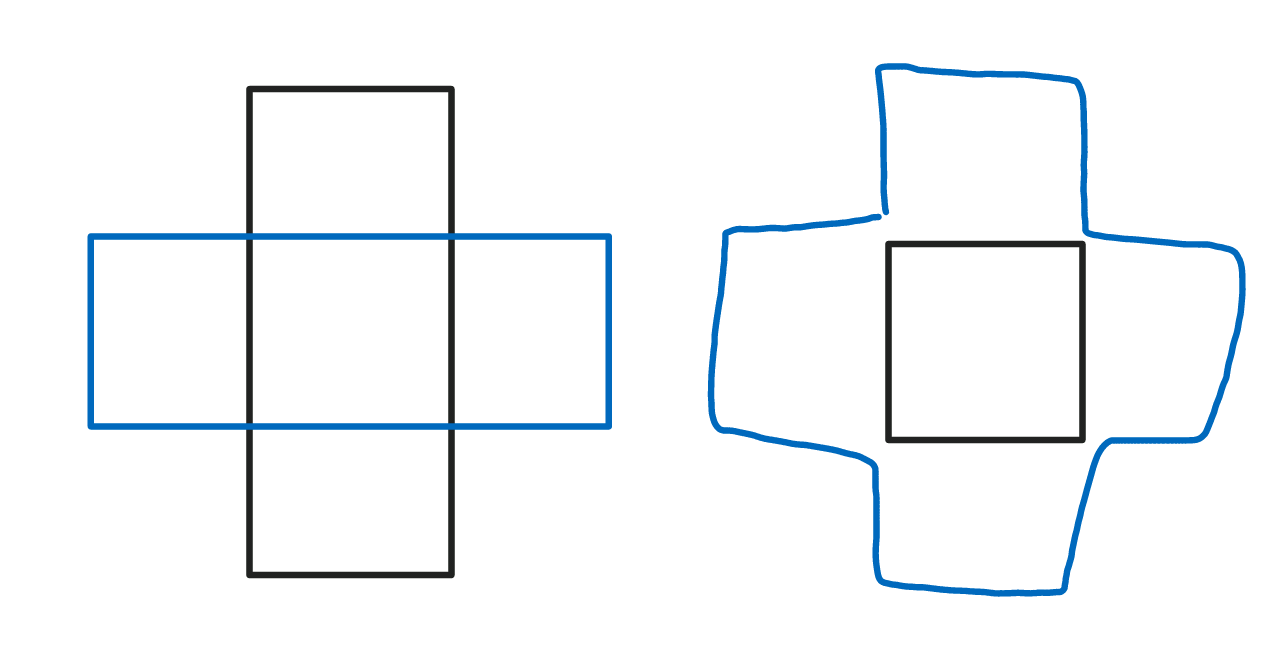
\includegraphics[scale=.25]{images/12-2}\end{center}

The three possibilities are:

\begin{center}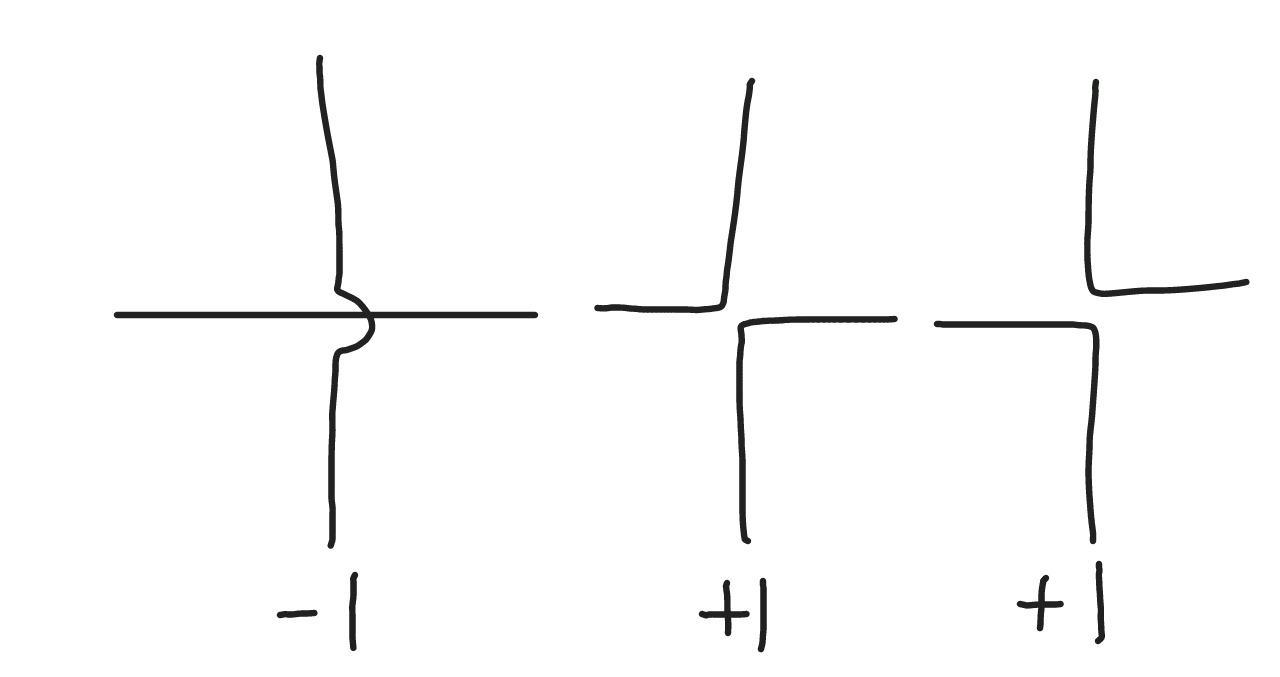
\includegraphics[scale=.25]{images/12-3}\end{center}

%The sum is 1.
%Think of loops as limits of continuous curves. It's not clear whether under magnification... the number of times curves cross each other.
The parity is certain. 
%the number of crossings disappear from view.
%deformation: disentangle wire.
%Whitney theorem. Intuitive things hard to prove.
%crossing of single curve with self or other. 
%Two curves always have an even number of intersections. (If you pull them apart, intersections will disappear in pairs.)

\begin{lemma}
If $\left\Vert {m}\right\Vert_{\infty}=2$ then $W=0$.
\end{lemma}
\begin{proof}
This means there is one edge traversed twice. Take one of these edges. How are the loops arranged in the complement? There are 2 possibilities for how the loops hook up through the bond. Summing you get 0.
\end{proof}
What if it's $>2$? This is in fact true for any value $>1$.

Why are the higher powers 0? %There are things like graph zeta functions.

\begin{theorem}[Sherman]\label{thm:sherman} %Kac-Wald, 
\be
\prod_{\text{loops}} [1+(-1)^{n(\ell)}K(\ell)]^2 = \det(\mathds{1} - \mathcal{L})
\ee
where $\mathcal{L}$ is a $2|\mathcal{E}|\times 2|\mathcal{E}|$ matrix indexed by the oriented edges. Here 
\be
\mathcal{L}_{e,e'} = \delta_{O(e'),t(e)} e^{\frac{i\angle(e,e')}{2}}K_e.
%$e$ to flow into $e'$.
\ee
(The Kronecker delta function says that $e$ has to flow into $e'$, i.e., the terminal of $e$ is the same as the origin of $e'$. Here $\angle(e,e')$ means the angle between $e,e'$. We get a phase number that's half the sum of the turns. For a simple loop, we get $-1$.)
\end{theorem}
$\text{Tr} \mathcal{L}^n = \sum_{e_1,\ldots, e_n} = \mathcal{L}_{e_1,e_n}\cdots \mathcal{L}_{e_2,e_1}$. This is associated to an oriented loop.
%n(\ell)$ self intersections.

%There's a general relation...
%Finite product expression for infinite product.
Buried in this is an infinite collection of relations. In principle we have contributions in the RHS of the theorem with arbitrarily many loops. But Sherman's theorem says that it is multilinear in the weights of the edges. Higher powers do not contribute. 

You can decompose the Hilbert space into Fourier modes. For each value of the momentum you have a finite-dimensional space. Edges are indexed by position and direction. If you change to momenta and direction, the different momenta are not mixed by shifting. The determinant is a block determinant where different values of the momenta are not mixed. We get $4\times 4$ blocks; the determinants can be computed and we get the solution.

{\color{blue}3-22}

We can use the transfer matrix method for 1D systems with finite range correlations (of distance $R$), not just nearest-neighbor interactions. Let the states be $\tau_x=\{(\sigma_x,\sigma_{x+1},\ldots, \sigma_{x+R})\}$. Switching to this space, we can now express the energy in terms of nearest neighbor interactions,
\be
H=\sum_n \Phi(\tau_n,\tau_{n+1}).
\ee

%aggregating some states.

\subsection{Ihara graph zeta function}

\begin{definition}
A \textbf{path} in a graph $\mathcal{G}$ is a set of edges $(x_1,x_2),\ldots, (x_n,x_{n+1})\in \mathcal{E}$. For an \textbf{oriented path}, the direction matters. In a \textbf{closed path}, $x_{n+1}=x_1$. An \textbf{oriented loop} is a closed oriented path where we don't care about the starting point, i.e., an equivalence class of paths modulo cyclic permutation. Two paths are equivalent here if $y_i=x_{i+h}$, with indices taken modulo $n$.

Edges are allowed to repeat.

For a path $p$, denote by $|p|$ the number of edges in $p$.
\end{definition}
We would like to eliminate paths which are powers of more elementary paths, complete repetitions of a primitive path. A path is primitive if it is not a power of a shorter path.

\begin{definition}
A path is \textbf{primitive} if it cannot be written as $q^k$, $k>1$, where $q$ is a closed path.
\end{definition}
This may remind you of prime numbers. Any number can be written as a product of numbers which cannot be decomposed. People applied number-theoretic ideas to graphs.
%People started thinking about number-theoretic

\begin{theorem}
Let $M$ be a matrix indexed by sites of a graph $\mathcal{G}$.
For $\left\Vert {M}\right\Vert$ small enough, %hen
\be
\det(\mathds{1}-M) = \prod_{p^{*}} [1-\chi_\mu(p)]
\ee
where the product is over equivalence classes $p^*$ of primitive oriented loops.
%matrix nonzero only for edges. don't hopscotch crazily.

Here 
\be
\chi_p=\prod_{n=1}^{|p|} M_{x_{n},x_{n+1}}.
\ee
\end{theorem}
%invar under cyclic reparametrization.

On the RHS, when we open the brackets, we can worry about convergence. For matrices of small norm, it is convergent. To define the function for all $\lambda$, note the theorem establishes that for small $\lambda$,
\be
\det(\mathds{1}-\lambda M) = \prod_{p^{*}} [1-\lambda \chi_\mu(p)].
\ee
Now we can take the analytic continuation.

Note the LHS is a finite calculation (and a multilinear function in entries of $M$), while the RHS is an infinite product/sum.

%mats with no loop
%for $\la$ small enough.

It follows from the proof that the RHS is a convergent product (for $\left\Vert {M}\right\Vert$ small enough).
\begin{proof}
First assume $\left\Vert {M}\right\Vert<1$. (This is the operator norm, $\left\Vert {M}\right\Vert=\max_v\frac{\left\Vert {Mv}\right\Vert}{\left\Vert {v}\right\Vert}$.) Then
\be
\ln \det(1-M)  = \text{tr}\ln (\mathds{1} -M).
\ee
For Hermitian matrices, prove this by diagonalization: the LHS is $\ln \prod_j (1-\lambda_j) = \sum_j \ln (1-\lambda_j)$. 

For the general case, we can still use this method. Write $M=S^{-1}TS$ where $T$ is upper triangular. If the diagonal entries are $\lambda_1,\ldots, \lambda_n$, the determinant is still $\prod_j(1-\lambda_j)$. 
%the only factor in the product is the diagonal.
%operator norm.

Expanding gives
\begin{align*}
\ln \det(\mathds{1}-M) &= -\sum_{n=1}^{\infty} \frac{1}{n} \text{tr}(M^n) \\
%&= -\sumo k{\iy} \sum_{p^*} \rc{k|p^*|} k \chi_n(p^*)^k
%elem enumeration for closed paths
%conribut at rate proportion to nmber of places where can start, total length / k.
&= \sum_{x = (x_0,\ldots, x_n)} \frac{1}{n} \left( {\prod_{j=1}^n M_{x_{j+1},x_j}} \right) \\
%&= \sumo k{\iy}\pa{\sum_{x\text{ primitive}}M_{x_{j+1},x_j}}}\\
%&= \sum_x \sumo k{\iy}
&=-\sum_{k=1}^{\infty}\sum_{p^*} \frac{1}{k|p^*|} \chi_M(p^*)^k\\
&=-\sum_{p^*} \ln (1-\chi_M(p^*)).
\end{align*}
$k$ comes from properly weighing the volume of the path.
%This is a sum over closed paths
\end{proof}

We want to avoid backtracking. %Think of $\cal L$
%\begin{theorem}
%Let $\cal E$ be the graph of oriented edges of $\cal G$.
%%backtracking and tadpoles
%%powers generate closed walks to avoid backtracking.
%
%\end{theorem}
\begin{thm*}[Theorem~\ref{thm:sherman}]
Let $\mathcal{E}$ be the graph of oriented edges of a planar graph. Let 
\begin{align*}
\mathcal{L}_{e,e'} = \mathds{1}[O(e')=t(e)]K_e e^{\frac{i\angle(e',e)}{2}}
\end{align*}
For any oriented closed path,
\begin{align*}
\prod_j \mathcal{L}_{e_j,e_{j+1}} = \prod_i K_e(-1)^{w(p)}
\end{align*}
%winding number.
with 
\be
(-1)^{w(p)} n= -(-1)^{n(p)}.
\ee
where $w(p)$ is the winding number and $n(p)$ is the number of crossings. 

\end{thm*}
%take 
%If cross sel, at that poit rerout to avoid the path
%reduces winding number of 2
We have
\begin{align*}
\prod_{p^*} [1-\chi_{\mathcal{L}}(p^*)] 
&=\sum_{\mathcal{P}= (p_1^*,\ldots, p_n^*)} \prod_j (-1)^{n(p_j)} k[p]\\
&=\sum_m\pi_e K_e^{m_e}W_m
%n?
%characterize by not thinking about the ... but the frequency of edges travesed.
%realized through collections of paths.
\end{align*}
where $W_m$ is the number of of paths with a given frequency of edges traversed. 

\begin{lemma}[Kac-Ward]
We have
\be
\sum_{P: \max_e(m(P))= 1} (-1)^{n(P)}K(P) = \sum_{\Gamma:\partial \Gamma = \phi} \prod_{e\in \Gamma} K_e = Z(\beta)
\ee
for $K_e=\tanh (\beta J_e)$. 
\end{lemma}

Each vertex has 3 possibilities.

{\color{blue}3/24/16}

Introduce $t=\frac{\beta-\beta_c}{\beta_c}$. 
What momenta contribute to the rise in the specific heat? That which $E$ is on the order of $Y+Y^{-1}-2$. Do some dimensional analysis. 

The specific heat is 
\be
C=\frac{\partial}{\partial T} \left\langle {H}\right\rangle_\beta = \beta^2\frac{\partial^2 }{\partial {\beta}^2}\Psi = \cdots \ln|\beta-\beta_c|+\cdots 
\ee

Certain fermionic structures pop up. We start from a classical system and out of that the excitations take the form of quantum objects, like quantum spinors (B Kaufman and Lee Scholz). This employed the 2D transfer matrix. When you try to solve it, you transfer from 1 layer to another; the dimension of the matrix is linearly proportional to $n$. In 2D, for reasons to do with integrable systems in 1D, the transfer matrix can be diagonalized. 


The loops we generate can have 1 edge multiple times. We have to disentangle the system of graphs which correspond to configurtions of loops. 

In a high dimension, loops typically miss each other. Perhaps Onsager's solutions may emerge in higher dimensions. (Dimension 3 is the hardest.)

Weight each loop by the product we want. 
%periodic orbit, multiply.



%The world is really quantum

{\color{blue}3-29-16}

\section{Gibbs states in the infinite volume limit}

Let $S$ be the set of spin states. $S$ is typically a compact space. For example, in the Ising/Potts spin models, $S=\{1,\ldots, Q\}\subset\mathbb{N}$. In the $O(n)$ spin models, $S=\left\{{\sigma\in \mathbb{R}^n}:{|\sigma|=1}\right\}$.\footnote{Note that physicists say that the sphere in $\mathbb{R}^n$ is $n$-dimensional, while mathematicians say it is ($n-1$)-dimensional.} Let $\mathcal{G}$ be a transitive graph, $\Lambda\subseteq\mathcal{G}$. (Often, $|\Lambda|<\infty$.)

The configuration space is $\Omega_{\Lambda}=S^{\Lambda}$. Each $\omega\in \Omega_{\Lambda}$ is a map $\omega:\Lambda\to S$. Denote it by $\omega=\{\sigma_x\}_{x\in \Lambda}$.

The configuration space of the infinite system is 
\be
\Omega=S^{\mathcal{G}},
\ee
i.e., $\omega\in \Omega$ is a map $\mathcal{G}\to S$. Denote it by $\omega=\{\sigma_x\}_{x\in \mathcal{G}}$.

Recall the simplest non-finite probability space $[0,1]$. 
Describing a point by its dyadic representation
\be
x=\sum_{j=1}^{\infty} \frac{1}{2^j}\sigma_j.
\ee
Represent it by 
\be
x=\{\sigma_j\}_{j=1}^{\infty},
\ee
an infinite sequence of binary variables. Similarly, points in the unit square $[0,1]^2$ correspond to doubly infinite sequences of binary variables.
%For $x\in [0,1]$

Since $[0,1]$ is a measure space, we can use the mapping above to make the space of infinite binary sequences a measure space. How does the notion of convergence translate? We have $x_n\to x$ as $n\to \infty$ iff for all $k<\infty$, the sequence $\{\sigma_{j}\}_{j=1}^k$ stabilizes.

\begin{theorem}[Tychonoff (Tikhonov)]
The product of any collection of compact topological spaces is compact with respect to the product topology. 
\end{theorem}
%No matter what finite volume you take, 

%There are some subtleties to do with the word ``any."

%The Greeks had a system of numbers based on integers. They were comfortable with rational numbers. They knew that $\sqrt2$, the diagonal of a square. They did not advertise thisfact. We also have a secret: current mathematics is based on countable operations. We run into a wall when we talk about operations involving a uncountable number of operations.
%Tychonoff applies to uncountable products of countables spaces. 
%Note we only need Tychonoff for countable collections.
We shall typically deal with countable products.

For countable products, the topology is characterized by sequential convergence. (Otherwise, we have use nets.)
Here, $\omega_n\to \omega$ in $\Omega=S^{\mathcal{G}}$ iff $\omega_n|_\Lambda\to \omega_n|_\Lambda$ for any fnite $\Lambda\subset \mathcal{G}$ (each finite projection converges).

%compact and metrizable. notion of distance. Open sets can be characterized by distance. Having a metric facilitates 
%compact metrizable space.
Our spaces are also metrizable. Note a countable product of metrizable spaces is metrizable. We can define the distance by
\be
d(\sigma,\sigma') = \sum_x \frac{1}{2^n}d(\sigma_x,\sigma_x')
\ee
if the distance is bounded. If it is not bounded, we normalize the distance first, 
\be
d(\sigma,\sigma') = \sum_x \frac{1}{2^n}\frac{d(\sigma_x,\sigma_x')}{1+d(\sigma_x,\sigma_x')}.
\ee
%saturating to 1.
%similar in a sense. Unit interval in terms of representation.
%iff they locally converge.

%finite collections of variables. 
\begin{theorem}[Riesz-Markov (Riesz representation)]
Let $\Omega$ be a compact metric space, $C(\Omega, \mathbb{C})$ be the space of linear functionals $\rho:C(\Omega)\to \mathbb{C}$ such that 
\begin{enumerate}
\item
$|\rho(f)|\le \left\Vert {f}\right\Vert_{\infty}$,
\item
for all $f\ge 0$, $\rho(f)>0$,
\item
$\rho(1)=1$.
\end{enumerate}
Then there exists a (Borel) probability measure $\mu$ on $(\Omega,\Sigma)$ such that $\rho(f) = \int_{\Omega} f(\omega)\,d\mu(\omega)$.
%Borel in case metrizable space.
\end{theorem}
\begin{definition}
A \textbf{state} of an infinite system is a (Borel) probability measure on its configuration space $\Omega$.
%do not talk about prob on space, but along with $\si$-algebra.
\end{definition}
The state of a system is not a configuration on it, but a probability measure. (In quantum mechanics we can't always specify configurations. We have observables and expected values of operators; that's as much as we can ask for in describing the state of a system. We now use this not just in quantum mechanics.)

%state of stat mech system.
%not all subsets of uncountably infinite set can be treated as measurable.
%contradiction if every set is measurable.
%construct in finitary way notion.
%set prob assigned subset of $\si$-algebra.

%axiom of choice to get non-measurable set.

The theorem says we can capture a probability measure by giving the probabilities of various events, or by giving the expected value of functions.
%enter under quantum mechanics. 
It's an analogy of von Neumann's Theorem, characterizing quantum states in terms of functionals.

See Barry Simon's book. 
%diorge's book

In finite volumes, equilibrium states are measures of the form 
\be\rho_{\Lambda,\beta}(d\sigma) = \frac{e^{-\beta H_{\Lambda}^{\left( \text{b.c.} \right)}(\sigma_\Lambda)} \rho_0(d\sigma_{\Lambda})}{Z^{\left( \text{b.c.} \right)}}.\ee
Why can't we simply take the infinite-volume limit? 
The energy of the system is the sum of an infinite number of terms. The typical order of magnitude is exponential in the size of the system. When you take the system to $\infty$, we get $\frac{0}{0}$ or $\frac{\infty}{\infty}$.
%not translation invariant.

What survives out of this formula for conditional distributions. It is characterized by saying how the probability of a configuration changes under local changes. If $\Lambda$ is a finite subet, conditioned on $G_{\Lambda\backslash \Lambda_0}$, we have a probability measure on $G_{\Lambda}$. This makes sense even in the infinite-volume limit. 

This formula is due to Dobrushin, Lonford, and Ruelle (DLR).
\begin{equation}\label{eq:dlr}
\rho(\sigma_{\Lambda_0}|\sigma_{\Lambda\backslash \Lambda_0}) = \frac{e^{-\beta H_{\Lambda_0}(\sigma_{\Lambda_0}|\sigma_{\Lambda\backslash \Lambda_0})}\rho_0(d\sigma_{\Lambda_0})}{Z_{\Lambda_0}^{\sigma_{\Lambda\backslash \Lambda_0}}}
\end{equation}
where $H_{\Lambda}(\sigma_{\Lambda_0}|\sigma_{\Lambda\backslash \Lambda_0}) = \sum_{A\subset \Lambda, A\cap \Lambda_1\ne \phi} J_A\phi_A(\sigma_A)$. %This makes sense even if the large box go
The outside provides boundary conditions, such that the conditional distribution is given by the Gibbs equilibrium formula.

\begin{definition}
A \index{Gibbs equilibrium state}\textbf{Gibbs equilibrium state} of an infinite system is a probability measure on $(\Omega,\Sigma)$ for which the finite volume conditional expectations are given by the DLR formula~\eqref{eq:dlr}. 
\end{definition}

\begin{definition}
For each finite $\Lambda$, a function $f:\Omega\to \mathbb{C}$ is \textbf{measurable in $\Lambda$} if $f(\sigma) = F_{\Lambda}(\sigma_\Lambda)$ with $F_\Lambda:\Omega_\Lambda\to \mathbb{C}$ measurable.

Let $\mathcal{B}_{\Lambda}$ denote the space of such functions, 
\be
\Sigma_{\Lambda} = \left\{{\alpha\in \Omega}:{\mathds{1}_\alpha\in \mathcal{B}_{\Lambda}}\right\}
\ee
and let
\be
\Sigma = \overline{\bigcup_{\Lambda\subset \mathcal{G},|\Lambda|<\infty} \Sigma_{\Lambda}}.
\ee
Define the space of functions \textbf{measurable at $\infty$} to be 
\be
\mathcal{B}_{\infty} = \bigcap_{|\Lambda|<\infty} \mathcal{B}_{\mathcal{G}\backslash \Lambda}.
\ee
\end{definition}
%analogy of binary sequence.

\begin{example}
For $x=\{\sigma_j\}_{j=1}^{\infty}$, $\varlimsup_{L\to \infty} \frac{1}{L} \sum_{n=1}^{L} \sigma_n$ is a function that is measurable at $\infty$.

For example, if $\sigma_j$ are independent Bernoulli($\frac{1}{2}$) variables, this function is a.s. $\frac{1}{2}$ by the Law of Large Numbers. If $\sigma_j$ are independent Bernoulli($p$) variables
\begin{align*}
\mu_p(\{\sigma_n=1\}) &= p\\
\mu_p(\{\sigma_n=0\}) &=1-p,
\end{align*}
it is a.s. $p$.
These measures are orthogonal (mutually singular): there is an event with probability 1 in one measure and 0 in the other (look at the value of the limsup).
\end{example}
%for each parameter $p$, ... this property.

In the infinite volume limit, we can ask whether what used to be the boundary values is still detectable deep inside.

We are naturally led to questions of uniqueness of Gibbs measures. A discontinuity in the derivative translates to nonuniqueness of Gibbs measures.
%pos, negative magnetic field.

We already saw one proof of phase transitions. It's a simple exercise to use the Piesch argument to prove that the ferromagnetic Gibbs measure at low temperature is not unique.

Measurability at $\infty$ is a nice concept. Using results at probability theory, we can show in 1 dimension there is no phase transition. We will show that a sufficient condition for uniqueness of Gibbs state is that the total interaction to the left and right is uniformly bounded. We will show a 0-1 law.




%INSERT_HERE

%\appendix
%\input{distribution_chapters/a.tex}

%\bibliographystyle{plain}
%\bibliography{\filepath/refs}

\printnomenclature
\printindex
\end{document}